\documentclass{FastFyp}
\usepackage{float}
\usepackage{array}
\usepackage{placeins}

% Source-code citation marker used throughout the report.
\newcommand{\src}[1]{[#1]}

\newcommand{\ddhead}{\hline \textbf{Attribute} & \textbf{Data Type} & \textbf{Nullable} & \textbf{Relation} & \textbf{Description} \\ \hline}

\makeatletter
\setlength{\@fptop}{0pt}
\setlength{\@fpsep}{12pt}
\setlength{\@fpbot}{0pt plus 1fil}
\makeatother

\begin{document}
\newcommand{\supervisor}{Ms. Sarah Khaleel}
\newcommand{\university}{National University of Computer and Emerging Sciences, Lahore}
\newcommand{\fyptitle}{The Founder's Carnet}
\newcommand{\degree}{BS}
\date{22 November 2026}
\renewcommand{\contentsname}{Table of Contents}

\makeatletter
    \begin{titlepage}
        \includegraphics[width=0.2\linewidth]{Figures/nulogo.png}\hfill
        \includegraphics[width=0.2\linewidth]{Figures/fast.png}\\
        \begin{center} 
            {\large\bfseries \university}\\[7ex]
            \includegraphics[width=0.4\linewidth]{Figures/fastlogo.png}\\[8ex]
            {\huge \bfseries  \fyptitle }\\[10ex] 
            \begin{tabular}{@{}lll@{}}
                Ali Ahmad      & 23L-2619 & BS(DS) \\
                Shahzeb Imran & 23L-2506 & BS(DS) \\
                Taha Nawaz     & 23L-2644 & BS(DS)
            \end{tabular}\\[4ex] 
            {Supervisor: \supervisor} \\ [10ex]
            {Final Year Project}\\
            {\large \@date}
        \end{center}
    \end{titlepage}    
\makeatother
\frontmatter

\newpage \thispagestyle{empty} \mbox{} \newpage %Aatira

\pagestyle{empty}  %Aatira
\section*{\begin{center}{Anti-Plagiarism Declaration} \end{center}} %Aatira
This is to declare that the above publication was produced under the:
\begin{flushleft}
\bf Title: \fyptitle
\end{flushleft}

is the sole contribution of the author(s), and no part hereof has been reproduced as it is the basis (cut and paste) that can be considered Plagiarism. All referenced parts have been used to argue the idea and cited properly. I/We will be responsible and liable for any consequence if a violation of this declaration is determined.
\\[4ex]
Date: 22 November 2026

% Put sig_1.png, sig_2.png, sig_3.png in the Figures/ folder.
% Swap the filenames so each signature sits next to the right name.
\begin{flushright}
Name: Ali Ahmad
\\[1ex]
Signature: \raisebox{-0.5cm}{\includegraphics[height=1.1cm]{Figures/ali.jpg}}
\\[5ex]
Name: Shahzeb Imran
\\[1ex]
Signature: \raisebox{-0.5cm}{\includegraphics[height=1.1cm]{Figures/shahzeb.jpg}}
\\[5ex]
Name: Taha Nawaz
\\[1ex]
Signature: \raisebox{-0.5cm}{\includegraphics[height=1.1cm]{Figures/taha.jpg}}
\end{flushright}

\vspace{5 cm} %Aatira
 
\hrule %Aatira

\section*{Author's Declaration}
This states Authors' declaration that the work presented in the report is their own, and has not been submitted/presented previously to any other institution or organization.
\pagebreak

\section*{Abstract}
The majority of early stage startups in Pakistan rely on accelerators that take in founders in groups. Any founder not in a cohort receives few feedback, mentoring and registration rule suggestions. This report describes an artificial intelligence (AI) platform (The Founder's Carnet) that can be shared among founders, startup talent, mentors, investors and the platform administrator by way of a single reasoning engine. It classifies matches in two phases and provides readiness scores and pitch practice. The compliance assistant responds from cited documents, and declines otherwise. For FYP-1, we wrote the requirements, designed the architecture and the database and created a prototype that met 8 test cases, and 257 automated tests. The web client is not yet connected to the backend. The trained re-ranker and the language benchmark will be introduced in the FYP-2.
\pagebreak

\section*{Executive Summary}
The startup ecosystem in Pakistan is expanding, but the majority of the support is provided by the accelerator/incubator organizations that typically accept startups in groups at predetermined intervals. There are not many opportunities for a founder outside a cohort to receive readiness feedback, practice a pitch, find a mentor, or see registration rules; and there is no clear pathway for students to enter into early-stage jobs. The Founder's Carnet addresses these voids with five different user types: the Founder, Startup Talent, Mentors, Investors and an Administrator. They have all the same reasoning engine. The platform does not take equity, make investment or take investment money, only makes introduction. There are three primary components of the engine. For FYP-1, matching finds by similarity and ranking them based on weighted factors, while a trained re-ranker should be developed for FYP-2. A retrieval-augmented generation (RAG) assistant only responds with information from the documents of the Securities and Exchange Commission of Pakistan (SECP), Federal Board of Revenue (FBR) and Pakistan Software Export Board (PSEB) and rejects if the documents contain no information to answer. The readiness score and simulated investor pitch are based on language model modules for prompt stimulation.

The report divides the problem into five parts, links each part to a feature and sets nine objectives, each with the semester in which it is delivered. The project is aligned with Sustainable Development Goals (SDG) 8 and 9 and does not involve equity, investment brokerage or legal and tax advice. After assessing 21 studies, nine existing platforms, 11 official documents and seven external datasets, the study revealed that there was no platform that includes a compliance assistant, a startup job pathway and an assessed matching model. It also illustrates the importance of citations, as a page on PSEB contradicts the Income Tax Ordinance with respect to a tax exemption and two sources of FBR explain about company registration differently.

The requirements consist of 17 features, 31 functional requirements, 23 non-functional requirements and 10 use cases. They come with the screens of each role, a 41-table database design with its data dictionary and the main risks. In the design, there is one web client and one gateway in front of six services sharing one PostgreSQL database and using pgvector distributed vector storage engine. It has the following primary approaches: one language model gateway, two-stage matching and grounded answers and refusal.

The prototype built in FYP-1 has a Python backend with FastAPI, a web client with Next.js and a retrieval package. It enables accounts with consent, profile verification with an admin review queue and appeals, the compliance assistant with refusal rules, the matching baseline, and a readiness score with pitch practice. The web client is not yet attached to the backend, and thus displays sample data. There are eight test cases documented that passed, as well as 257 automated tests, consisting of 164 backend tests, 63 retrieval tests, 10 readiness tests, and 20 browser tests. No model has been trained, therefore, no accuracy claim is made in the report.

The first semester provided the specification, design and the first working prototype of the core services. The biggest restrictions are the absence of labelled matching data, and the free model tier quota limits. FYP-2 plan begins by connecting with the web client and assessing the compliance assistant. It follows with the trained re-ranker, the left-out features, the language benchmark, the user manual and the final report.
\pagebreak

\pagestyle{fancy} %Aatira
\tableofcontents

\pagebreak
\listoffigures	% comment this if there are no figures
\addcontentsline{toc}{chapter}{List of Figures}
\pagebreak
\listoftables % comment this if there are no tables
\addcontentsline{toc}{chapter}{List of Tables}

\mainmatter

\chapter{Introduction}\label{chap:intro}
In Pakistan there are 9400 Registered Information and Communication Technology (ICT) Companies, which is ranked 67th in the world and 2nd in South Asian countries in StartupBlink 2026 Index \src{S9, S10} and yet there is a lack of support for the early-stage entrepreneurs. There are fixed dates for the founders to join an accelerator for specific conditions, it is hard to find mentors, and every organisation (SECP, FBR, State Bank and the SMEDA) has a different definition of startup \cite{ref:secpposition}. The likelihood of a founder receiving feedback for preparation is negligible, the startup doesn't have a definitive path into the early-stage job market, and start talent has no reliable means into the early-stage job market, as funding has dropped from USD 355 million in 2022 to about USD 37 million by November 2024 \src{S11}. The nearest is Investor Founder Discovery Platform which has no startup jobs, mentors and guidance from regulators and the operator announced their closure in April 2026. The Founder's Carnet offers a common reasoning engine for matching, an assistant for compliance to state out the reasoning in sources and refuse if it fails to find any, readiness and pitch modules in one AI inference engine. Here are the problem, related work, requirements, design, prototype and test cases for FYP-1 and plan for FYP-2.

\section{Purpose of this Document}
This document outlines The Founder's Carnet vision, requirements, design and prototype for FYP-1 and plan for FYP-2. Is there a platform of introduction only for Pakistani founders and talent who can provide readiness feedback, rank matches and provide cited regulation guidance by using 1 AI reasoning engine only. There is no claim of accuracy for the model in FYP-1 and four smaller questions guide the evaluation in FYP-2.
\begin{enumerate}
    \item Do similarity retrieval and a trained re-ranker outperform each other at NDCG@K and MRR? No real pairs are labeled and for the first test, synthetic pairs are used.
    \item Will a language model with access to official sources make less unsupported claims than a freely answering language model and will it refuse if the evidence is insufficient?
    \item Does there exist a correlation between rubric based readiness score from the language model and expert scores? The score is NOT used to determine funding.
    \item How good is the retrieval in English, Urdu and Roman Urdu? This is assessed in FYP-2.
\end{enumerate}

\section{Intended Audience}
This report has been prepared with the primary aim of providing the academic panel, the project supervisor and second markers with a record of the degree of technical soundness, methodology and contribution of the FYP. The second target audience is the group of people for whom the website is aimed. This includes individuals who want to be part of a startup, investors and mentors who might want to work with the platform, and founders that aren't in a cohort accelerator program. Incubators and accelerators are also included that might potentially be used to support the project in the future; the idea of the platform is to work alongside them, not instead of them. The report may also be of interest to students, researchers and practitioners interested in RAG and matching/recommending systems, or regulatory question answering for a local setting. The report assumes that the reader has some knowledge of ML, software engineering, and that every term in the report is defined the first time it is used, so that anybody who is not from a startup or business background can follow it.

\section{Definitions, Acronyms, and Abbreviations}\label{sec:defs}
The section lists all important definitions, acronyms, and abbreviations used in this document.

\textbf{AI}: Artificial Intelligence\\
\textbf{API}: Application Programming Interface\\
\textbf{CSS}: Cascading Style Sheets\\
\textbf{FBR}: Federal Board of Revenue\\
\textbf{FR}: Functional Requirement\\
\textbf{FYP}: Final Year Project\\
\textbf{GBDT}: Gradient-Boosted Decision Trees\\
\textbf{GPU}: Graphics Processing Unit\\
\textbf{GUI}: Graphical User Interface\\
\textbf{ICT}: Information and Communication Technology\\
\textbf{JWT}: JSON Web Token\\
\textbf{LLM}: Large Language Model\\
\textbf{ML}: Machine Learning\\
\textbf{MRR}: Mean Reciprocal Rank\\
\textbf{NDCG}: Normalized Discounted Cumulative Gain\\
\textbf{NFR}: Non-Functional Requirement\\
\textbf{NLP}: Natural Language Processing\\
\textbf{OAuth}: Open Authorization\\
\textbf{PECA}: Prevention of Electronic Crimes Act\\
\textbf{PSEB}: Pakistan Software Export Board\\
\textbf{RAG}: Retrieval-Augmented Generation\\
\textbf{SBP}: State Bank of Pakistan\\
\textbf{SDG}: Sustainable Development Goal\\
\textbf{SECP}: Securities and Exchange Commission of Pakistan\\
\textbf{SMEDA}: Small and Medium Enterprises Development Authority\\
\textbf{SRS}: Software Requirements Specification

\section{Conclusion}
In this chapter, we discussed how founders and talent in Pakistan lack guidance, funding and startup jobs, and The Founder's Carnet as our solution. It explained the aim of this document, the target audience, and the definitions and abbreviations employed in the text. The remainder of the report is structured as follows: The problem statement, goals and objectives, scope, constraints, business opportunity and the stakeholders are provided in Chapter~\ref{chap:vision}. The related research and available platforms are reviewed in Chapter~\ref{chap:lit-review} and the requirements, use cases, screens and database design is specified in Chapter~\ref{chap:software-requirements}. Chapter~\ref{chap:system-design} covers the high level and low level design of the system. The implementation and its testings are explained in Chapter~\ref{ch:impl} and Chapter~\ref{chap:conclusion} concludes the report and the plan for FYP-2 is given.

\chapter{Project Vision}\label{chap:vision}
This chapter introduces to you the vision for The Founder's Carnet, and the problem it is designed to solve. It provides an overview of the problem domain, formulates the problem and divides it into five parts, one part to each feature of the platform. Then it sets out the objectives and targets, scope for FYP-1 and FYP-2 and SDGs the project supports. The chapter ends with the constraints, the business opportunity and the stakeholders and what they need from the platform. The requirements in Chapter~\ref{chap:software-requirements} are based on these sections.

\section{Problem Domain Overview}
Each position receives their own tools. Founders get a readiness score on seven dimensions (problem clarity, market definition, differentiation, business model coherence, traction, team and scalability) as well as pitch practice with a simulated investor and a market research summary based on evidence. Talent users receive CV suggestions for startup jobs and a curated board of startup jobs and internships. The matching engine matches startups with investors, and information is only shared after mutual consent. The compliance assistant answers questions on company registration, tax registration and PSEB requirements from cited documents. All profiles receive an automatic score. Clear cases are either verified or rejected immediately along with a reason. An unclear case will be discussed with a human. If a user is rejected he/she can appeal with additional evidence and a human will decide on the appeal. The meetings and investments are made off-platform. FYP-1 is limited to English. Urdu and Roman Urdu are added in FYP-2.

\section{Problem Statement}
Pakistan's founders outside of a cohort based accelerator/incubator do not have a formal process to determine the readiness of their startups before engaging with mentors and investors. They also do not have a trusted avenue to mentors and investors outside of their networks, nor does there exist a path for startup talent to get their hands on jobs and internships in the early stages of the career. When it comes to company registration, tax registration and PSEB requirements, regulatory guidance is fragmented and may not be reliable if provided by a general language model. We did not find any platform in Pakistan that offers all these groups a readiness feedback, ranked matching, a pathway to start a business, and a set of compliance guidelines mentioned. This project comes to fill that void with one introduction only platform that doesn't accept equity, and doesn't process any investment funds.

\section{Problem Elaboration}
The issue faced by founders and talent of startups in Pakistan is not one, but a series of interconnected gaps. There is some support, but it is only for a handful of cohorts, it is not very structured, and relies on personal networks. Advice on regulation is also dispersed among various agencies and it is difficult to check. The problem is split into five parts such that every part is similar to one of the features of the platform.

\subsection{Cohort Based Access}
Founders are enrolled in an accelerators for several months at a time, and a limited number of startups get accepted into each cycle. For instance, Plan9 states that it incubates 14 cycles and has more than 195 graduated startups \src{S9}. A founder who fails to make one of the cycles, or who isn't chosen, will have few other options for acquiring the help. This support can be received via the Founder's Carnet at any time without having to wait for the next intake.

\subsection{No Structured Readiness Feedback}
One of problems with an idea is that the person who is founder doesn't know what is missing from it until they share it with a potential mentor or investor. The first pitch is then the first test, and a bad first pitch can be the end of it. Based on this definition, readiness is a measure of how much a startup is prepared to go to mentors and investors. We have not identified any evidence that correlates readiness to funding in Pakistan and the platform won't tell you if a startup is fundable or not. Rather, it provides feedback on each dimension.

\subsection{Relationships Are Key to Finding Mentors and Investors}
The majority of mentors and investors are found through personal relationships. A founder with no network can't easily prove a track record to a stranger and the mentor/investor has no easy way to evaluate the founder prior to a meeting. This benefits those individuals who have established the right connections already. The platform rates possible matches and provides the reasons for the rating; both sides can determine if an introduction is worth making.

\subsection{No Startup Job Pathway}
There are no general job boards that cater to those who would like to join or intern in an early stage startup. It is difficult for these applicants to demonstrate that their skills are relevant to this kind of work, as startup jobs can be quite different from what is typically required in a job description. They require a listing of the available start-up jobs and internships and some instructions on how to present themselves for those positions. Both are available on the platform.

\subsection{Regulatory Guidance Is Hard to Trust}
Issuing company registration and tax registration and fulfilling PSEB requirements are essential items in the founders' agenda, and there's a price to be paid for an incorrect performance on any of them. An answer based on a general language model might sound correct but be incorrect or outdated. Unlike dynamic guides, static guides do not address a particular question, and official sources may differ. The platform, as a result, only responds from official documents, and displays the date of each source, and states this when there is no supported answer.

\section{Goals and Objectives}\label{sec:goals}
The project is designed to help those entrepreneurs and start-up talent that are not associated with one of Pakistan's cohort based accelerators. The users will get readiness feedback, startup job support and guidance through one platform. We divide  our project into nine objectives or goals and each of them are linked to both semester.
\begin{enumerate}
\item We wil provide reasoning system for founders, talent, mentors, investors, admin and allow them access according to their roles and hide their details. The design and a first version are part of FYP-1.
\item Built a RAG assistant which can only reply according to official documents of SECP, FBR, PSEB and Finance Act 2026. It will provide source of information and otherwise refuse. FYP-1 includes company registration, tax and PSEB registration.
Develop a two stage matching proces, embedding similarity, a reranker using a supervised model to evaluate sector, stage and skill match. Our baseline is cosine, and the reranker is tested based on NDCG@K and MRR.
\item Develop language model modules for language readiness scoring, language simulation, and market research synthesis, for individual testing purposes. The readiness score is constructed first (Section~\ref{sec:fallback}).
\item Provide talent users with a curated board of startup jobs and internships, line by line suggestions on a resume and LinkedIn optimizer and mentor/founder matches.
\item Check every profile with score. Clear cases will be verified or rejected at once, unclear cases are read by human, and every decision is recorded with a reason and users can appeal as well.
\item English, Urdu and Roman Urdu retrieval and quality of answers (FYP-2).
\item We will take no equity, making no brokerage and accepting no  investment funds.
\item Use available data for the resume role and outcome of the startup and later funding build three small classifiers (Section~\ref{sec:classifiers}).  We do the trainig part in FYP-1 and compare them against a simple baseline using macro F1.
\end{enumerate}

\section{Project Scope}\label{sec:scope}
The aim of this project is to design and develop a web-based AI platform for five types of users: founders, startup talent, mentors, investors and admins. The project targets one niche (tech) and jobs and data are also limited to tech. This will ensure the scope is appropriate for a team of three. The platform is a full stack application developed in React, Next.js, FastAPI, and PostgreSQL with pgvector, in the following build order: Section~\ref{sec:fallback}. Users will be able to:
\begin{itemize}
\item Get a readiness score, practice a pitch with a simulated investor and get a market research summary (founders).
\item Optimize a resume and LinkedIn profile and check out a curated board of startup jobs and internships (talent).
\item View ranked matches with mentors, investors and founders, where contact info is only provided when both parties consent.
\item Ask questions regarding company registration, tax registration and PSEB and get cited answers from official sources.
\item Automatically verify profiles, reviewed by admin if unclear, appealed if not accepted.
\end{itemize}
The project deliverables will include:
\begin{itemize}
\item SRS and design documents (FYP-1) including architecture, class and database design.
\item A first draft of the login and roles, profile verification, compliance assistant with citations and refusal, similarity and feature-weight matching baseline, and readiness and pitch modules, plus interactive prototypes of the main user flows (FYP-1).
\item A trained and tested re-ranker, compared with the similarity baseline (FYP-2).
\item Three supporting classifiers and the English, Urdu and Roman Urdu benchmark (FYP-2).
\item A larger compliance corpus and a user manual (FYP-2).
\end{itemize}
The project scope does not include the following:
\begin{itemize}
\item Investing in startups, taking equity / being investment broker.
\item Money or financial transactions between users.
\item The assistant only provides information and does not provide legal or tax advice.
\item Predicting funding outcomes, as the readiness score does not predict funding.
\item A community forum, project management tools/paid staff to run cohorts.
\item Creating events, which is not possible as it is listed in the calendar only if others organize it.
\end{itemize}
The project scope is used as a reference during the development of The Founder's Carnet.

\section{Sustainable Development Goal (SDG)}
The project will meet two SDGs, namely Decent Work and Economic Growth (SDG 8, Figure~\ref{fig:sdg8}) and Industry, Innovation and Infrastructure (SDG 9, Figure~\ref{fig:sdg9}). It offers startup job boards featuring curated jobs, internships, CV tips, etc. for those seeking a job with a startup, but usually visiting traditional job boards that have fewer startup positions. Job creation startups' founders are given readiness feedback and pitch practice in Pak. The platform add readiness scoring, matching and regulatory guidance as features, so founders outside a cohort can get the same preparation and introductions. The startup support infrastructure comprises its verified profile directory, regulatory corpus and matching engine.

\begin{figure}[!ht]
\centering
\includegraphics[width=0.3\textwidth]{Figures/SGD_8.png}
\caption{SDG 8: Decent Work and Economic Growth}
\label{fig:sdg8}
\end{figure}

\begin{figure}[!ht]
\centering
\includegraphics[width=0.3\textwidth]{Figures/SGD_9.png}
\caption{SDG 9: Industry, Innovation and Infrastructure}
\label{fig:sdg9}
\end{figure}

\FloatBarrier
\section{Constraints}\label{sec:teamexp}\label{sec:fallback}
The project is constrained by the following that will affect the level of offerings in FYP-1 and FYP-2.
\begin{itemize}
\item No team designer, tester or operation person in the team. Ali and Shahzeb are leading AI, ML and the frontend while Taha and Ali were leading the backend and the reporting.
\item The other items in Section~\ref{sec:scope} are in FYP-2, except for the core flows, a first working version and the prototypes. The budget requires us to use a free tier of Vercel, Railway or Render, and a free tier of Gemini.
\item No public labeled dataset for matching founder-mentor/founder-investor is available in Pakistan and PECA 2016 does not support copy the data \src{R11}. The labels are therefore written by team or from profiles entered into by the team members themselves. Use of synthetic labels and reporting of results if real labels do not work.
\item The build order is login, roles and profiles, compliance assistant, matching, readiness score, resume optimizer, job board and language benchmark. Items that are later are waiting for the compliance assistant to give cited answers. If there are too few real labels then the reranker is trained on synthetic pairs and compared to the cosine baseline.
\end{itemize}

\section{Business Opportunity}
We did not come across a platform in Pakistan that connects founders, startup talent, mentors, investors and provides a pathway to startup jobs, compliance guidance and AI matching (Section~\ref{sec:platforms}). Opportunity is that PakStartups.org currently does not have an AI component, it is a directory and community. There is no size claim as we have no reliable size data to make. The evidence of demand will be gathered from a survey conducted at the University and interviews with talent and founders. The platform does not charge any fees for the outcome of a particular investment. It only charges for tools and for the hiring outcomes and it has five revenue models.
\begin{itemize}
\item Founders can use the platform free of charge, allowing them to accumulate users that the other groups need.
\item Match requests, the resume optimizer and the visibility of the user is not free for talent users, the profile and links to jobs are free.
\item Mentors purchase a subscription to access and match tools.
\item The investment is a lump sum, which does not vary based on investment performance.
\item Only when a candidate is hired from the job board by startups do they pay a placement fee.
\end{itemize}

\section{Stakeholders Description/ User Characteristics}
This section outlines the demographics of the platform users and managers and what they seek from the platform. It first presents an overview of which stakeholders use the platform and for what they are doing, and then a list of the main objectives and issues of these stakeholders.

\subsection{Stakeholders Summary}
The platform is comprised of five stakeholders each with their unique role and access. Founders and talent are the primary users, and mentors and investors are added as subscribers who are a good match based on their expertise. The project team is the administrator during the project, and examines unclear cases, appeals and reported profiles as part of this project. Below is a description of each stakeholder and how they use the platform.
\begin{itemize}
    \item  Early stage registered startups are the founders and startups. They do it free of charge to receive readiness scoring, pitch practice, matches, and job postings. A startup only pays a placement fee when it hires from a job board.
    \item  Talent are Kids and young professionals looking for startup jobs or internships. They submit a CV and use the job board for free, and subscribers also get mentor and founder matches and resume tips.
    \item  Mentors are industry professionals and university faculty. They agree to be matched with the founders and talent by their skill, and their identity is disclosed upon consent.
      \item Investors are Pakistan-based angel and venture capital investors. They sign up to browse vetted startups that have passed the readiness test and their identities remain concealed until they are accepted.
    \item The project team is the admin (moderators). They assess unclear cases, appeals, reported profiles and maintain the compliance corpus.
\end{itemize}

\subsection{Key High-Level Goals and Problems of Stakeholders}
The main goals and problems of each stakeholder are listed below.
\begin{itemize}
\item Founders are looking for candid feedback on their preparedness, and an opportunity to rehearse their pitch with investors and mentors they haven't met in person. In the absence of a network, they are unable to do so easily.
\item General job boards are not the right place for talent users to look for jobs by type of startup, sector, stage, work mode and city or to get resume tips for entry level jobs.
\item What mentors want is to spend time with founders who are serious about what they are doing and only share their information once it is accepted.
\item Founders who have been vetted by investors are preferred and investors would rather not rely as heavily on warm introductions.
\item The admin wishes to delete fake and low effort profiles. There are few confirmed fake profiles so it's hard to build a reliable classifier. The rules score the profiles, and unclear cases are reviewed and appealed by one person.
\end{itemize}


\section{Conclusion}
This chapter described the vision for The Founder's Carnet. It talked about one AI platform providing readiness feedback to founders and startup talent not in cohort programs, ranking introductions, a startup job pathway and cited regulatory guidance. First, access was cohort-dependent, second, there was no structured readiness feedback, third, reliance was on personal networks, fourth, the missing startup job pathway and fifth, the regulatory guidance was difficult to trust, each having been related to a feature of the platform. To this end, the chapter established 9 goals and outlined the scope for FYP-1 and FYP-2 (Section~\ref{sec:scope}). This does not include equity, investment brokerage, financial transactions, forums or legal advice. It also covered the SDGs the project supports, the constraints of a three person team on free tiers, the business opportunity and the five stakeholder groups with their goals and problems. These sections will be used as the foundation of the related work chapter (Chapter~\ref{chap:lit-review} ) review.
\pagebreak


\chapter{Literature Review / Related Work}\label{chap:lit-review}
This chapter reviews the research and the existing platforms on which The Founder's Carnet is built. The reviewed work is organized around four research topics, corresponding to the main components of the platform: matching and retrieval, compliance assistant, language support and start-up readiness, and ecosystems and multi-sided platforms. Two additional topics are included for the existing platform in Pakistan and official documentation/datasets reviewed. Each of these topics was selected because it is a problem described in the vision chapter, Chapter~\ref{chap:vision}. A summary of the studies is provided for each topic, a critical examination of the studies, and a discussion of the connection between the studies and our project. The summary tables are provided below in Section~\ref{sec:lr-summary} and a conclusion that summarizes the gaps that are addressed by this project are found at the end of the Chapter~\ref{chap:lit-review}.

\section{Definitions, Acronyms, and Abbreviations}
The terms below are used in this chapter.

\textbf{BM25}: A ranking function that scores a document by how often the query words appear in it.\\
\textbf{Calibration}: The agreement between the stated confidence and the actual accuracy.\\
\textbf{Contrastive learning}: Training method that pulls similar items together and pushes dissimilar apart.\\
\textbf{Hallucination}: An answer that sounds correct but is not supported by the sources.\\
\textbf{Reciprocal rank fusion}: A method that merges ranked lists using rank of each document in a list.\\
\textbf{Sufficient context}: Retrieved text that contains enough information to answer the question.\\
\textbf{AOP}: Association of Persons\\
\textbf{CUAD}: Contract Understanding Atticus Dataset\\
\textbf{LaBSE}: Language-agnostic BERT Sentence Embedding\\
\textbf{MMTEB}: Massive Multilingual Text Embedding Benchmark\\
\textbf{NTN}: National Tax Number\\
\textbf{RAGAS}: Retrieval Augmented Generation Assessment\\
\textbf{RIRAG}: Regulatory Information Retrieval and Answer Generation


\section{Detailed Literature Review}\label{sec:lr-detailed}
The reviewed work is divided into six topics, corresponding to the parts of the platform. The first one is on Matching and retrieval, wherein two stage retrieval, re-ranking and person-job matching are dealt with. The latter focuses on the compliance assistant, RAG, refusal and evaluation methods. The third one is focused on Urdu and Roman Urdu language processing, startup readiness and pitch evaluation and the fourth was on entrepreneurial ecosystems and multi-sided platforms. The fifth is focused on the existing platforms available in Pakistan, while the sixth is the review of the official documents and datasets reviewed, which is in Section~\ref{sec:sources}. There is a summary, a critical analysis for each research topic, and numbers are provided only when the original authors provide them. The 21 studies and the platforms are summarized in Section~\ref{sec:lr-summary}.

\subsection{Matching and Retrieval}\label{sec:lr-retrieval}
This topic covers the techniques behind the matching engine of the platform. It begins with two-stage retrieval and re-ranking, which reduces a large pool of profiles to a small ranked list, and then progresses to person-job matching and profile verification, in which there is little labeled data and profiles must be trusted. The following describes the studies, their limitations and their connection to our matching engine. They are listed in Table~\ref{tab:lr-summary-1} below. The goal is to identify those methods that are proven to be effective.

\subsubsection{Summary}
The YouTube recommender is 2 neural networks, the first of which reduces the set of videos to a short list of candidates and the second of which ranks them based on more elaborate features, according to Covington et al. \cite{ref:covington2016}. Sentence BERT by Reimers and Gurevych \cite{ref:reimers2019} generates embeddings for sentences, which can be compared using cosine similarity, and Karpukhin et al. \cite{ref:karpukhin2020} demonstrate that dense passage retrieval outperforms BM25. Grbovic and Cheng \cite{ref:grbovic2018} add embedding similarity to other features and use a GBDT ranker for Airbnb search; Ke et al. \cite{ref:ke2017} provide LightGBM, a fast boosted tree implementation. Schein et al. \cite{ref:schein2002} investigate the problem of cold start and find a simple rule to score 0.747 while a trained model scores 0.743. Matching also requires trustworthy profiles, and Gulati et al. \cite{ref:gulati2025} report that fake profile detectors achieve an F1 of ~96\% on hand made fakes and ~68\% on other profiles.

\subsubsection{Critical Analysis}
YouTube and Airbnb have proven the two stage pattern in production, both of which require very large feedback and session logs, but a new platform does not have such logs. Sentence BERT embeddings are trained over general domain text \cite{ref:reimers2019}, and dense retrieval requires labeled question and passage pairs \cite{ref:karpukhin2020} which are not trained with startup profiles. The advantages of LightGBM \cite{ref:ke2017} are primarily at large scale. The small number of labeled pairs that we envision collecting is insufficient for training neural rerankers, and Schein et al. \cite{ref:schein2002} only learn about new items. The fake profile study focuses on English profiles and a single family of language models only \cite{ref:gulati2025}.

\subsubsection{Relationship to the Proposed Work}
The matching engine has two stages, identical to the above. Stage 1 fetches candidates by using similarity in the geography and eligibility hard filters, implemented in PostgreSQL using pgvector. In FYP-1, Stage 2 ranks the shortlist using 5 weighted factors (the cosine similarity is calculated) which are: sector, stage, skills, availability and ticket fit. For FYP-2, the gradient boosted ranker is compared with logistic regression and pointwise LightGBM and the simplest one wins the race and replaces the weights. Our reranker is also trained on sparse labels like ConFit, and if no real labels come in, it is trained on synthetic labels, thus testing the pipeline rather than how real mentors and investors choose to invest. As in Schein et al., we report NDCG@K, MRR for the cosine only baseline. Reworked search results (LLM re-rankers) are avoided due to delay and expense and a feature-based re-ranker provides insight into the reasons for each match. Verification employs rule-based profile verification, which increases the difficulty of creating fakes, but human verification still takes place.

\subsection{Compliance Assistant}\label{sec:lr-eval}
This topic discusses the methods used in the compliance assistant. It contains RAG for regulated domains, when a system should refuse to answer and how to assess systems. The studies are explained below and subsequently limitations and the relation to the assistant are explained. A summary of them is given in Table~\ref{tab:lr-summary-2}. The objective is to understand how answers can be linked to sources, and how a system can tell that the evidence is insufficient to mislead a founder with regards to a legal question.

\subsubsection{Summary}
RAG is another method suggested by Lewis et al. \cite{ref:lewis2020rag} that combines a text generator with a dense index accessed by a neural retriever. The first study to be preregistered on this topic, conducted by Magesh et al. \cite{ref:magesh2025}, showed that all legal AI tools hallucinated between 17 and 33 percent of the time. Cormack, Clarke, and B{\"u}ttcher \cite{ref:cormack2009rrf} showed that reciprocal rank fusion beats Condorcet fusion and individual rank learning methods. A second class of studies is concerned with the questions of when a system shouldn't answer and in the context of refusal in domain shift by Kamath et al. \cite{ref:kamath2020selective} which shows that a model is overconfident on out of domain inputs, whilst a separate model trained for a calibrator is more reliable. Joren et al. \cite{ref:joren2025sufficient} put forth the concept of sufficient context for retrieval-augmented generation and incorporating a sufficiency signal into the model also improves the percentage of correct answers by 2-10\%. Recently, Peng et al. \cite{ref:peng2025unanswerability} introduced a taxonomy of six types of unanswerable queries at ACL 2025.  

\subsubsection{Critical Analysis}
Lewis et al. \cite{ref:lewis2020rag} do not evaluate regulatory text. Even legal tools from legal publishers can hallucinate, as demonstrated by Magesh et al. \cite{ref:magesh2025} and this suggests that retrieval is not enough to make answers reliable. Cormack et al. \cite{ref:cormack2009rrf} is a short paper. Kamath et al. \cite{ref:kamath2020selective} precede LLM(s) and work with extractive answers from a single passage, thus their calibrator might not be suitable for a retrieval-augmented assistant. Joren et al. (2025) evaluate on general domain benchmarks and the benefits might not transfer to regulatory text. Peng et al. \cite{ref:peng2025unanswerability} only address general English. All of these studies do not have a mechanism to deal with a changing corpus of sentences in which “correct” answers become “incorrect” as a rule changes.

\subsubsection{Relationship to the Proposed Work}
Compliance assistant, a retrieval-based prompted module. It responds only when cited from official SECP, FBR and PSEB documents (Section~\ref{sec:regdocs}) and each answer references the date of effective of the source of the answer. A validation step ensures that the answer does not assert anything beyond what has been retrieved and if there is no grounded answer, the assistant denies it. This is because of the design by Magesh et al. The unsupported claim part is covered by Research Question 2, in which the assistant refuses, and the out of scope part is covered by the questions grouped by Peng et al.'s categories. We do a BM25 and dense retrieval by reciprocal rank fusion. There are 26 questions (12 development, 14 test) the main measures are citation correctness, retrieval recall, correct refusal and as an additional check RAGAS. Two team members mark a subset independently and we report their agreement. The reranker is evaluated using NDCG@K and MRR with a held-out split against the cosine-only baseline, and the readiness score is assessed using rubric scoring versus human ratings, by Spearman correlation (Research Question 3).

\subsection{Language Support and Startup Readiness}\label{sec:lr-urdu}
This topic is about language support and startup readiness. The first involves Urdu and Roman Urdu text processing that will be added in FY-2 and the second involves assessment of start-ups and assessment of pitches that will support the readiness score and the pitch simulator. The findings of the studies are summarized in Table~\ref{tab:lr-summary-3}. The goal is to identify information regarding the retrieval of Urdu in the Roman script and regarding the criteria used by accelerator and investors, which influence the readiness score and also affect the subsequent language benchmark.

\subsubsection{Summary}
he biggest embedding benchmark is MMTEB \cite{ref:enevoldsen2025mmteb} that contains over 500 tasks. It contains 19 tasks in Urdu script, one task in Roman Urdu (a sentiment task) and no Roman Urdu similarity or retrieval task. Butt et al. \cite{ref:butt2025romanurduir} create the first Roman Urdu retrieval dataset by translating MS MARCO, and on their queries, the BM25 model achieves an MRR@10 of 0.0846, while a fine-tuned mT5 re-ranker model achieves 0.1903 MRR@10. Yin and Luo \cite{ref:yin2018accelerator} analyzed the startup selection process for an accelerator in Singapore for the purpose of starting up. At screening, they used 8 out of 30 criteria and at final selection, 4 out of 30 criteria.

\subsubsection{Critical Analysis}
There is an Urdu gap between the Romans and it is small but real. Butt et al. have provided a retrieval dataset of general text, which is machine translated from Urdu script to Roman Urdu, but no benchmark exists for English, Urdu script and Roman Urdu for startup and regulatory text. Not only is the "ready" part of the equation different for what an accelerator wants than what a startup wants, as Yin and Luo point out, but their study only looks at a single accelerator \cite{ref:yin2018accelerator}.

\subsubsection{Relationship to the Proposed Work}
Support of multiple languages planned for FYP-2. The baseline benchmark uses short descriptions in English, Urdu script and Roman Urdu. We assess publicly available models like LaBSE and multilingual-e5, and verify if translated pairs remain close in the embedding space. The readiness score is not a prediction of funding as there is no dataset correlating Pakistani founder submissions with funding outcomes. It is a rubric based prompted module with 7 dimensions each with written reasons and a next action. Yin and Luo agree that there should be clear criteria as to assessment. We submit 10 to 15 sample startup ideas to a group of human reviewers before we construct the feature to compare with humans using correlation. The pitch simulator is a role play investment exercise that consists of follow up questions from a pre given script.

\subsection{Ecosystems and Multi-Sided Platforms}
This topic presents context of the project to the business perspective and ecosystem. It explains the study of entrepreneurial ecosystems, the current understanding of the Pakistan startup ecosystem, and the concept of platform economics in the context of the challenges in connecting multiple user groups. The studies are briefly summarized in Table~\ref{tab:lr-summary-3}. To gain insight into the ecosystem that the platform is designed to work with, and why platforms which have multiple groups are difficult to get their first users to join.

\subsubsection{Summary}
Stam and van de Ven \cite{ref:stam2021} suggest a model for ten elements and consider the whole of the ecosystem. The SECP position paper \cite{ref:secpposition} suggests that Pakistan has a lack of experienced mentors and varying understanding of what constitutes a startup from the regulators. Khan and Hussain \cite{ref:khan2026informal} talk with 21 individuals and they discover that informal VC fills the financing gap. The reason that it is hard to link multiple groups is known as platform economics. The chicken and egg problem, as described by Caillaud and Jullien \cite{ref:caillaud2003} is that an intermediary must have many sellers to attract the buyers, while consumers are only joining the market.

\subsubsection{Critical Analysis}
The Pakistani sources are relatively new and limited. Khan and Hussain demonstrate that there is a financing gap but don't quantify its size which is a qualitative study is not able to answer the question of prevalence \cite{ref:khan2026informal}. Stam's and van de Ven's model is not specific to Pakistan \cite{ref:stam2021}. The platform model of Caillaud and Jullien is only two sided, whereas our project is more than two sided, making the chicken and egg problem more difficult with it.

\subsubsection{Relationship to the Proposed Work}
The SECP position paper lists the two gaps the project is addressing as limited access to mentors and overlapping regulatory definitions. Platform economics is a form of Economics that recognizes the primary business risk where every user group needs to be present before each group will gain. Caillaud and Jullien, once the project is launched, the expenses will be repaid by subscription from the other parties and a placement fee paid by startups who sign up through the job board. Abdollahpouri and Burke note that there is a mentoring risk in that most requests might be directed to a handful of mentors if they are ranked by engagement. We plan to pursue the task of fairness-aware ranking as future work.

\subsection{Related Applications}\label{sec:platforms}
This topic summarizes nine existing platforms and job sites available in Pakistan for the founders, talent, mentors and investors. It is used to identify parts of the problem that have already been solved. The platforms are briefly summarized in Table~\ref{tab:lr-applications}. We discovered they're simply covering particular components, for instance a founder directory or general job postings, and none of these provide regulatory guidance, a startup job pathway and matching. Investor Founder Discovery Platform announced April 2026 that it was going out of business, and our review shows that Rozee.pk had twenty startups and three openings.

\subsubsection{Summary}
We conducted a check of these websites by signing up for accounts and observing the live screens of InnoCollab.pk, PakStartups.org, PakLaunch and StartupNetwork.pk. The Investor Founder Discovery Platform public site was visited on 3 Oct 2026, and Startup.pk, Rozee.pk, Indeed and Glassdoor were visited and searched for public pages and keywords on 13 Oct 2026. The public pages on the Investor Founder Discovery Platform are a directory, with a note to approved investors and filters and curated matchmaking. In April 2026, it was announced that its operator, Invest2Innovate, would close and it failed to load on 13 Oct 2026. The audits were done manually and we assume that Table~\ref{tab:lr-applications} reflects it.

\subsubsection{Critical Analysis}
Only part of the problem is solved by each platform. General job and internship path websites such as Rozee.pk, Indeed and Glassdoor do not provide any specific path for a job or internship for startups \cite{ref:rozee,ref:indeed,ref:glassdoor} and a study of LinkedIn posted IT job postings in Pakistan revealed only 31 internships \cite{ref:mustafa2026itjobs}. PakLaunch, the assistant of startup service provider, said it could not be held responsible for any guidelines issued by SECP, Pakistan's regulatory authorities FBR and SBP as only the user is allowed to register as a startup or investor. No mentor profile or compliance feature is displayed on Investor Founder Discovery Platform. Startup.pk offers matched investor introductions in a Pro tier, which is yet to be launched by 13 Oct 2026 \cite{ref:startuppk}.

\subsubsection{Relationship to the Proposed Work}
Founder's Carnet is not the only platform that has connected founders and investors in Pakistan. This is the Investor Founder Discovery Platform that is the first and has the brand and investor relationship that we don't have. Our review enables four gaps to be addressed which are Job to Startup path, compliance assistant that refers to cited official sources, support for English, Urdu and Roman Urdu, and a common AI engine with evaluated matching. Startup.pk has now announced a Pro tier at Rs. We don't have any information on paid uptake, although we know that 1,999 per month \cite{ref:startuppk} have been used.

\subsection{Datasets and Regulatory Documents Reviewed}
This topic covers the official documents and external datasets which we reviewed. The documents contains the body of compliance assistant, and the datasets are used for schema design, baseline and supporting models. Both are included in tables in Appendix A as they are not studies. The goal is to mention the sources of corpus and training data, their limitations, and how the data are utilized without personal data being copied.

\subsubsection{Summary}
In Pakistan, there is no publicly labelled dataset for founder and mentor or founder and investor matching and it is not legal to copy personal data without permission \src{R11}, therefore personal data is collected only through self registration and consent. Creating such data is an expensive process when done manually. We reviewed two kinds of sources. The compliance assistant responds only from the documents in the following list of official documents Table~\ref{tab:src-regulatory}, and for each document and a version or date are given, allowing the indexed corpus to be reproduced. In Appendix A, we also described these 7 external datasets for schema design, with baselines and 3 small classifiers, as shown in Table~\ref{tab:src-all}.

\subsubsection{Critical Analysis}
Official documents are the best sources available, but they are not always in line with each other. According to the PSEB Industry Facilitation page the clause 133 tax exemption is valid until 30 June 2026, but according to the Income Tax Ordinance, the tax exemption ended on 30 June 2025. Two FBR sources also state differently in regard to the company registration which shows one page requests that companies be registered while the other page states that registration of a company would result in the issuance of the National Tax Number at incorporation. The fee and rates also change as well, with the 0.25\% rate on IT export proceeds being extended to tax year 2029 in the Finance Act 2026 and audit fees being increased incrementally each year. There is a small snapshot of Pakistani startups from 2021.

\subsubsection{Relationship to the Proposed Work}\label{sec:classifiers}
The compliance assistant corpus is consisted of the documents in Table~\ref{tab:src-regulatory} and the question set with 26 questions was constructed from them. As there are no existing test data for the resume optimizer, we will use a small sample of resumes from the team to test it. We will be training three classifiers in the external datasets in FYP-2. First they are resume Classifier for the six technical categories of the Maseeh resumes, second a Classifier for Startup Success/Fail, where each field was recorded with the outcome of the startup following and lastly a Classifier for StartUp Investments, with each field recorded with the outcome of follow on round of funding. We report macro F1 against a simple baseline for each of them.

\section{Literature Review Summary Table}\label{sec:lr-summary}
This section summarizes the studies and applications reviewed in this chapter so that the reader can compare them at a glance. Since The Founder's Carnet is a development project with a research component, the 21 studies are summarized in Tables~\ref{tab:lr-summary-1} to~\ref{tab:lr-summary-3} in the research format, with the columns Author, Method, Results and Limitations, in the order they are discussed in Section~\ref{sec:lr-detailed}. The six existing platforms are applications, so Table~\ref{tab:lr-applications} summarizes them with the columns Application, Features, Relevance and Limitations. The letter after each platform shows how it was checked, where A means a hands-on audit with a created account, V means a check of the public site and P means a review of public pages only. The regulatory documents and external datasets are listed in Appendix A.

\begin{table}[!ht]
\centering
\caption{Summary of the Reviewed Literature (part 1 of 3)}
\small
\setlength{\tabcolsep}{3pt}
\renewcommand{\arraystretch}{1.25}
\begin{tabular}{|p{3cm}|p{4cm}|p{4cm}|p{3cm}|}
\hline
\textbf{Author} & \textbf{Method} & \textbf{Results} & \textbf{Limitations} \\
\hline
Covington et al. \cite{ref:covington2016} & Candidate generation followed by a ranking network at YouTube & Two-stage design working at very large scale & Needs very large feedback logs \\
\hline
Reimers and Gurevych \cite{ref:reimers2019} & Siamese BERT sentence embeddings & Embeddings compared by cosine similarity & General-domain training data \\
\hline
Karpukhin et al. \cite{ref:karpukhin2020} & Dual-encoder dense passage retrieval & Did better than BM25 & Needs labeled question and passage pairs \\
\hline
Grbovic and Cheng \cite{ref:grbovic2018} & Embedding similarity plus other features in a GBDT ranker & Used in Airbnb search & Embeddings learned from session logs \\
\hline
Ke et al. \cite{ref:ke2017} & LightGBM, a fast GBDT implementation & Faster training of boosted trees & Gains matter mainly at large scale \\
\hline
Schein et al. \cite{ref:schein2002} & Cold-start methods compared with simple baselines & Simple rule 0.747 against 0.743 for a trained model & Focus on new items \\
\hline
Gulati et al. \cite{ref:gulati2025} & Fake-profile detectors on LinkedIn profiles & About 96\% F1 on hand-made fakes, 68\% on LLM fakes & English only \\
\hline
\end{tabular}
\label{tab:lr-summary-1}
\end{table}

\begin{table}[!ht]
\centering
\caption{Summary of the Reviewed Literature (part 2 of 3)}
\small
\setlength{\tabcolsep}{3pt}
\renewcommand{\arraystretch}{1.25}
\begin{tabular}{|p{3cm}|p{4cm}|p{4cm}|p{3cm}|}
\hline
\textbf{Author} & \textbf{Method} & \textbf{Results} & \textbf{Limitations} \\
\hline
Lewis et al. \cite{ref:lewis2020rag} & Generator with a dense document index & Introduced RAG & Not tested on regulatory text \\
\hline
Magesh et al. \cite{ref:magesh2025} & Test of commercial legal AI tools & Hallucinated 17 to 33\% of the time & Commercial tools only \\
\hline
Cormack et al. \cite{ref:cormack2009rrf} & Reciprocal rank fusion & Beats Condorcet fusion & Two-page paper \\
\hline
Kamath et al. \cite{ref:kamath2020selective} & Selective answering with a trained calibrator & Refuses more reliably than softmax & Predates LLMs \\
\hline
Joren et al. \cite{ref:joren2025sufficient} & Sufficiency signal added to confidence & 2 to 10\% more correct answers & General-domain benchmarks \\
\hline
Peng et al. \cite{ref:peng2025unanswerability} & Evaluation of unanswerable queries in RAG & Six categories of unanswerable requests & General English \\
\hline
\end{tabular}
\label{tab:lr-summary-2}
\end{table}

\begin{table}[!ht]
\centering
\caption{Summary of the Reviewed Literature (part 3 of 3)}
\small
\setlength{\tabcolsep}{3pt}
\renewcommand{\arraystretch}{1.25}
\begin{tabular}{|p{3cm}|p{4cm}|p{4cm}|p{3cm}|}
\hline
\textbf{Author} & \textbf{Method} & \textbf{Results} & \textbf{Limitations} \\
\hline
Enevoldsen et al. \cite{ref:enevoldsen2025mmteb} & MMTEB, over 500 embedding tasks & 19 Urdu tasks, one Roman Urdu task & No Roman Urdu retrieval \\
\hline
Butt et al. \cite{ref:butt2025romanurduir} & Roman Urdu retrieval set from MS MARCO & BM25 MRR@10 of 0.0846, mT5 re-ranker 0.1903 & Machine-made text \\
\hline
Yin and Luo \cite{ref:yin2018accelerator} & Selection criteria at a Singapore accelerator & Eight screening criteria shift to four & Single accelerator \\
\hline
Stam and van de Ven \cite{ref:stam2021} & Ten-element ecosystem model & Ecosystem treated as a whole system & Not specific to Pakistan \\
\hline
SECP \cite{ref:secpposition} & Regulator's position paper on startups & Limited mentor access and different startup definitions & Policy document \\
\hline
Khan and Hussain \cite{ref:khan2026informal} & Qualitative study with 21 interviews & Informal venture capital fills the finance gap & Not a measure of prevalence \\
\hline
Caillaud and Jullien \cite{ref:caillaud2003} & Model of competing intermediaries & Chicken-and-egg problem and divide-and-conquer pricing & Two sides only \\
\hline
Mustafa et al. \cite{ref:mustafa2026itjobs} & Analysis of 3,734 LinkedIn IT postings in Pakistan & Only 31 internships among the postings & Single platform, 2023 data \\
\hline
\end{tabular}
\label{tab:lr-summary-3}
\end{table}

\begin{table}[!ht]
\centering
\caption{Summary of the Related Applications}
\small
\setlength{\tabcolsep}{3pt}
\renewcommand{\arraystretch}{1.25}
\begin{tabular}{|p{2.6cm}|p{3.6cm}|p{3.9cm}|p{3.9cm}|}
\hline
\textbf{Application} & \textbf{Features} & \textbf{Relevance} & \textbf{Limitations} \\
\hline
Investor Founder Discovery Platform (V) \cite{ref:ifdp} & Founder and investor directory & Closest system, with the same country and founder-investor discovery & No mentor role, compliance or AI ranking seen, and closure announced in April 2026 \\
\hline
InnoCollab.pk (A) \cite{ref:innocollab} & AI pitch practice, co-founder matching and mentor booking & Overlaps with the pitch simulation and matching & No job board listings or compliance content \\
\hline
PakStartups.org (A) \cite{ref:pakstartups} & Startup directory, co-founder matching & Shows demand for a directory and for guides & No AI seen \\
\hline
PakLaunch (A) \cite{ref:paklaunch} & Diaspora network, AI assistant and job board & Has both a job board and an AI assistant & Months-old jobs, and the assistant had no knowledge of SECP, FBR or SBP rules \\
\hline
StartupNetwork.pk (A) \cite{ref:startupnetwork} & Directory of job listings and events & Focused on startups, investors and job seekers & Jobs and events returned no listings \\
\hline
Startup.pk (P) \cite{ref:startuppk} & Media platform & Planned paid investor matching in Pakistan & Pro tier not launched by 13 October 2026 \\
\hline
Rozee.pk (P) \cite{ref:rozee} & Job portal with a startup section & Largest local job site, checked for startup jobs & Only 20 startups and 3 openings on 13 October 2026 \\
\hline
Indeed (P) \cite{ref:indeed} & General job search & Shows how startup jobs appear on a general job site & General vacancies only, with no startup-specific pathway \\
\hline
Glassdoor (P) \cite{ref:glassdoor} & General job search & Same use as Indeed, with company reviews added & General vacancies only, with no startup-specific pathway \\
\hline
\end{tabular}
\label{tab:lr-applications}
\end{table}

\FloatBarrier

\section{Conclusion}
In this chapter, the research was reviewed, and existing platforms supporting the main design choices of the project were reviewed. The two stage matching design follows that of Covington et al., and Grbovic and Cheng report a baseline model before training, and Schein et al. endorse reporting a simple baseline before using a trained model. Magesh et al. demonstrate that even commercial legal tools hallucinate, and Joren et al. and Peng et al. suggest that only when the context is sufficient should the answer be provided, and when it is not then refuse. The review is also accompanied by three gaps that will be addressed by this project. We were unable to find a benchmark for English, no public dataset for matching of founders and mentors in Pakistan, no audited platform that includes a startup job pathway, a compliance assistant cited by public or a compliance baseline on which to evaluate a matching model. The results from the above are distilled down into the requirements for the system in Chapter~\ref{chap:software-requirements}.

\chapter{Software Requirement Specifications}\label{chap:software-requirements}
This chapter contains a list of what our project is supposed to do, in sufficient detail such that it can be built and tested. It starts with the features, grouped by semester following the delivery priority in Chapter~\ref{chap:vision}, and then gives the functional and non-functional requirements, the assumptions and the use cases. It also encompasses hardware and software requirements, screens, design of the database and risks. The other smart capabilities rely on calls to the prompted language model, or on a fixed rule, and the only trained model in the platform is the reranker.

\section{List of Features}
We have 17 features on the platform, following Section~\ref{sec:fallback}. The features of FYP-1 include the start up readiness scoring, pitch simulator, market research synthesis, resume and profile optimization, job posting, ecosystem matching, assistance with the compliance system, a tool for creating hybrid profiles, an admin review console, and a guide and consent management. The 5 features of FYP-2 include a place fee billing, a multilingual support for Urdu and Roman Urdu, an ecosystem events calendar, curated resource links and a supervised re-ranker.

\section{Functional Requirements}\label{sec:fr}
This section provides a list of the 31 FRs by module. All are listed with their actor and semester. System is the platform that does the step by itself. The IDs are not ordered sequentially. FYP-1 requirements are built and tested at the FYP-1 checkpoint (Section~\ref{sec:fallback}). Two sets of FR-7 and FR-13 are split. The base version is called FYP-1 and the trained reranker is in FYP-2.

\subsection{Accounts and Access}
\begin{itemize}
\item FR-17. Users will be given a consent notice prior to submitting any data. They also read a note at the time of verification. (All users)
\item FR-22. Users can register via email and password or directly by LinkedIn, Google or GitHub. (All users)
\item FR-23. When users log in the system, it provides them a token or code, and each endpoint has a limitation based on role. (System)
\item FR-27. Users can alter or cancel match request. They're also able to delete their account. (All users)
\end{itemize}

\subsection{Founder Services and Compliance Assistant}
\begin{itemize}
\item FR-1. The founders make a profile. They provide traction and business information. (Founder)
\item FR-2. The system provides feedback on the AI mentor. It also provides a "readiness score" for each dimension. (Founder, System)
\item FR-3. The system is a multi turn investor pitch. It rates for clarity, understanding of the market, defensibility of numbers and dealing with pushback. (Founder)
\item FR-4. The system aggregates competitor and market data from real-time web search. Evidence is separated from interpretation. (Founder)
\item FR-28. Founders will have access to their pitch history and scores. (Founder)
\item FR-8. Answers compliance questions from sources and answers are cited with a date. The system will state that there is no supported answer if there isn't one. (Founder)
\end{itemize}

\subsection{Job Board and Talent Services}
\begin{itemize}
\item FR-5. CV may be uploaded by Talent. They are offered suggestions for editing. (Talent)
\item FR-6. System displays the start up jobs and internships. (Talent)
\item FR-24. A startup request is submitted by founders and approved/rejected by an admin, along with a reason. Verified founders can then post, edit, close and delete listings, and are able to view job applications. (Founder, Admin)
\item FR-25. A listing can be saved and applied to using talent. They are able to monitor the application status. (Talent)
\end{itemize}

\subsection{Matching and Discovery}
\begin{itemize}
\item FR-7. The system links the founders with mentors and investors. It matches Talent with Mentors and Founders. Contact information will only be revealed when both agree. (All users)
\item FR-10. Only verified startups have been seen by investors. The startups need to complete a readiness evaluation. (Investor)
\item FR-13. GitHub profile can be connected to the talent and can be are used as input for the reranker. (Talent)
\item FR-29. Mentor may indicate that they are "open" or "closed" to new mentees. Closed mentors are excluded from matches. (Mentor)
\end{itemize}

\subsection{Profile Verification and Administration}
\begin{itemize}
\item FR-12. All users are authenticated via LinkedIn, Google or GitHub OAuth or via SECP check.(All users)
\item FR-14. If the profile scores high, then it is considered as an auto verified profile and the SECP check remains as manual. If it is a low score, it will be rejected with a reason logged. A middle score is given to any human being. (System, Admin)
\item FR-19. Each profile is assessed from their signals, and then given a score for the system.(System)
\item FR-20. System verifies that a portfolio or product link contains actual content. The content should relate to the profile.(Founder, Investor, System)
\item FR-15. The reason is displayed for users and profile status. It includes verified, ejected, pending review, appeal pending.(All users)
\item FR-16. Any profiles reported or blocked will be returned to the human review process. They are not scored again until the next time. (Admin)
\item FR-21. If an auto rejected user, he or she may appeal with additional evidence. A reviewer decides. The user will be shown the final decision and reason. (All users, Admin)
\item FR-26. The console displays escalated profiles and appeals and provides score and signals. Records each decision and reason made for the reviewer. (Admin)
\end{itemize}

\subsection{Platform and Ecosystem Services}
\begin{itemize}
\item FR-18. The team has written usage guides, available from each dashboard. (All users)
\item FR-9. The system is able to converse in English, Urdu and Roman Urdu. There are benchmark standards for each language. (All users)
\item FR-11. The startup only pays for placement once it is confirmed by both the startup and the candidate. If the confirmation is one sided, it is sent to a reviewer. (Founder, Talent)
\item FR-30. Startups events by other organizations are listed on the system. The organizers are for each event. (All users)
\item FR-31. Reviewed external resource links displayed in system. The publishers are credited for each link. (Founder, Talent)
\end{itemize}

\section{Quality Attributes}
The architecture is designed around the following qualities: performance, security, data privacy, reliability of the AI results, explainability, reusability, modifiability, extensibility, testability and maintainability. In Section~\ref{sec:nfr} they are made into measurable requirements. The NFR-1 to NFR-3 include the performance aspects, NFR-4 to NFR-8 cover security aspects, NFR-9 to NFR-11 cover data privacy aspects, NFR-12 to NFR-15 cover reliability aspects, and NFR-16 to NFR-18 cover usability aspects. Tests that cover reusability, modifiability, extensibility, testability and maintainability are NFR-19 through NFR-23. Testability is also based on hand-verified question set, that examines citation and refusal for each question. There is no availability listed since the platform is hosted on free plans, therefore a number would be unsupported.

\section{Non-Functional Requirements}\label{sec:nfr}
Non-Functional Requirements (NFRs) specify how well the system must perform. They are performance, security and data privacy, reliability, usability, reusability and extensibility. These are referred to in the use case tables found in Section ~\ref{sec:uc} on their line for Special Requirements. All the requirements are presented in a form that can be inserted into a check with a number, a limit or a clear pass condition where possible. The requirements are organized by quality they belong to and they has an identifier used by use cases and test cases for referring back to them.

\subsection{Performance}
\begin{itemize}
 \item NFR-1. System works simultaneously with up to 50 users without slowing.
 \item NFR-2. A language model request lasts approximately 8 seconds. Approximately five run at a time and the others wait in line.
 \item NFR-3. A match query on the seeded demonstration data yields ranked results in 2 seconds.
\end{itemize}

\subsection{Security}
\begin{itemize}
 \item NFR-4. The password will not be saved in a log or error message.
 \item NFR-5. All but the registration, login and public pages endpoints require a valid signed session token and are restricted to roles.
 \item NFR-6. Until both users accept the match, no API response will contain information about another user's contacts.
 \item NFR-7. Type and size are checked for uploaded files and stored outside of served directory.
 \item NFR-8. Credentials and API keys not stored in repository, but in environment configuration.
\end{itemize}

\subsection{Data Privacy}
\begin{itemize}
 \item NFR-9. Once the consent notice is given, personal data is only collected upon after registration or linked accounts.
 \item NFR-10. The account will be deleted immediately and personal data will be deleted within 30 days.
 \item NFR-11. Transcripts and compliance query logs and verification records are retained until deleted.
\end{itemize}

\subsection{Reliability and Explainability of AI Output}
\begin{itemize}
 \item NFR-12. All compliance responses identify documents that are referenced.
 \item NFR-13. When the retrieval process does not return a supporting passage the system states that it has no grounded answer.
 \item NFR-14. If the answer uses term fee or tax rate, then it provides the date by which the fee/tax rate becomes effective.
 \item NFR-15. The explanations do not require a new model call since the explanation is kept with each readiness score and the factors with each match.
\end{itemize}

\subsection{Usability}
\begin{itemize}
 \item NFR-16. The user who uses the service for the first time can go ahead with creating a profile, receive feedback and request a match without any support from the team.
 \item NFR-17. The contrast ratio of the body text to background is 4.5:1 in light and dark mode.
 \item NFR-18. The styles are logical CSS properties, so right to left translation of Urdu is possible in FYP-2.
\end{itemize}

\subsection{Easy to Reuse and Change}
\begin{itemize}
 \item NFR-19. Only one internal gateway is used for LLM calls. Switching provider is as simple as changing configuration.
 \item NFR-20. Matching and retrieval are performed with the same embedding pipeline and vector store.
 \item NFR-21. The API layer does not store any session state, and matching and retrieval are two separate services. Instances may be added without redesign.
 \item NFR-22. This means that all schema changes are versioned migrations, and the schema could be rebuilt from history on an empty database.
 \item NFR-23. All pull requests are reviewed and tested and if they fail, the merge is blocked.
\end{itemize}


\section{Assumptions}
The following are assumed in the specification. They include descriptions of the users as well as the free services that the prototype uses, the relevant regulatory documents, the data used for assessment and how the platform will be demonstrated. If any of them were not holding, the impacted requirements and the plan for FYP-2 would be reviewed. The following are some of the assumptions made.
\begin{itemize}
 \item Users join and accurately represent themselves.
 \item The free model and hosting spots continue to be adequate for the demonstration (NFR-19) and the OAuth for LinkedIn, Google and GitHub are still available for a student app.
 \item The regulatory documents remain up to date through the evaluation.
 \item We will get 150 to 300 relevance pairs for FYP-2. The seeded pairs are from mentors and investors who agree to be included in the dataset otherwise synthetic pairs are added.
 \item This demonstration is seeded data at the scale NFR-1.
 \item Meetings, mentorship and investment take place outside the platform.
 \item It is acceptable to start with the schema (41 tables, 264 attributes) and the team acts as admin.
\end{itemize}


\section{Use Cases}\label{sec:uc}
In this section there are ten use cases. These involve the simple flows, trust steps and more difficult behaviours. There are two use cases for verification which are automated scoring, review and appeal, since there are 3 actors involved. Refusal is used for compliance assistant. In each of the basic flows, the actor and system take turns. Another step is numbered after the other, for example 2-A. Each use case also states who it is for, what it does before it happens and what it should do after it happens, so what you expect to happen is clear before you start the flow. The use cases are written from the requirements in Section~\ref{sec:fr} and are covered by the test cases in Chapter~\ref{ch:impl}.

\begin{table}[!ht]
\centering
\caption{Use case: Register and Accept the Consent Notice}
\label{tab:uc-register}
\begin{tabular}{|lllll|}
\hline
\multicolumn{2}{|l|}{\textbf{Name}} &
  \multicolumn{3}{l|}{Register and Accept the Consent Notice} \\ \hline
\multicolumn{2}{|l|}{\textbf{Actors}} &
  \multicolumn{3}{l|}{Founder, Talent, Mentor, Investor} \\ \hline
\multicolumn{2}{|l|}{\textbf{Summary}} &
  \multicolumn{3}{l|}{\begin{tabular}[c]{@{}l@{}}A new user creates an account, picks a role and accepts the \\ consent notice.\end{tabular}} \\ \hline
\multicolumn{2}{|l|}{\textbf{Pre-Conditions}} &
  \multicolumn{3}{l|}{The email has no account.} \\ \hline
\multicolumn{2}{|l|}{\textbf{Post-Conditions}} &
  \multicolumn{3}{l|}{\begin{tabular}[c]{@{}l@{}}The account exists with the chosen role. The acceptance is \\ recorded.\end{tabular}} \\ \hline
\multicolumn{2}{|l|}{\textbf{\begin{tabular}[c]{@{}l@{}}Special\\ Requirements\end{tabular}}} &
  \multicolumn{3}{l|}{\begin{tabular}[c]{@{}l@{}}NFR-4 covers credential storage. NFR-9 and FR-17 require a \\ consent notice that is never pre-ticked.\end{tabular}} \\ \hline
\multicolumn{5}{|c|}{\textbf{Basic Flow}} \\ \hline
\multicolumn{3}{|c|}{\textbf{Actor Action}} &
  \multicolumn{2}{c|}{\textbf{System Response}} \\ \hline
\multicolumn{1}{|l|}{1} &
  \multicolumn{2}{l|}{\begin{tabular}[c]{@{}l@{}}The user opens the \\ registration page.\end{tabular}} &
  \multicolumn{1}{l|}{2} &
  \begin{tabular}[c]{@{}l@{}}The system shows the form, role selector and \\ consent notice.\end{tabular} \\ \hline
\multicolumn{1}{|l|}{3} &
  \multicolumn{2}{l|}{\begin{tabular}[c]{@{}l@{}}The user enters an email and \\ password, picks a role and \\ accepts the notice.\end{tabular}} &
  \multicolumn{1}{l|}{4} &
  \begin{tabular}[c]{@{}l@{}}The system creates the account, records the \\ acceptance with a timestamp and signs the \\ user in.\end{tabular} \\ \hline
\multicolumn{5}{|c|}{\textbf{Alternative Flow}} \\ \hline
\multicolumn{1}{|l|}{3-A} &
  \multicolumn{2}{l|}{\begin{tabular}[c]{@{}l@{}}The user submits without \\ accepting.\end{tabular}} &
  \multicolumn{1}{l|}{4-A} &
  \begin{tabular}[c]{@{}l@{}}The system creates no account and says \\ acceptance is required.\end{tabular} \\ \hline
\multicolumn{1}{|l|}{3-B} &
  \multicolumn{2}{l|}{\begin{tabular}[c]{@{}l@{}}The user chooses LinkedIn \\ instead of a password.\end{tabular}} &
  \multicolumn{1}{l|}{4-B} &
  \begin{tabular}[c]{@{}l@{}}The system gets the identity from LinkedIn \\ and continues from step 4.
\end{tabular} \\ \hline
\end{tabular}
\end{table}

\begin{table}[!ht]
\centering
\caption{Use case: Submit a Startup Profile for Review}
\label{tab:uc-profile}
\begin{tabular}{|lllll|}
\hline
\multicolumn{2}{|l|}{\textbf{Name}} &
  \multicolumn{3}{l|}{Submit a Startup Profile for Review} \\ \hline
\multicolumn{2}{|l|}{\textbf{Actors}} &
  \multicolumn{3}{l|}{Founder} \\ \hline
\multicolumn{2}{|l|}{\textbf{Summary}} &
  \multicolumn{3}{l|}{\begin{tabular}[c]{@{}l@{}}A founder saves drafts of startup details and submits the \\ profile for verification.\end{tabular}} \\ \hline
\multicolumn{2}{|l|}{\textbf{Pre-Conditions}} &
  \multicolumn{3}{l|}{The founder is signed in.} \\ \hline
\multicolumn{2}{|l|}{\textbf{Post-Conditions}} &
  \multicolumn{3}{l|}{The profile is submitted and its status is shown.} \\ \hline
\multicolumn{2}{|l|}{\textbf{\begin{tabular}[c]{@{}l@{}}Special\\ Requirements\end{tabular}}} &
  \multicolumn{3}{l|}{\begin{tabular}[c]{@{}l@{}}FR-20 applies to any product link. The system never fetches a \\ LinkedIn address.\end{tabular}} \\ \hline
\multicolumn{5}{|c|}{\textbf{Basic Flow}} \\ \hline
\multicolumn{3}{|c|}{\textbf{Actor Action}} &
  \multicolumn{2}{c|}{\textbf{System Response}} \\ \hline
\multicolumn{1}{|l|}{1} &
  \multicolumn{2}{l|}{\begin{tabular}[c]{@{}l@{}}The founder opens the \\ startup profile page.\end{tabular}} &
  \multicolumn{1}{l|}{2} &
  \begin{tabular}[c]{@{}l@{}}The system shows the form with any saved \\ draft and the completeness level.\end{tabular} \\ \hline
\multicolumn{1}{|l|}{3} &
  \multicolumn{2}{l|}{\begin{tabular}[c]{@{}l@{}}The founder enters the \\ startup details and may add \\ a product link.\end{tabular}} &
  \multicolumn{1}{l|}{4} &
  \begin{tabular}[c]{@{}l@{}}The system validates the entries and saves a \\ draft.\end{tabular} \\ \hline
\multicolumn{1}{|l|}{5} &
  \multicolumn{2}{l|}{\begin{tabular}[c]{@{}l@{}}The founder submits the \\ profile.\end{tabular}} &
  \multicolumn{1}{l|}{6} &
  \begin{tabular}[c]{@{}l@{}}The system starts automatic verification and \\ shows the status as pending.\end{tabular} \\ \hline
\multicolumn{5}{|c|}{\textbf{Alternative Flow}} \\ \hline
\multicolumn{1}{|l|}{5-A} &
  \multicolumn{2}{l|}{\begin{tabular}[c]{@{}l@{}}The founder submits with \\ required fields empty.\end{tabular}} &
  \multicolumn{1}{l|}{6-A} &
  \begin{tabular}[c]{@{}l@{}}The system does not submit and names the \\ missing fields.
\end{tabular} \\ \hline
\end{tabular}
\end{table}

\begin{table}[!ht]
\centering
\caption{Use case: Verify a Profile Automatically}
\label{tab:uc-verify}
\begin{tabular}{|lllll|}
\hline
\multicolumn{2}{|l|}{\textbf{Name}} &
  \multicolumn{3}{l|}{Verify a Profile Automatically} \\ \hline
\multicolumn{2}{|l|}{\textbf{Actors}} &
  \multicolumn{3}{l|}{Founder, Talent, Mentor, Investor} \\ \hline
\multicolumn{2}{|l|}{\textbf{Summary}} &
  \multicolumn{3}{l|}{\begin{tabular}[c]{@{}l@{}}A profile is scored on 5 signals within the system. The high \\ score is verified, the low score is rejected and the middle \\ score is put up for review.\end{tabular}} \\ \hline
\multicolumn{2}{|l|}{\textbf{Pre-Conditions}} &
  \multicolumn{3}{l|}{A profile has been submitted.} \\ \hline
\multicolumn{2}{|l|}{\textbf{Post-Conditions}} &
  \multicolumn{3}{l|}{\begin{tabular}[c]{@{}l@{}}The profile is verified, rejected or queued. The score, \\ signals and band are logged.\end{tabular}} \\ \hline
\multicolumn{2}{|l|}{\textbf{\begin{tabular}[c]{@{}l@{}}Special\\ Requirements\end{tabular}}} &
  \multicolumn{3}{l|}{FR-19 requires the score and its inputs to be logged.} \\ \hline
\multicolumn{5}{|c|}{\textbf{Basic Flow}} \\ \hline
\multicolumn{3}{|c|}{\textbf{Actor Action}} &
  \multicolumn{2}{c|}{\textbf{System Response}} \\ \hline
\multicolumn{1}{|l|}{1} &
  \multicolumn{2}{l|}{The user submits a profile.} &
  \multicolumn{1}{l|}{2} &
  \begin{tabular}[c]{@{}l@{}}The system collects the five signals, \\ computes the score, sets the band and logs \\ all three.\end{tabular} \\ \hline
\multicolumn{1}{|l|}{} &
  \multicolumn{2}{l|}{} &
  \multicolumn{1}{l|}{3} &
  \begin{tabular}[c]{@{}l@{}}For a high score, the system marks the \\ profile verified and visible to the roles \\ allowed to see it.\end{tabular} \\ \hline
\multicolumn{5}{|c|}{\textbf{Alternative Flow}} \\ \hline
\multicolumn{1}{|l|}{} &
  \multicolumn{2}{l|}{} &
  \multicolumn{1}{l|}{3-A} &
  \begin{tabular}[c]{@{}l@{}}For a middle score, the system queues the \\ profile for review and shows it as pending.\end{tabular} \\ \hline
\multicolumn{1}{|l|}{} &
  \multicolumn{2}{l|}{} &
  \multicolumn{1}{l|}{3-B} &
  \begin{tabular}[c]{@{}l@{}}For a low score, the system rejects the \\ profile, shows the reason and offers the one \\ appeal in Table~\ref{tab:uc-appeal}.
\end{tabular} \\ \hline
\end{tabular}
\end{table}

\begin{table}[!ht]
\centering
\caption{Use case: Review an Escalated Profile}
\label{tab:uc-review}
\begin{tabular}{|lllll|}
\hline
\multicolumn{2}{|l|}{\textbf{Name}} &
  \multicolumn{3}{l|}{Review an Escalated Profile} \\ \hline
\multicolumn{2}{|l|}{\textbf{Actors}} &
  \multicolumn{3}{l|}{Admin} \\ \hline
\multicolumn{2}{|l|}{\textbf{Summary}} &
  \multicolumn{3}{l|}{\begin{tabular}[c]{@{}l@{}}A reviewer checks a profile in the middle band. They approve \\ or reject it with a reason.\end{tabular}} \\ \hline
\multicolumn{2}{|l|}{\textbf{Pre-Conditions}} &
  \multicolumn{3}{l|}{The reviewer has the admin role and the queue holds a profile.} \\ \hline
\multicolumn{2}{|l|}{\textbf{Post-Conditions}} &
  \multicolumn{3}{l|}{\begin{tabular}[c]{@{}l@{}}The profile is verified or rejected. The decision, reason and \\ reviewer are recorded.\end{tabular}} \\ \hline
\multicolumn{2}{|l|}{\textbf{\begin{tabular}[c]{@{}l@{}}Special\\ Requirements\end{tabular}}} &
  \multicolumn{3}{l|}{\begin{tabular}[c]{@{}l@{}}NFR-5 limits the console to admins. A reported or blocked \\ profile re-enters this queue without re-scoring.\end{tabular}} \\ \hline
\multicolumn{5}{|c|}{\textbf{Basic Flow}} \\ \hline
\multicolumn{3}{|c|}{\textbf{Actor Action}} &
  \multicolumn{2}{c|}{\textbf{System Response}} \\ \hline
\multicolumn{1}{|l|}{1} &
  \multicolumn{2}{l|}{\begin{tabular}[c]{@{}l@{}}The reviewer opens the queue \\ and selects a profile.\end{tabular}} &
  \multicolumn{1}{l|}{2} &
  \begin{tabular}[c]{@{}l@{}}The system shows the profile, its score, the \\ signals and the link check result.\end{tabular} \\ \hline
\multicolumn{1}{|l|}{3} &
  \multicolumn{2}{l|}{\begin{tabular}[c]{@{}l@{}}The reviewer approves or \\ rejects it and enters a \\ reason.\end{tabular}} &
  \multicolumn{1}{l|}{4} &
  \begin{tabular}[c]{@{}l@{}}The system records the decision and shows \\ the outcome to the user.\end{tabular} \\ \hline
\multicolumn{5}{|c|}{\textbf{Alternative Flow}} \\ \hline
\multicolumn{1}{|l|}{3-A} &
  \multicolumn{2}{l|}{\begin{tabular}[c]{@{}l@{}}The reviewer rejects without \\ a reason.\end{tabular}} &
  \multicolumn{1}{l|}{4-A} &
  \begin{tabular}[c]{@{}l@{}}The system records nothing and says a reason \\ is required.
\end{tabular} \\ \hline
\end{tabular}
\end{table}

\begin{table}[!ht]
\centering
\caption{Use case: Appeal a Rejected Profile}
\label{tab:uc-appeal}
\begin{tabular}{|lllll|}
\hline
\multicolumn{2}{|l|}{\textbf{Name}} &
  \multicolumn{3}{l|}{Appeal a Rejected Profile} \\ \hline
\multicolumn{2}{|l|}{\textbf{Actors}} &
  \multicolumn{3}{l|}{Founder, Talent, Mentor, Investor, Admin} \\ \hline
\multicolumn{2}{|l|}{\textbf{Summary}} &
  \multicolumn{3}{l|}{\begin{tabular}[c]{@{}l@{}}A user rejected automatically can appeal once with more \\ evidence. A reviewer decides, and the decision is final.\end{tabular}} \\ \hline
\multicolumn{2}{|l|}{\textbf{Pre-Conditions}} &
  \multicolumn{3}{l|}{\begin{tabular}[c]{@{}l@{}}The profile was rejected automatically and has no earlier \\ appeal.\end{tabular}} \\ \hline
\multicolumn{2}{|l|}{\textbf{Post-Conditions}} &
  \multicolumn{3}{l|}{\begin{tabular}[c]{@{}l@{}}The profile is verified or finally rejected. The appeal is \\ marked used.\end{tabular}} \\ \hline
\multicolumn{2}{|l|}{\textbf{\begin{tabular}[c]{@{}l@{}}Special\\ Requirements\end{tabular}}} &
  \multicolumn{3}{l|}{\begin{tabular}[c]{@{}l@{}}One appeal is allowed per profile. A person decides it. The \\ score is not re-run.\end{tabular}} \\ \hline
\multicolumn{5}{|c|}{\textbf{Basic Flow}} \\ \hline
\multicolumn{3}{|c|}{\textbf{Actor Action}} &
  \multicolumn{2}{c|}{\textbf{System Response}} \\ \hline
\multicolumn{1}{|l|}{1} &
  \multicolumn{2}{l|}{\begin{tabular}[c]{@{}l@{}}The user opens the rejection \\ notice and submits an appeal \\ with more evidence.\end{tabular}} &
  \multicolumn{1}{l|}{2} &
  \begin{tabular}[c]{@{}l@{}}The system queues the appeal, marks it used \\ and shows the status as appeal pending.\end{tabular} \\ \hline
\multicolumn{1}{|l|}{3} &
  \multicolumn{2}{l|}{\begin{tabular}[c]{@{}l@{}}The reviewer decides the \\ appeal and enters a reason.\end{tabular}} &
  \multicolumn{1}{l|}{4} &
  \begin{tabular}[c]{@{}l@{}}The system records the final decision and \\ shows the outcome and reason to the user.\end{tabular} \\ \hline
\multicolumn{5}{|c|}{\textbf{Alternative Flow}} \\ \hline
\multicolumn{1}{|l|}{1-A} &
  \multicolumn{2}{l|}{\begin{tabular}[c]{@{}l@{}}The user tries a second \\ appeal on the same profile.\end{tabular}} &
  \multicolumn{1}{l|}{2-A} &
  \begin{tabular}[c]{@{}l@{}}The system declines and says the decision is \\ final.
\end{tabular} \\ \hline
\end{tabular}
\end{table}

\begin{table}[!ht]
\centering
\caption{Use case: Generate a Readiness Score}
\label{tab:uc-readiness}
\begin{tabular}{|lllll|}
\hline
\multicolumn{2}{|l|}{\textbf{Name}} &
  \multicolumn{3}{l|}{Generate a Readiness Score} \\ \hline
\multicolumn{2}{|l|}{\textbf{Actors}} &
  \multicolumn{3}{l|}{Founder} \\ \hline
\multicolumn{2}{|l|}{\textbf{Summary}} &
  \multicolumn{3}{l|}{\begin{tabular}[c]{@{}l@{}}A founder requests an assessment. They get a score, gap and \\ next action on seven dimensions. It is decision support, not a \\ funding probability.\end{tabular}} \\ \hline
\multicolumn{2}{|l|}{\textbf{Pre-Conditions}} &
  \multicolumn{3}{l|}{A startup profile has been saved.} \\ \hline
\multicolumn{2}{|l|}{\textbf{Post-Conditions}} &
  \multicolumn{3}{l|}{\begin{tabular}[c]{@{}l@{}}A dated assessment with each dimension's score and reasoning \\ is stored and shown.\end{tabular}} \\ \hline
\multicolumn{2}{|l|}{\textbf{\begin{tabular}[c]{@{}l@{}}Special\\ Requirements\end{tabular}}} &
  \multicolumn{3}{l|}{\begin{tabular}[c]{@{}l@{}}NFR-2 covers response time and NFR-15 the stored reasoning. \\ The output is marked as written by a language model.\end{tabular}} \\ \hline
\multicolumn{5}{|c|}{\textbf{Basic Flow}} \\ \hline
\multicolumn{3}{|c|}{\textbf{Actor Action}} &
  \multicolumn{2}{c|}{\textbf{System Response}} \\ \hline
\multicolumn{1}{|l|}{1} &
  \multicolumn{2}{l|}{\begin{tabular}[c]{@{}l@{}}The founder opens the \\ readiness page and requests \\ an assessment.\end{tabular}} &
  \multicolumn{1}{l|}{2} &
  \begin{tabular}[c]{@{}l@{}}The system sends the profile and rubric to \\ the language model. It stores each score and \\ its reasoning with the rubric version and \\ date.\end{tabular} \\ \hline
\multicolumn{1}{|l|}{} &
  \multicolumn{2}{l|}{} &
  \multicolumn{1}{l|}{3} &
  \begin{tabular}[c]{@{}l@{}}The system shows each score, gap and next \\ action. It says the result is not a funding \\ probability.\end{tabular} \\ \hline
\multicolumn{5}{|c|}{\textbf{Alternative Flow}} \\ \hline
\multicolumn{1}{|l|}{} &
  \multicolumn{2}{l|}{} &
  \multicolumn{1}{l|}{2-A} &
  \begin{tabular}[c]{@{}l@{}}If the model call fails, the system keeps \\ the previous assessment, reports the failure \\ and offers a retry.
\end{tabular} \\ \hline
\end{tabular}
\end{table}

\begin{table}[!ht]
\centering
\caption{Use case: Run a Pitch Practice Session}
\label{tab:uc-pitch}
\begin{tabular}{|lllll|}
\hline
\multicolumn{2}{|l|}{\textbf{Name}} &
  \multicolumn{3}{l|}{Run a Pitch Practice Session} \\ \hline
\multicolumn{2}{|l|}{\textbf{Actors}} &
  \multicolumn{3}{l|}{Founder} \\ \hline
\multicolumn{2}{|l|}{\textbf{Summary}} &
  \multicolumn{3}{l|}{\begin{tabular}[c]{@{}l@{}}A founder practices with a simulated investor. They get a \\ score on each rubric dimension and the weakest questions.\end{tabular}} \\ \hline
\multicolumn{2}{|l|}{\textbf{Pre-Conditions}} &
  \multicolumn{3}{l|}{A startup profile is saved and an investor persona is chosen.} \\ \hline
\multicolumn{2}{|l|}{\textbf{Post-Conditions}} &
  \multicolumn{3}{l|}{The transcript and scores are stored in the founder's history.} \\ \hline
\multicolumn{2}{|l|}{\textbf{\begin{tabular}[c]{@{}l@{}}Special\\ Requirements\end{tabular}}} &
  \multicolumn{3}{l|}{\begin{tabular}[c]{@{}l@{}}The interface says the counterpart is a simulation. NFR-2 \\ covers turn time and NFR-11 transcript retention.\end{tabular}} \\ \hline
\multicolumn{5}{|c|}{\textbf{Basic Flow}} \\ \hline
\multicolumn{3}{|c|}{\textbf{Actor Action}} &
  \multicolumn{2}{c|}{\textbf{System Response}} \\ \hline
\multicolumn{1}{|l|}{1} &
  \multicolumn{2}{l|}{\begin{tabular}[c]{@{}l@{}}The founder starts a session \\ with the chosen persona.\end{tabular}} &
  \multicolumn{1}{l|}{2} &
  \begin{tabular}[c]{@{}l@{}}The system says the counterpart is a \\ simulation and asks the first question.\end{tabular} \\ \hline
\multicolumn{1}{|l|}{3} &
  \multicolumn{2}{l|}{The founder answers.} &
  \multicolumn{1}{l|}{4} &
  \begin{tabular}[c]{@{}l@{}}The system records the turn, updates the \\ scores and asks a follow-up.\end{tabular} \\ \hline
\multicolumn{1}{|l|}{5} &
  \multicolumn{2}{l|}{\begin{tabular}[c]{@{}l@{}}The founder ends the \\ session.\end{tabular}} &
  \multicolumn{1}{l|}{6} &
  \begin{tabular}[c]{@{}l@{}}The system stores the transcript and final \\ scores. It shows feedback per dimension, the \\ weakest questions and the change from \\ earlier sessions.\end{tabular} \\ \hline
\multicolumn{5}{|c|}{\textbf{Alternative Flow}} \\ \hline
\multicolumn{1}{|l|}{3-A} &
  \multicolumn{2}{l|}{\begin{tabular}[c]{@{}l@{}}The founder leaves without \\ ending the session.\end{tabular}} &
  \multicolumn{1}{l|}{4-A} &
  \begin{tabular}[c]{@{}l@{}}The system keeps the turns so far and marks \\ the session incomplete, with no final score.\end{tabular} \\ \hline
\end{tabular}
\end{table}


\begin{table}[!ht]
\centering
\caption{Use case: Refuse When no Grounded Answer Exists}
\label{tab:uc-refuse}
\begin{tabular}{|lllll|}
\hline
\multicolumn{2}{|l|}{\textbf{Name}} &
  \multicolumn{3}{l|}{Refuse When No Grounded Answer Exists} \\ \hline
\multicolumn{2}{|l|}{\textbf{Actors}} &
  \multicolumn{3}{l|}{Founder} \\ \hline
\multicolumn{2}{|l|}{\textbf{Summary}} &
  \multicolumn{3}{l|}{\begin{tabular}[c]{@{}l@{}}When no passage supports an answer, or the check on a draft \\ fails, the system says so. It does not use the language \\ model's own knowledge.\end{tabular}} \\ \hline
\multicolumn{2}{|l|}{\textbf{Pre-Conditions}} &
  \multicolumn{3}{l|}{A compliance question was asked and retrieval has run.} \\ \hline
\multicolumn{2}{|l|}{\textbf{Post-Conditions}} &
  \multicolumn{3}{l|}{\begin{tabular}[c]{@{}l@{}}No answer is shown. The query, outcome, reason, passage count \\ and latency are logged.\end{tabular}} \\ \hline
\multicolumn{2}{|l|}{\textbf{\begin{tabular}[c]{@{}l@{}}Special\\ Requirements\end{tabular}}} &
  \multicolumn{3}{l|}{\begin{tabular}[c]{@{}l@{}}NFR-13 requires this, and the held-out question set tests it. \\ Whether a license or registration is required in a given case \\ is legal advice and out of scope.\end{tabular}} \\ \hline
\multicolumn{5}{|c|}{\textbf{Basic Flow}} \\ \hline
\multicolumn{3}{|c|}{\textbf{Actor Action}} &
  \multicolumn{2}{c|}{\textbf{System Response}} \\ \hline
\multicolumn{1}{|l|}{1} &
  \multicolumn{2}{l|}{\begin{tabular}[c]{@{}l@{}}The founder asks a question \\ the corpus does not cover.\end{tabular}} &
  \multicolumn{1}{l|}{2} &
  \begin{tabular}[c]{@{}l@{}}The system finds no supporting passage and \\ says it has no grounded answer. It names the \\ areas the corpus covers and logs the \\ refusal.\end{tabular} \\ \hline
\multicolumn{5}{|c|}{\textbf{Alternative Flow}} \\ \hline
\multicolumn{1}{|l|}{1-A} &
  \multicolumn{2}{l|}{\begin{tabular}[c]{@{}l@{}}The founder asks whether a \\ license or registration is \\ required for their business.\end{tabular}} &
  \multicolumn{1}{l|}{2-A} &
  \begin{tabular}[c]{@{}l@{}}The system says it describes procedures and \\ gives no advice on a particular case. It \\ names the areas the corpus covers and logs \\ the refusal.
\end{tabular} \\ \hline
\end{tabular}
\end{table}

\begin{table}[!ht]
\centering
\caption{Use case: Ask a Compliance Question}
\label{tab:uc-compliance}
\begin{tabular}{|lllll|}
\hline
\multicolumn{2}{|l|}{\textbf{Name}} &
  \multicolumn{3}{l|}{Ask a Compliance Question} \\ \hline
\multicolumn{2}{|l|}{\textbf{Actors}} &
  \multicolumn{3}{l|}{Founder} \\ \hline
\multicolumn{2}{|l|}{\textbf{Summary}} &
  \multicolumn{3}{l|}{\begin{tabular}[c]{@{}l@{}}A founder asks a company, tax or PSEB question and gets an answer \\ from the indexed official documents only.\end{tabular}} \\ \hline
\multicolumn{2}{|l|}{\textbf{Pre-Conditions}} &
  \multicolumn{3}{l|}{The founder is signed in and the corpus is indexed.} \\ \hline
\multicolumn{2}{|l|}{\textbf{Post-Conditions}} &
  \multicolumn{3}{l|}{The answer and its source passages are stored with the query.} \\ \hline
\multicolumn{2}{|l|}{\textbf{\begin{tabular}[c]{@{}l@{}}Special\\ Requirements\end{tabular}}} &
  \multicolumn{3}{l|}{\begin{tabular}[c]{@{}l@{}}NFR-12 requires citations and NFR-14 an effective date. The answer \\ is information, not legal or tax advice.\end{tabular}} \\ \hline
\multicolumn{5}{|c|}{\textbf{Basic Flow}} \\ \hline
\multicolumn{3}{|c|}{\textbf{Actor Action}} &
  \multicolumn{2}{c|}{\textbf{System Response}} \\ \hline
\multicolumn{1}{|l|}{1} &
  \multicolumn{2}{l|}{\begin{tabular}[c]{@{}l@{}}The founder enters a \\ question.\end{tabular}} &
  \multicolumn{1}{l|}{2} &
  \begin{tabular}[c]{@{}l@{}}The system retrieves the closest passages \\ for the question.\end{tabular} \\ \hline
\multicolumn{1}{|l|}{} &
  \multicolumn{2}{l|}{} &
  \multicolumn{1}{l|}{3} &
  \begin{tabular}[c]{@{}l@{}}The system writes an answer from the passages \\ alone, stores it and shows it with each source \\ and effective date.\end{tabular} \\ \hline
\multicolumn{5}{|c|}{\textbf{Alternative Flow}} \\ \hline
\multicolumn{1}{|l|}{} &
  \multicolumn{2}{l|}{} &
  \multicolumn{1}{l|}{2-A} &
  \begin{tabular}[c]{@{}l@{}}If no passage supports an answer, the system \\ follows Table~\ref{tab:uc-refuse}.\end{tabular} \\ \hline
\multicolumn{1}{|l|}{} &
  \multicolumn{2}{l|}{} &
  \multicolumn{1}{l|}{3-A} &
  \begin{tabular}[c]{@{}l@{}}If the check in step 3 fails, the system follows \\ Table~\ref{tab:uc-refuse} and shows no answer.\end{tabular} \\ \hline
\end{tabular}
\end{table}

\begin{table}[!ht]
\centering
\caption{Use case: Request a Match and Reveal Contact Details}
\label{tab:uc-match}
\begin{tabular}{|lllll|}
\hline
\multicolumn{2}{|l|}{\textbf{Name}} &
  \multicolumn{3}{l|}{Request a Match and Reveal Contact Details} \\ \hline
\multicolumn{2}{|l|}{\textbf{Actors}} &
  \multicolumn{3}{l|}{Founder, Talent, Mentor, Investor} \\ \hline
\multicolumn{2}{|l|}{\textbf{Summary}} &
  \multicolumn{3}{l|}{\begin{tabular}[c]{@{}l@{}}A user sends a match request to a ranked counterpart. Contact \\ details show only after the counterpart accepts.\end{tabular}} \\ \hline
\multicolumn{2}{|l|}{\textbf{Pre-Conditions}} &
  \multicolumn{3}{l|}{Both profiles are verified, and a mentor is open to mentees.} \\ \hline
\multicolumn{2}{|l|}{\textbf{Post-Conditions}} &
  \multicolumn{3}{l|}{The request is accepted or declined.} \\ \hline
\multicolumn{2}{|l|}{\textbf{\begin{tabular}[c]{@{}l@{}}Special\\ Requirements\end{tabular}}} &
  \multicolumn{3}{l|}{NFR-6 bars contact details before acceptance.} \\ \hline
\multicolumn{5}{|c|}{\textbf{Basic Flow}} \\ \hline
\multicolumn{3}{|c|}{\textbf{Actor Action}} &
  \multicolumn{2}{c|}{\textbf{System Response}} \\ \hline
\multicolumn{1}{|l|}{1} &
  \multicolumn{2}{l|}{\begin{tabular}[c]{@{}l@{}}The user opens the matches \\ page.\end{tabular}} &
  \multicolumn{1}{l|}{2} &
\begin{tabular}[c]{@{}l@{}}The system filters and ranks the candidates \\ and shows the match factors but no contact \\ details.\end{tabular} \\ \hline
\multicolumn{1}{|l|}{3} &
  \multicolumn{2}{l|}{\begin{tabular}[c]{@{}l@{}}The user sends a match \\ request.\end{tabular}} &
  \multicolumn{1}{l|}{4} &
  \begin{tabular}[c]{@{}l@{}}The system records the request as pending \\ and shows it to the counterpart.\end{tabular} \\ \hline
\multicolumn{1}{|l|}{5} &
  \multicolumn{2}{l|}{The counterpart accepts.} &
  \multicolumn{1}{l|}{6} &
  \begin{tabular}[c]{@{}l@{}}The system shows each party the other's \\ contact details.\end{tabular} \\ \hline
\multicolumn{5}{|c|}{\textbf{Alternative Flow}} \\ \hline
\multicolumn{1}{|l|}{} &
  \multicolumn{2}{l|}{} &
  \multicolumn{1}{l|}{2-A} &
  \begin{tabular}[c]{@{}l@{}}If no candidate meets the filters, the system \\ says there are no matches yet.\end{tabular} \\ \hline
\multicolumn{1}{|l|}{5-A} &
  \multicolumn{2}{l|}{The counterpart declines.} &
  \multicolumn{1}{l|}{6-A} &
  \begin{tabular}[c]{@{}l@{}}The system records the decline and reveals \\ no contact details.\end{tabular} \\ \hline
\end{tabular}
\end{table}

\FloatBarrier

\section{Hardware and Software Requirements}
The following section describes the hardware and software required to develop and implement the project. The first part defines the minimum machine requirement for the developer to run the entire system locally, and the second part lists the software stack that is used for the web client, the backend, the database, the background jobs and for deployment. It is biased towards free tools and tiers to allow the project to be developed and presented by a team of 3 students without the need of paid infrastructure.

\subsection{Hardware Requirements}
The system can be run on a laptop computer that has 4 cores, 8~GB of RAM and 25~GB of free disk space. No need to have a local GPU. Embedding the regulatory documents and training the reranker in FYP-2 run on Google Colab. Each service in deployment is deployed in its own managed container, shares approximately 1 vCPU and 512~MB to 1~GB of RAM. The database is a managed instance of PostgreSQL with 1~GB of storage. This is a suitable dimension for the seeded demonstration dataset and user target in Section~\ref{sec:nfr}.

\subsection{Software Requirements}
The list of software used to construct and operate the system is given below. This includes the web client, the backend, the database, the background workers, the machine learning libraries, and language model access and the tools for testing and deployment. Everything is free tier and that's the budget of our project. The language model is accessed via a single gateway, allowing for provider to be changed without affecting the rest of the code. The pinned versions are in repository.
\begin{itemize}
\item For the front-end, we are using Next.js, React and TypeScript on Node.js v24.
\item For the UI and interface use Tailwind CSS and shadcn/ui.
\item The backend will be implemented using Python 3.11 and FastAPI.
\item For database we use PostgreSQL 17 and pgvector and for background jobs we use Celery and Redis.
\item For deployemnt we use Vercel for frontend, and Railway or Render for backend and workers.
\item Use sentence-transformers and scikit-learn to get embeddings and reranker.
\item In the language model, Gemini has been expanded with features from Google AI Studio.
\item Using Docker, Git, GitHub Actions and pytest for containers, version control and checks.
\item For versioned database migrations, use Alembic, and for GPU work we use Google Colab.
\item Firecrawl and Playwright use to collects public web data (public sources only, no personal profiles)
\end{itemize}


\section{Graphical User Interface}\label{sec:gui}
There are 5 types of users on the platform - founder, talent, mentor, investor and admin. Firstly, every user is presented with the authentication screen (Figure~\ref{fig:gui-common}) and then the dashboard of the selected role (Figures~\ref{fig:gui-founder} to~\ref{fig:gui-investor}). The screens are not yet connected to the backend, and are built in the web client and display sample data. The caption of each figure refers to the FRs that it addresses; each screen is traced back to Section~\ref{sec:fr}. The prototype does not include features such as market research (FR-4), usage guides (FR-18), job listing management (FR-24) and consent and account deletion (FR-27). The admin console is also not shown in this report, because the four screens above are enough to show the main flows of the platform. The remaining screens of each role and the connection to the backend are planned for FYP-2.

\begin{figure}[H]
\centering
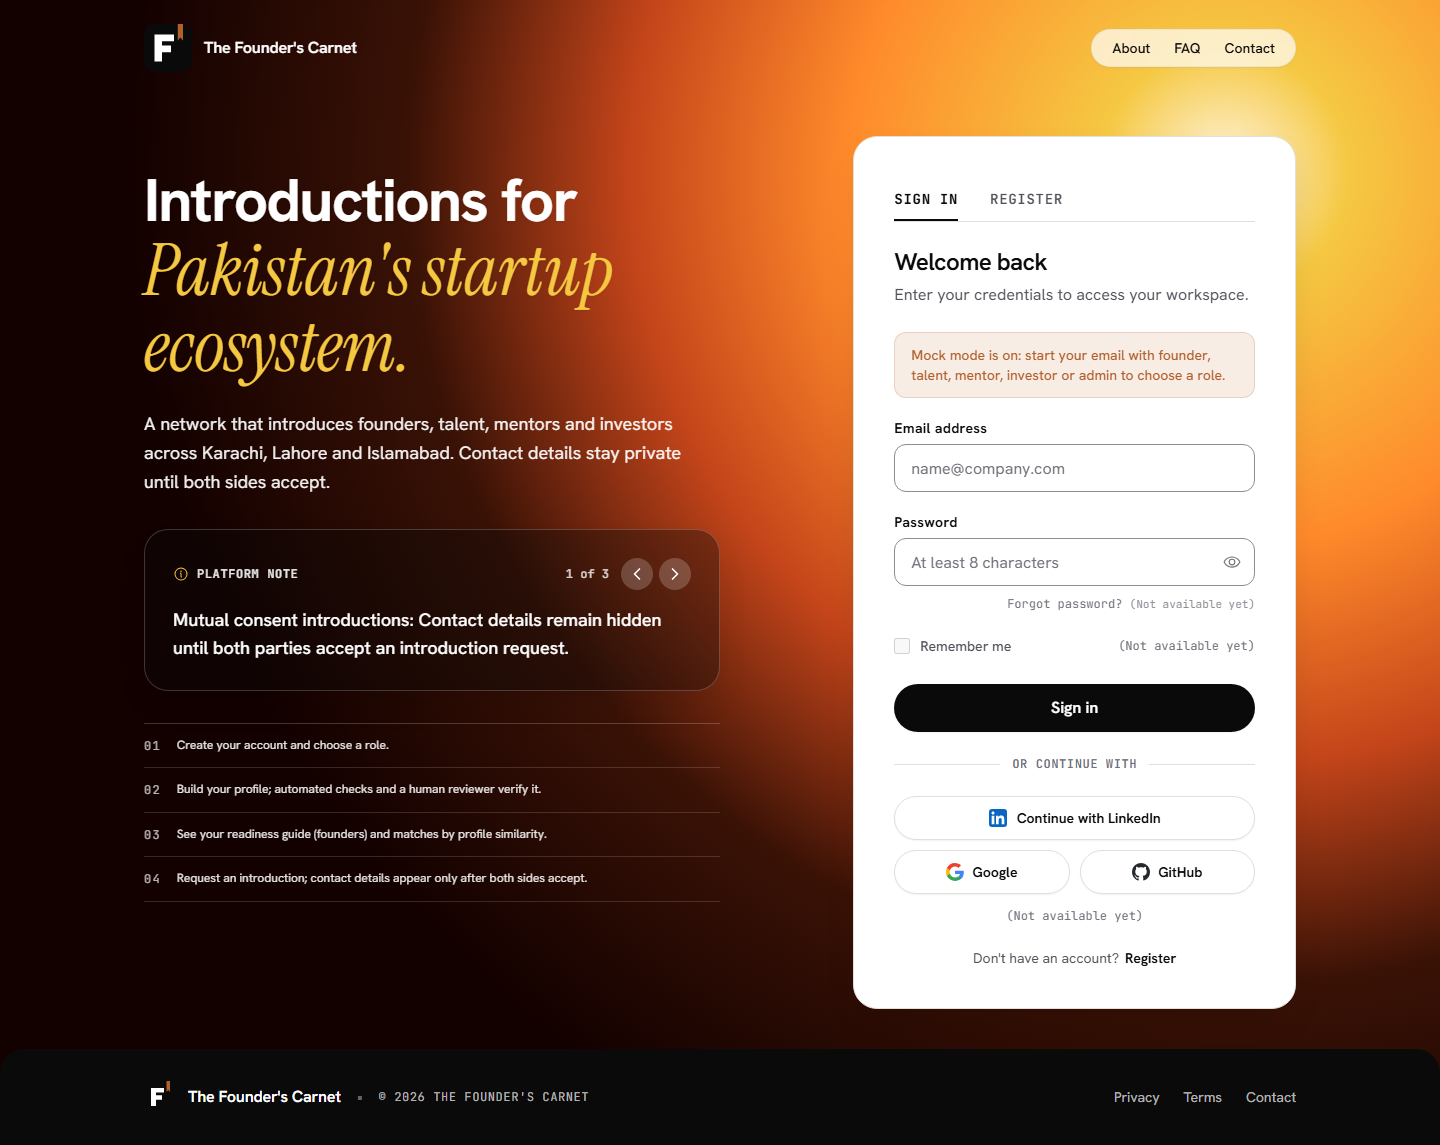
\includegraphics[width=\textwidth,height=0.50\textheight,keepaspectratio]{Figures/gui/auth.png}
\caption{Authentication Screen (FR-17, FR-22)}
\label{fig:gui-common}
\end{figure}

\begin{figure}[H]
\centering
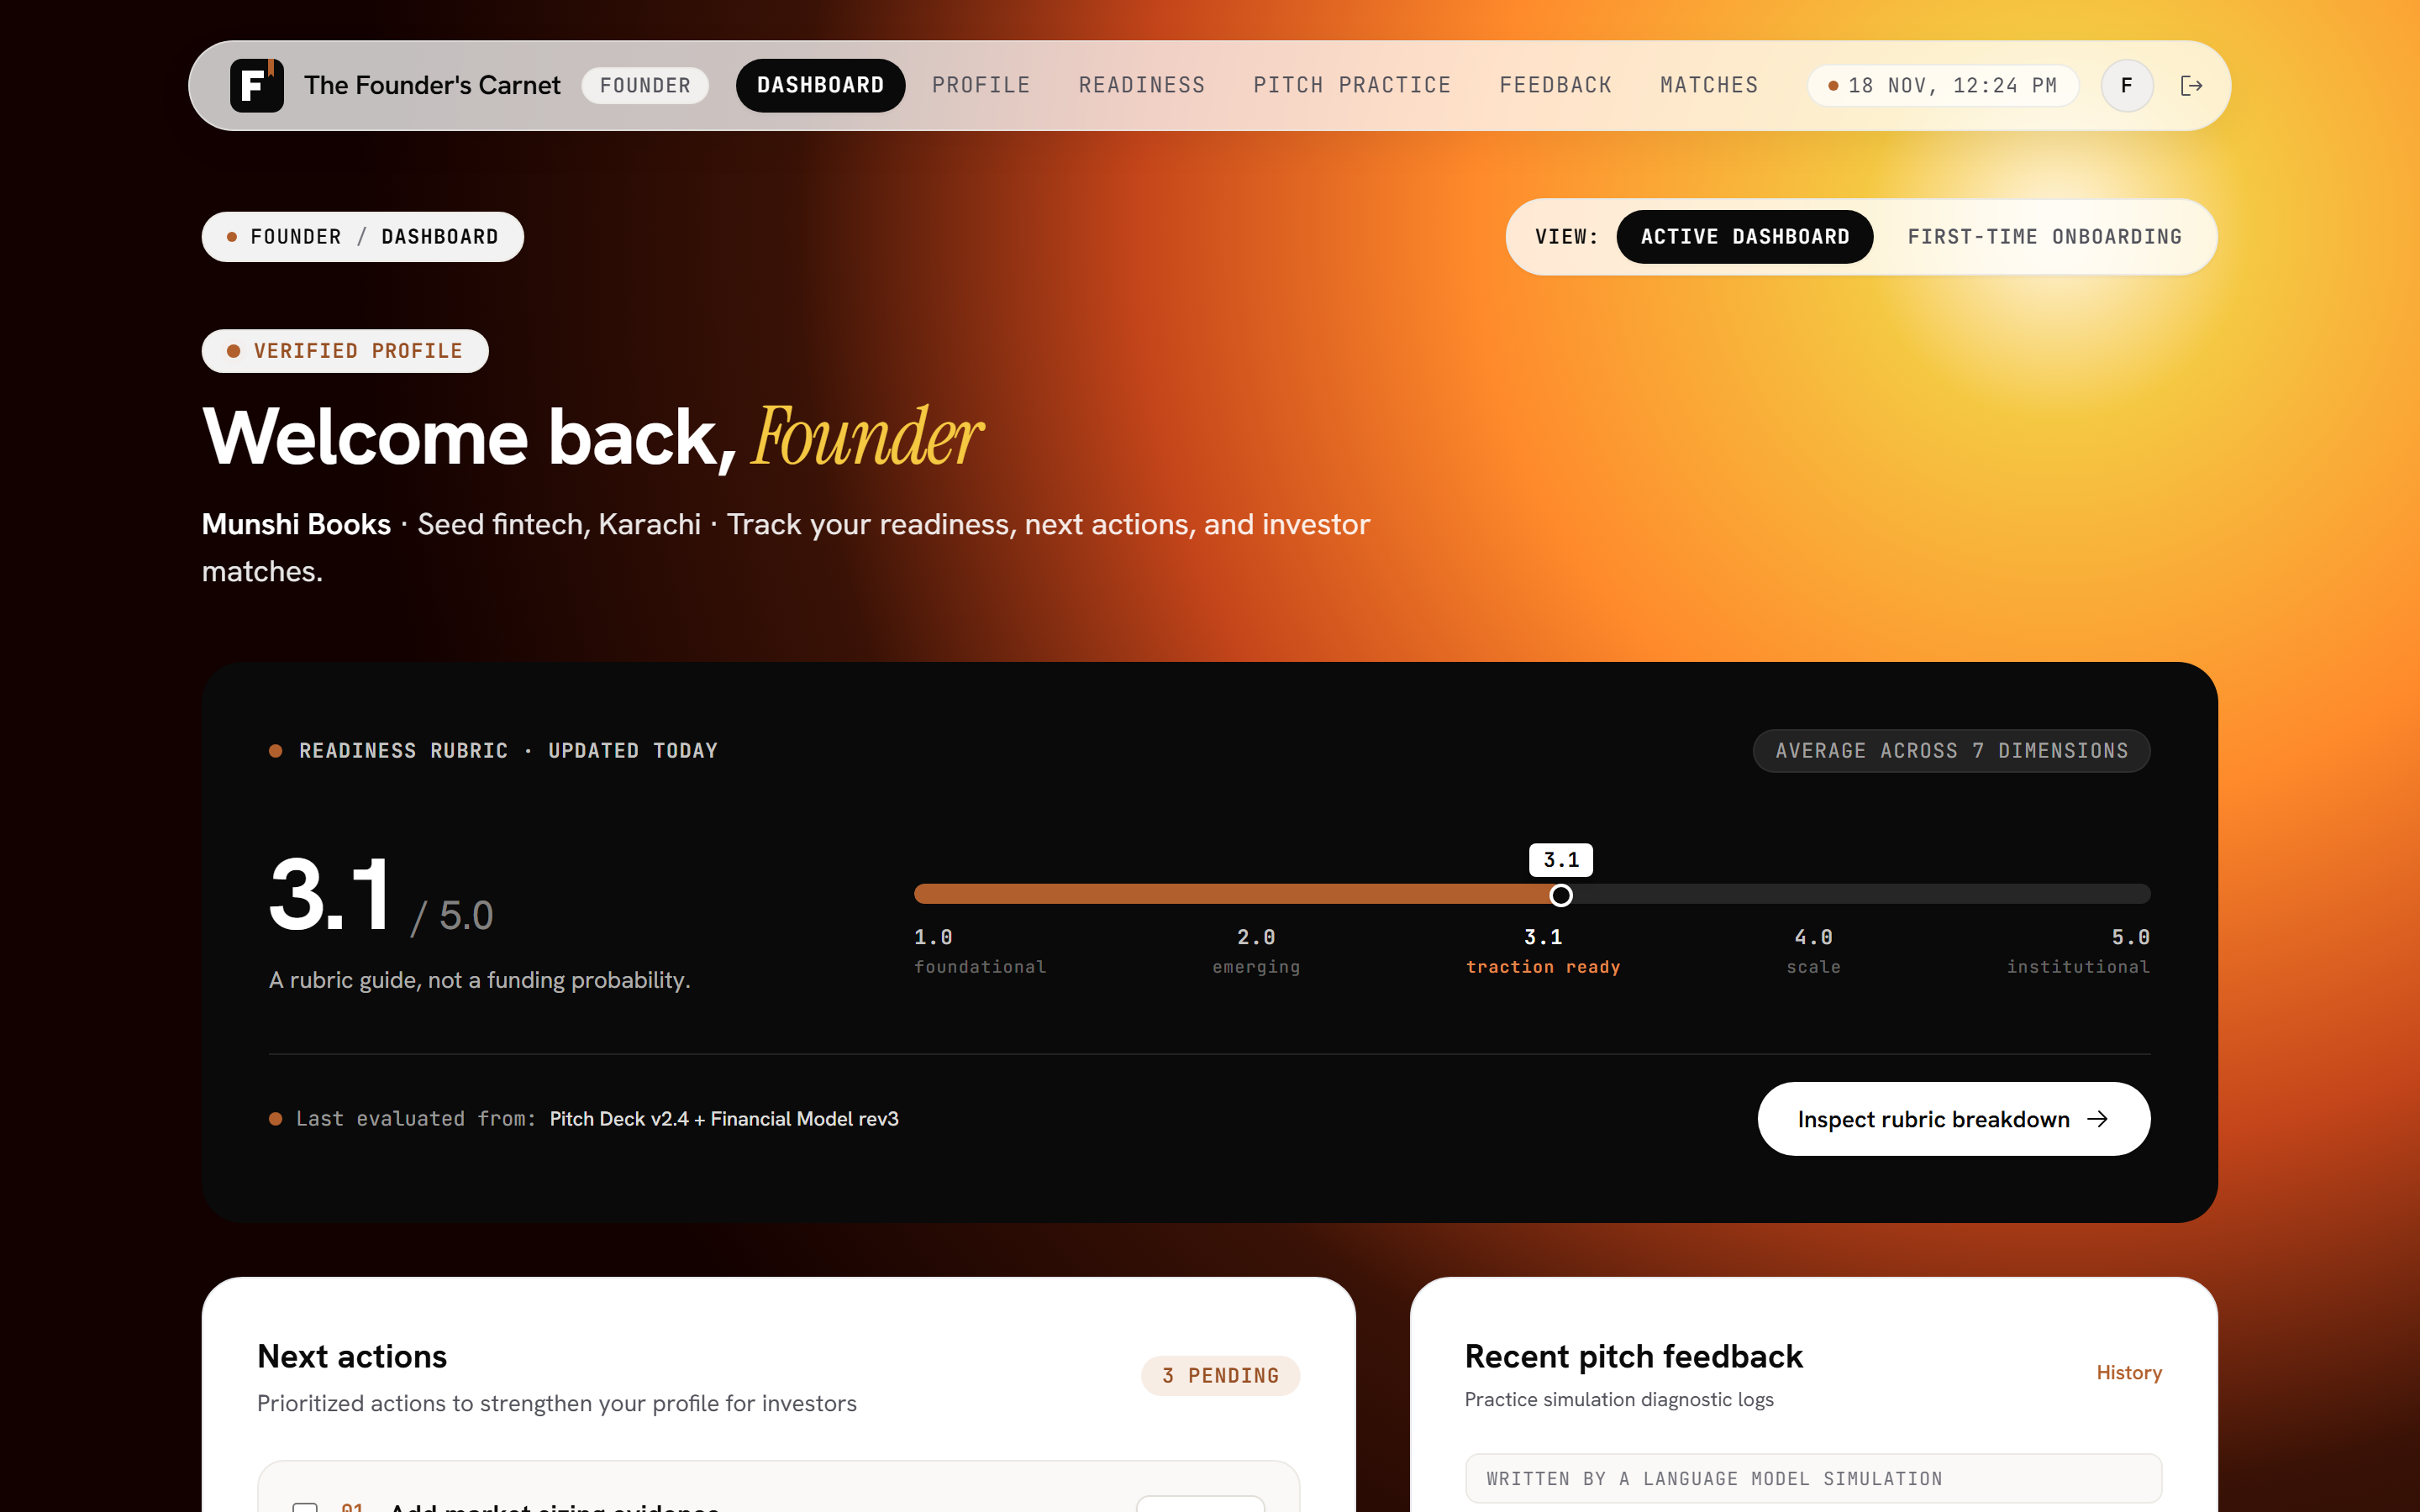
\includegraphics[width=\textwidth,height=0.40\textheight,keepaspectratio]{Figures/gui/founder_dashboard.png}
\caption{Founder Dashboard (FR-1, FR-2, FR-3, FR-7, FR-15)}
\label{fig:gui-founder}
\end{figure}

\begin{figure}[H]
\centering
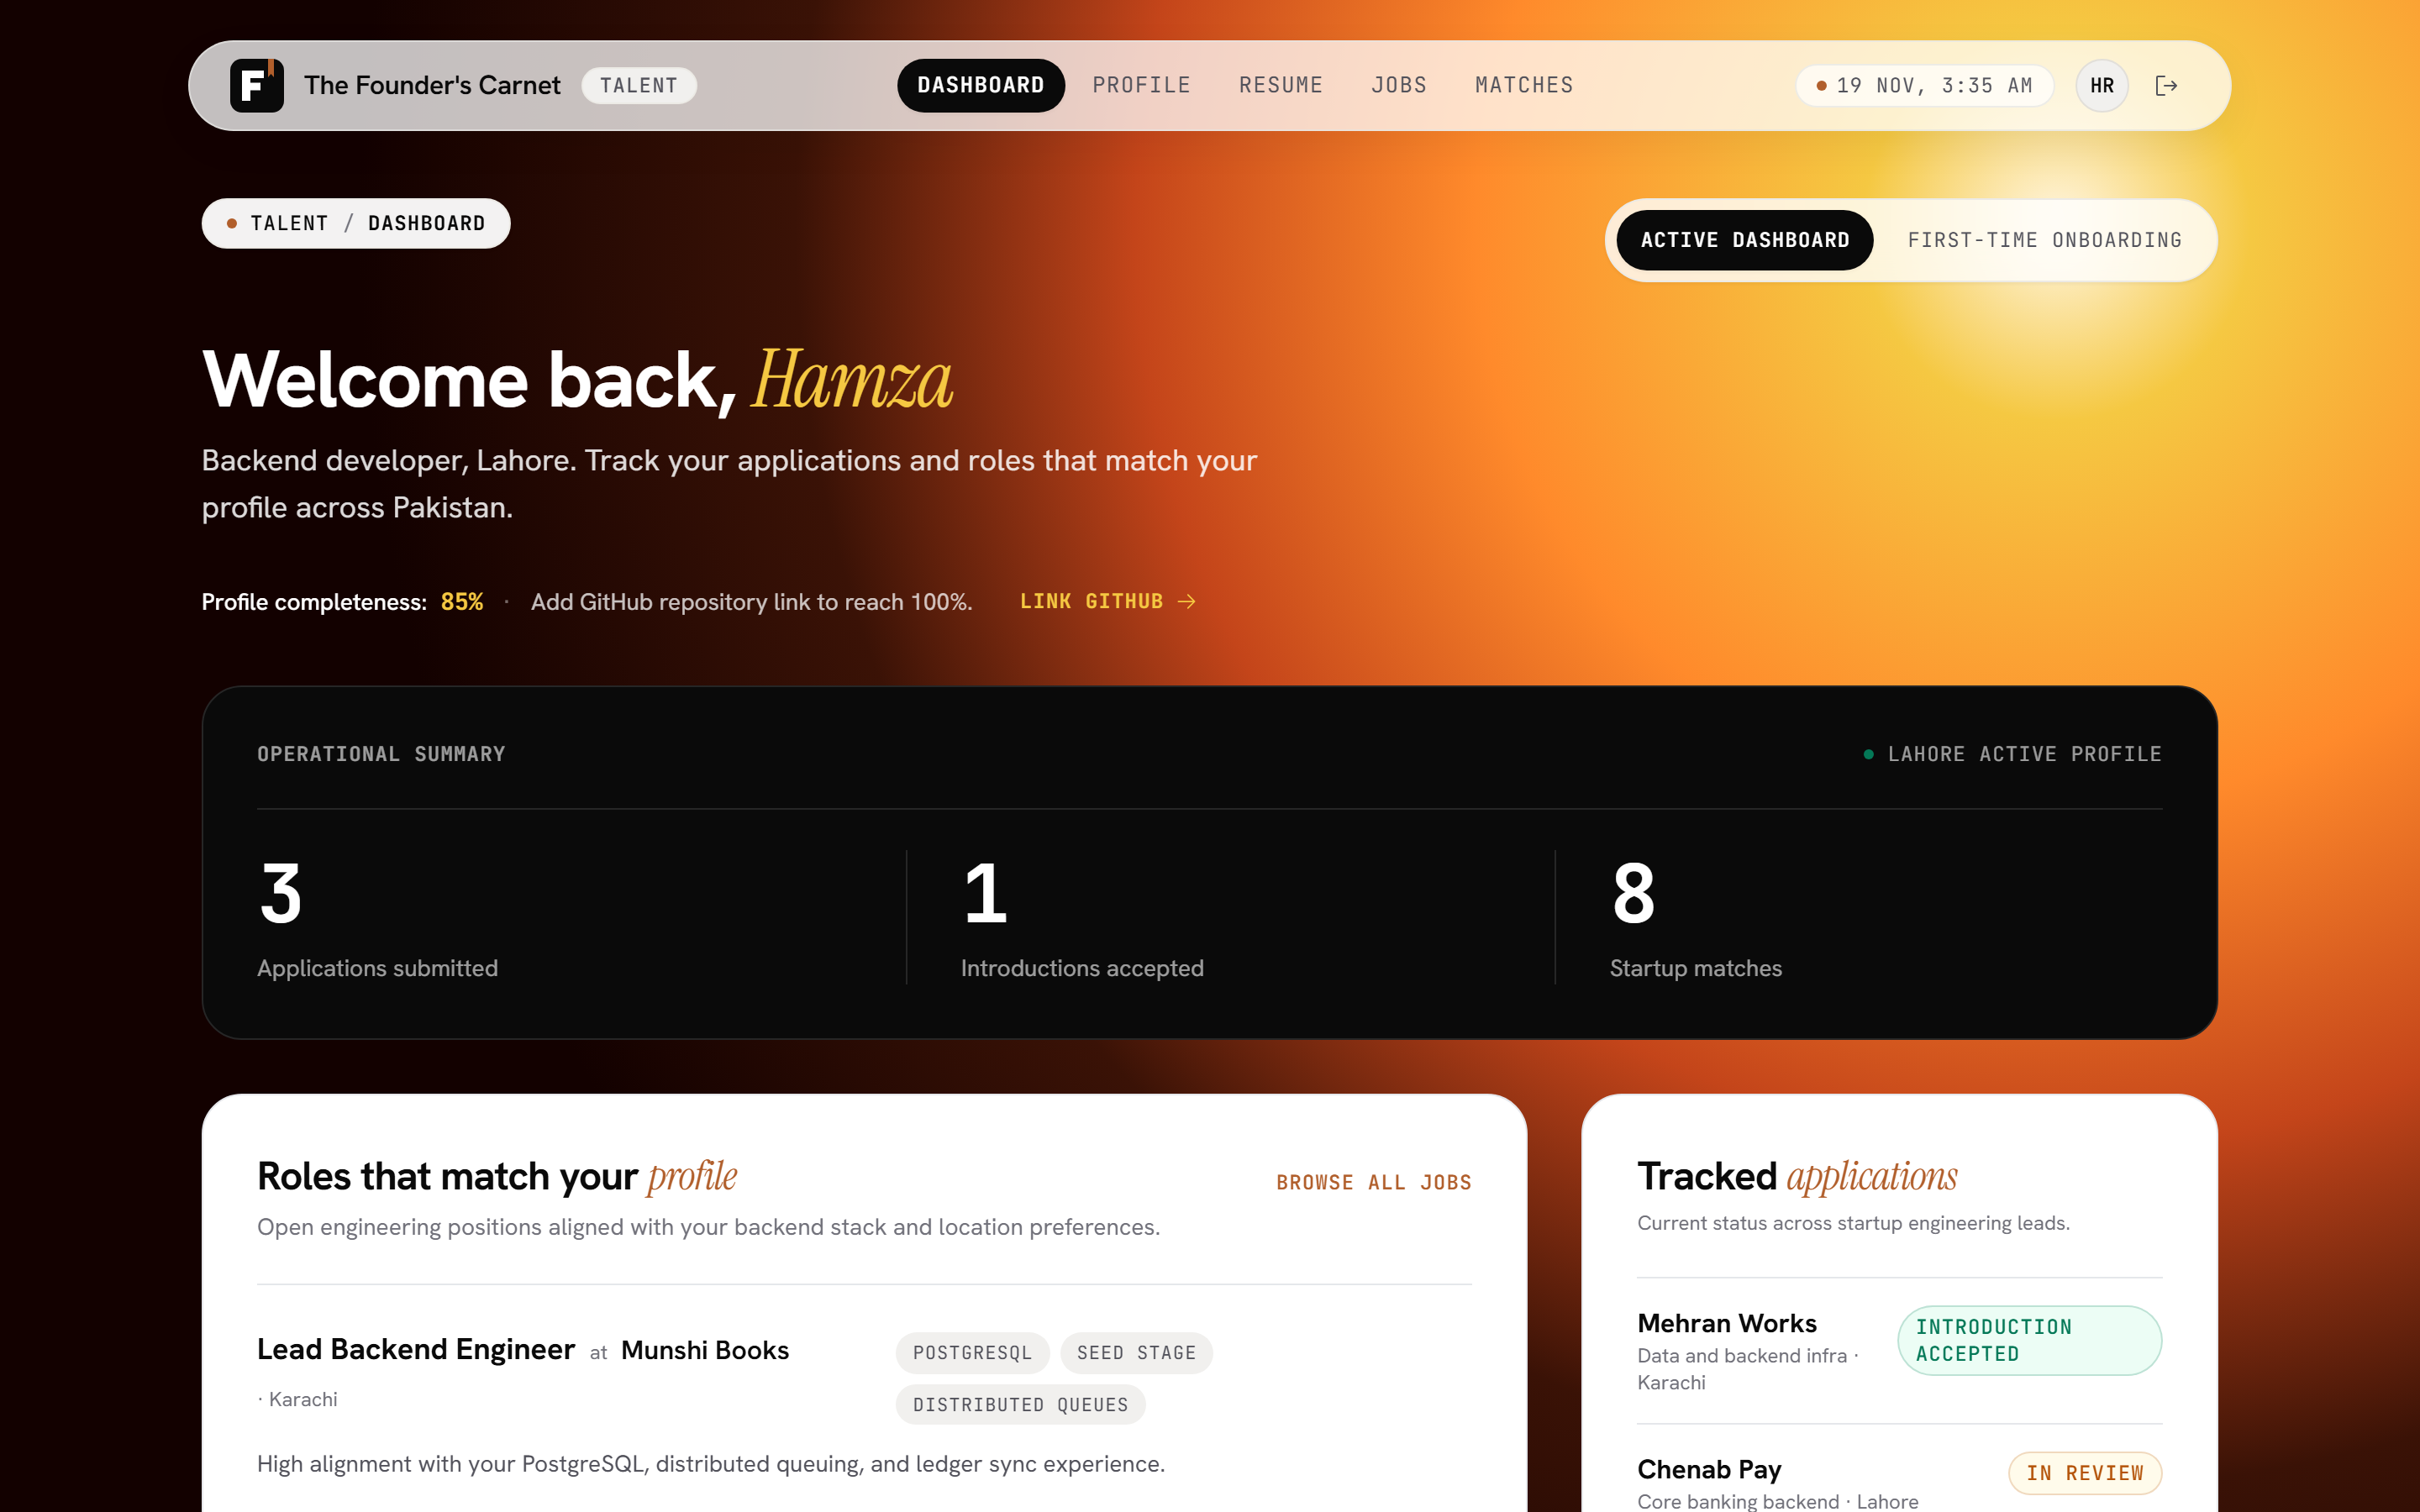
\includegraphics[width=\textwidth,height=0.40\textheight,keepaspectratio]{Figures/gui/talent_dashboard.png}
\caption{Talent Dashboard (FR-5, FR-6, FR-25)}
\label{fig:gui-talent}
\end{figure}

\begin{figure}[H]
\centering
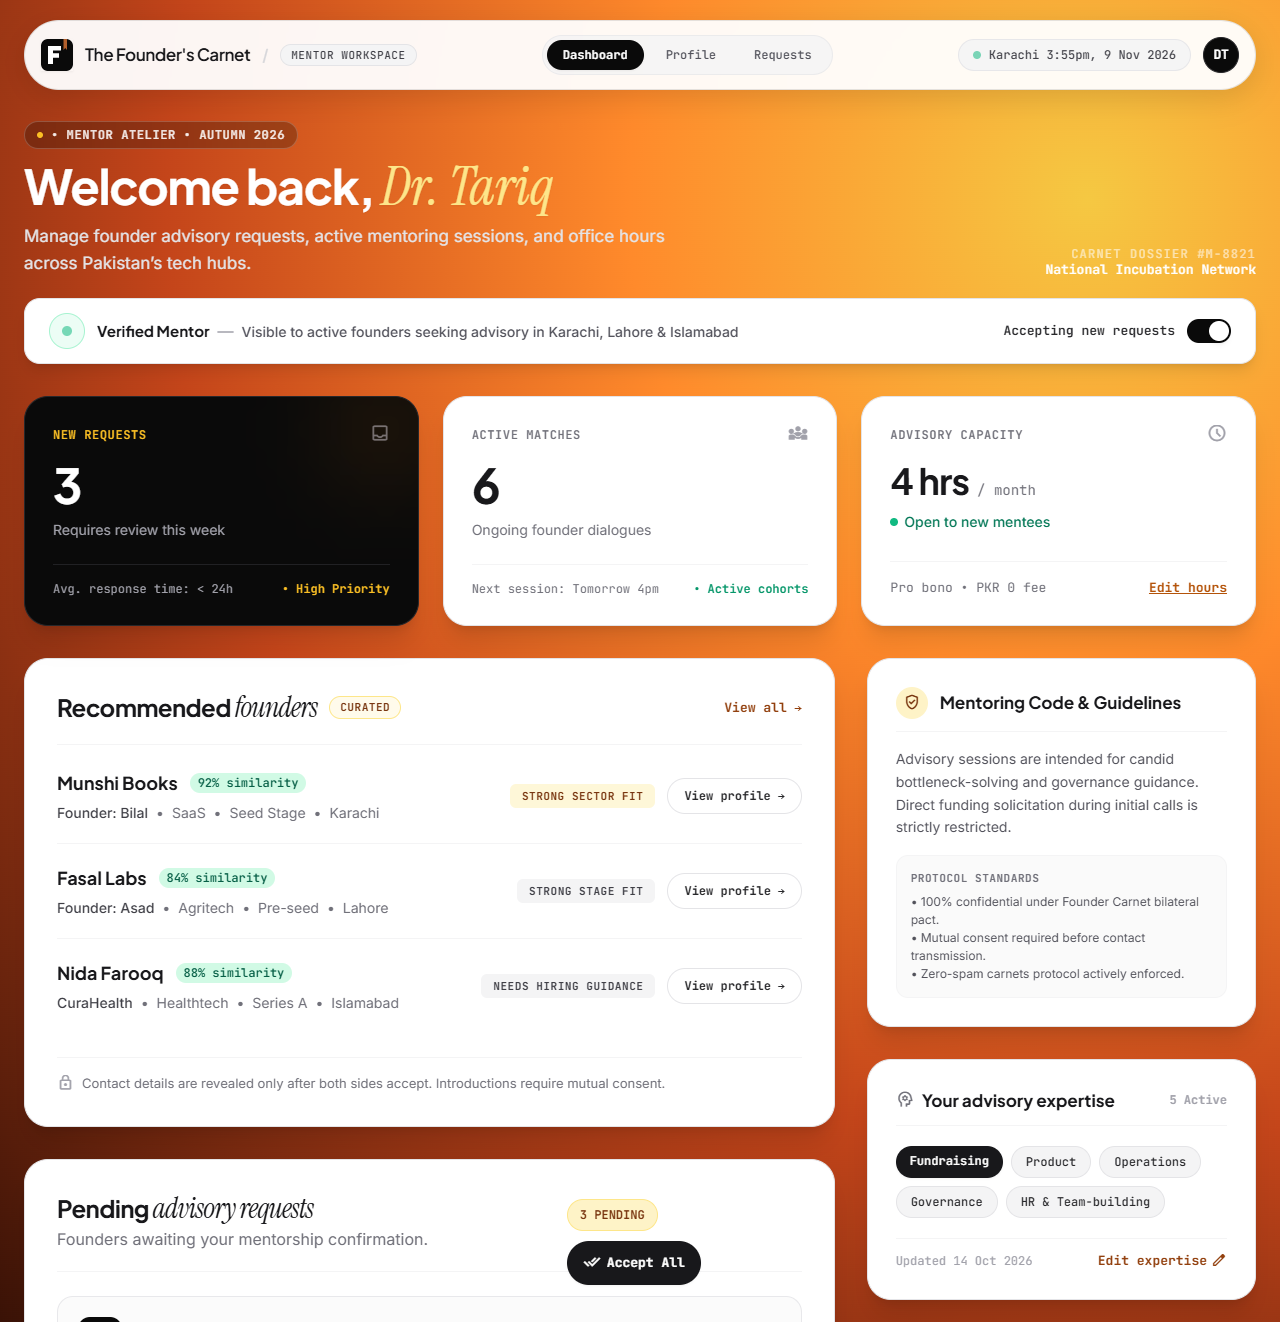
\includegraphics[width=\textwidth,height=0.40\textheight,keepaspectratio]{Figures/gui/mentor_dashboard.png}
\caption{Mentor Dashboard (FR-7, FR-29)}
\label{fig:gui-mentor}
\end{figure}

\begin{figure}[H]
\centering
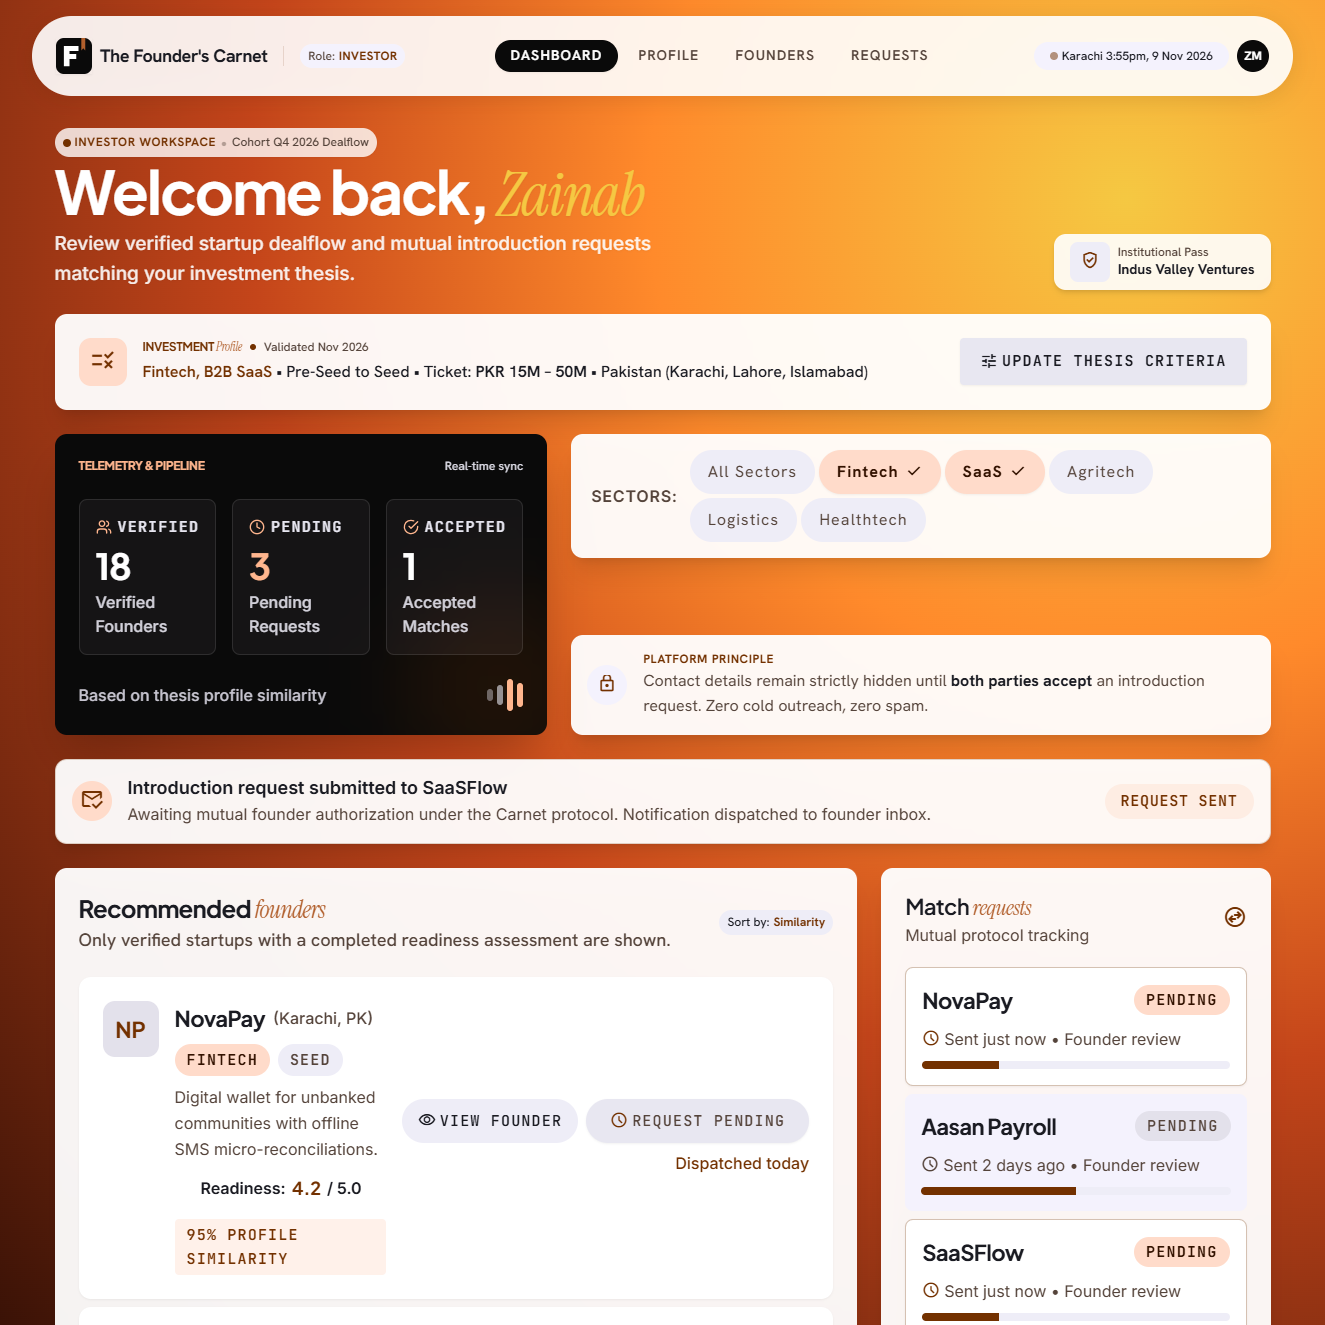
\includegraphics[width=\textwidth,height=0.40\textheight,keepaspectratio]{Figures/gui/investor_dashboard.png}
\caption{Investor Dashboard (FR-7, FR-10)}
\label{fig:gui-investor}
\end{figure}


\section{Database Design}\label{sec:db}
All its data is stored in one PostgreSQL database and stored in the vector database embeddings using the pgvector extension. The planned schema has 41 tables in five modules, which are accounts, profiles and consent (11 tables), verification, appeals and audit (6), founder services (10), matching, job board and applications (9), and the compliance corpus and query log (5). Some tables are already implemented while for FYP-2 features, the tables are created later. The ER diagrams represent the total design, and the data dictionary specifies the basic tables.


\subsection{Entity-Relationship (ER) Diagram}
The ER diagram is divided into one figure for every module to make it legible for viewing. Figures~\ref{fig:er-accounts} to~\ref{fig:er-compliance} show the tables of each module with their primary and foreign keys.

The accounts module has eleven tables as shown in figure~\ref{fig:er-accounts}. One \texttt{user\_account} row, and one profile for each user and each role. The expertise areas and thesis sectors are listed by mentors and investors in join tables, and there are tables for LinkedIn sign-in or GitHub sign-in that connect to an account. To store each notice that has been accepted and its version and time.

\begin{figure}[H]
    \centering
    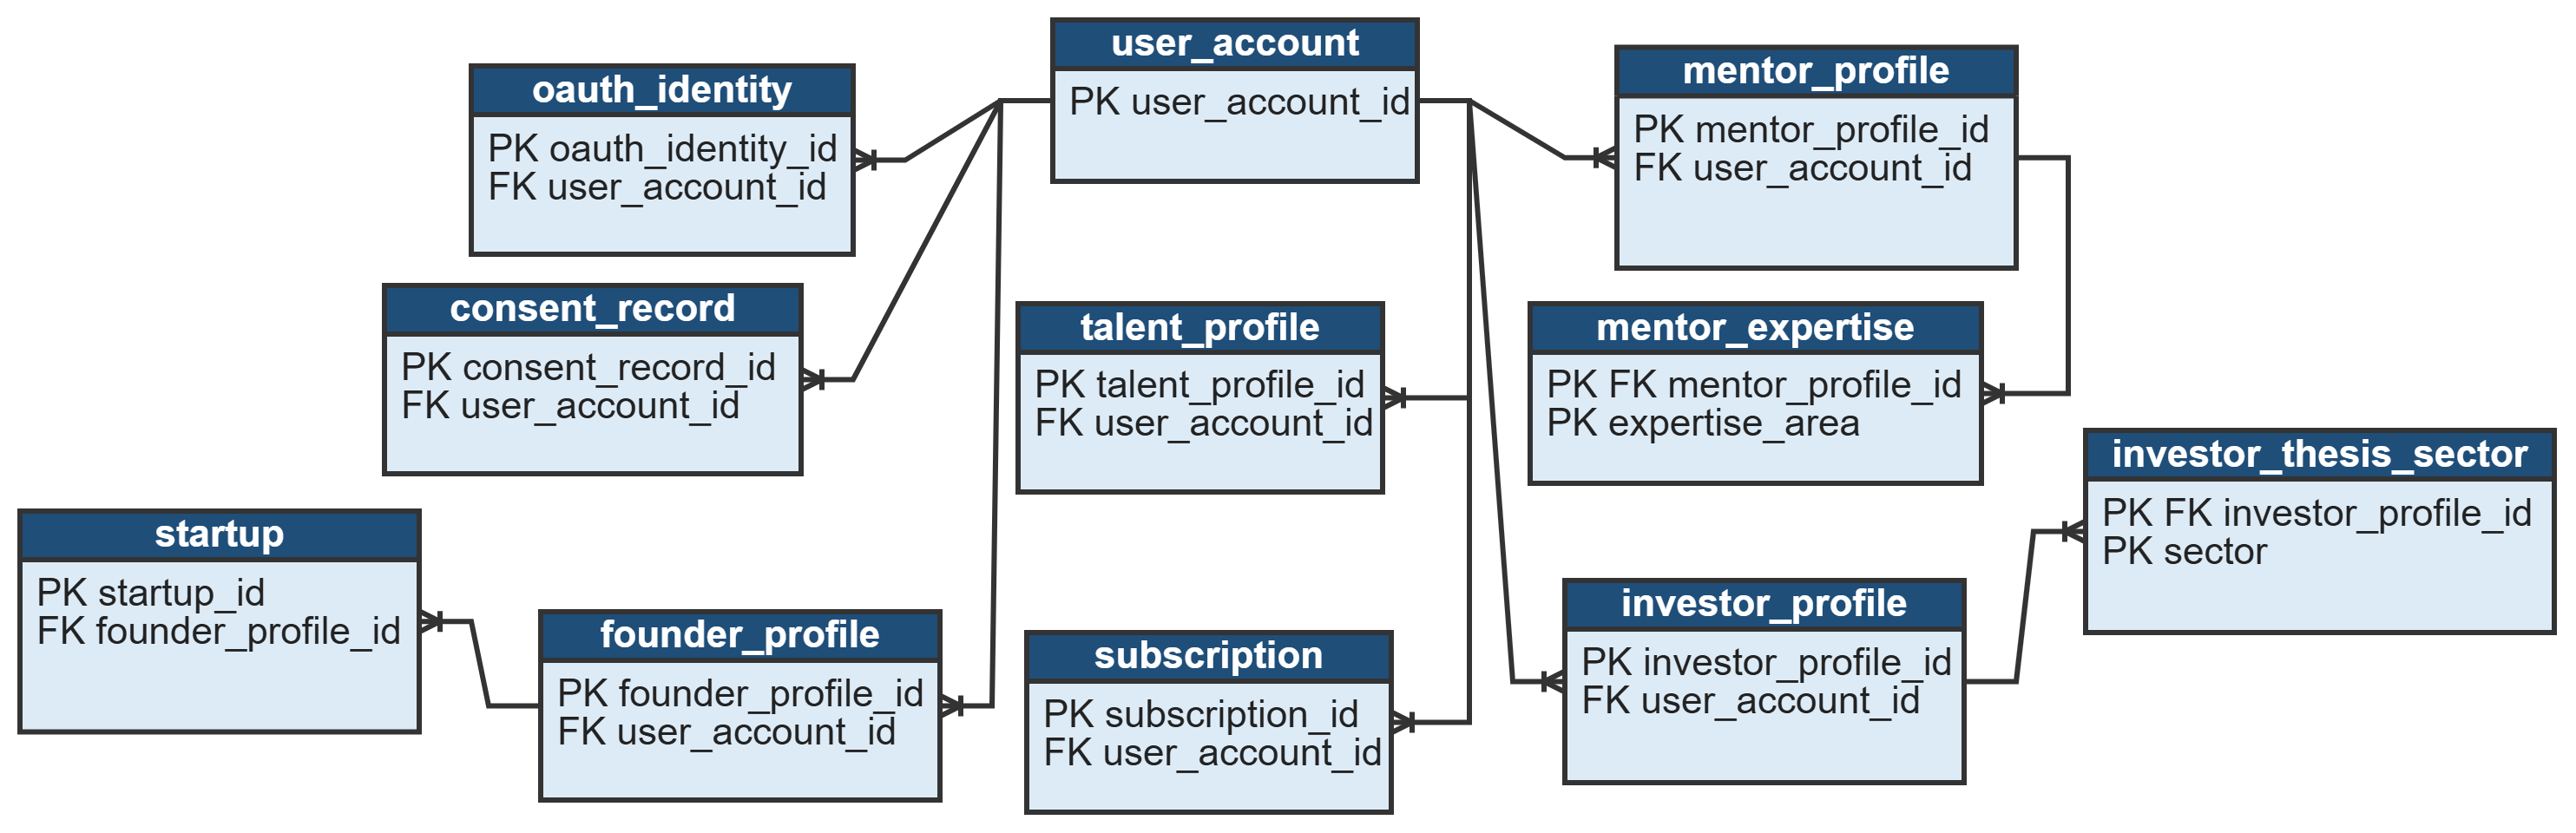
\includegraphics[width=\textwidth,height=0.5\textheight,keepaspectratio]{Figures/fig02_er_accounts}
    \caption{Accounts, Profiles and Consent Module}
    \label{fig:er-accounts}
\end{figure}

The founder services module has ten tables as shown in figure~\ref{fig:er-founder}. With each readiness assessment, pitch session and market research output, the prompt and model version are captured and recorded with each result, allowing each result to be traced back to the prompt or model version. There is one score row for each of the 7 dimensions and a transcript and feedback items for the pitch session.

\begin{figure}[H]
    \centering
    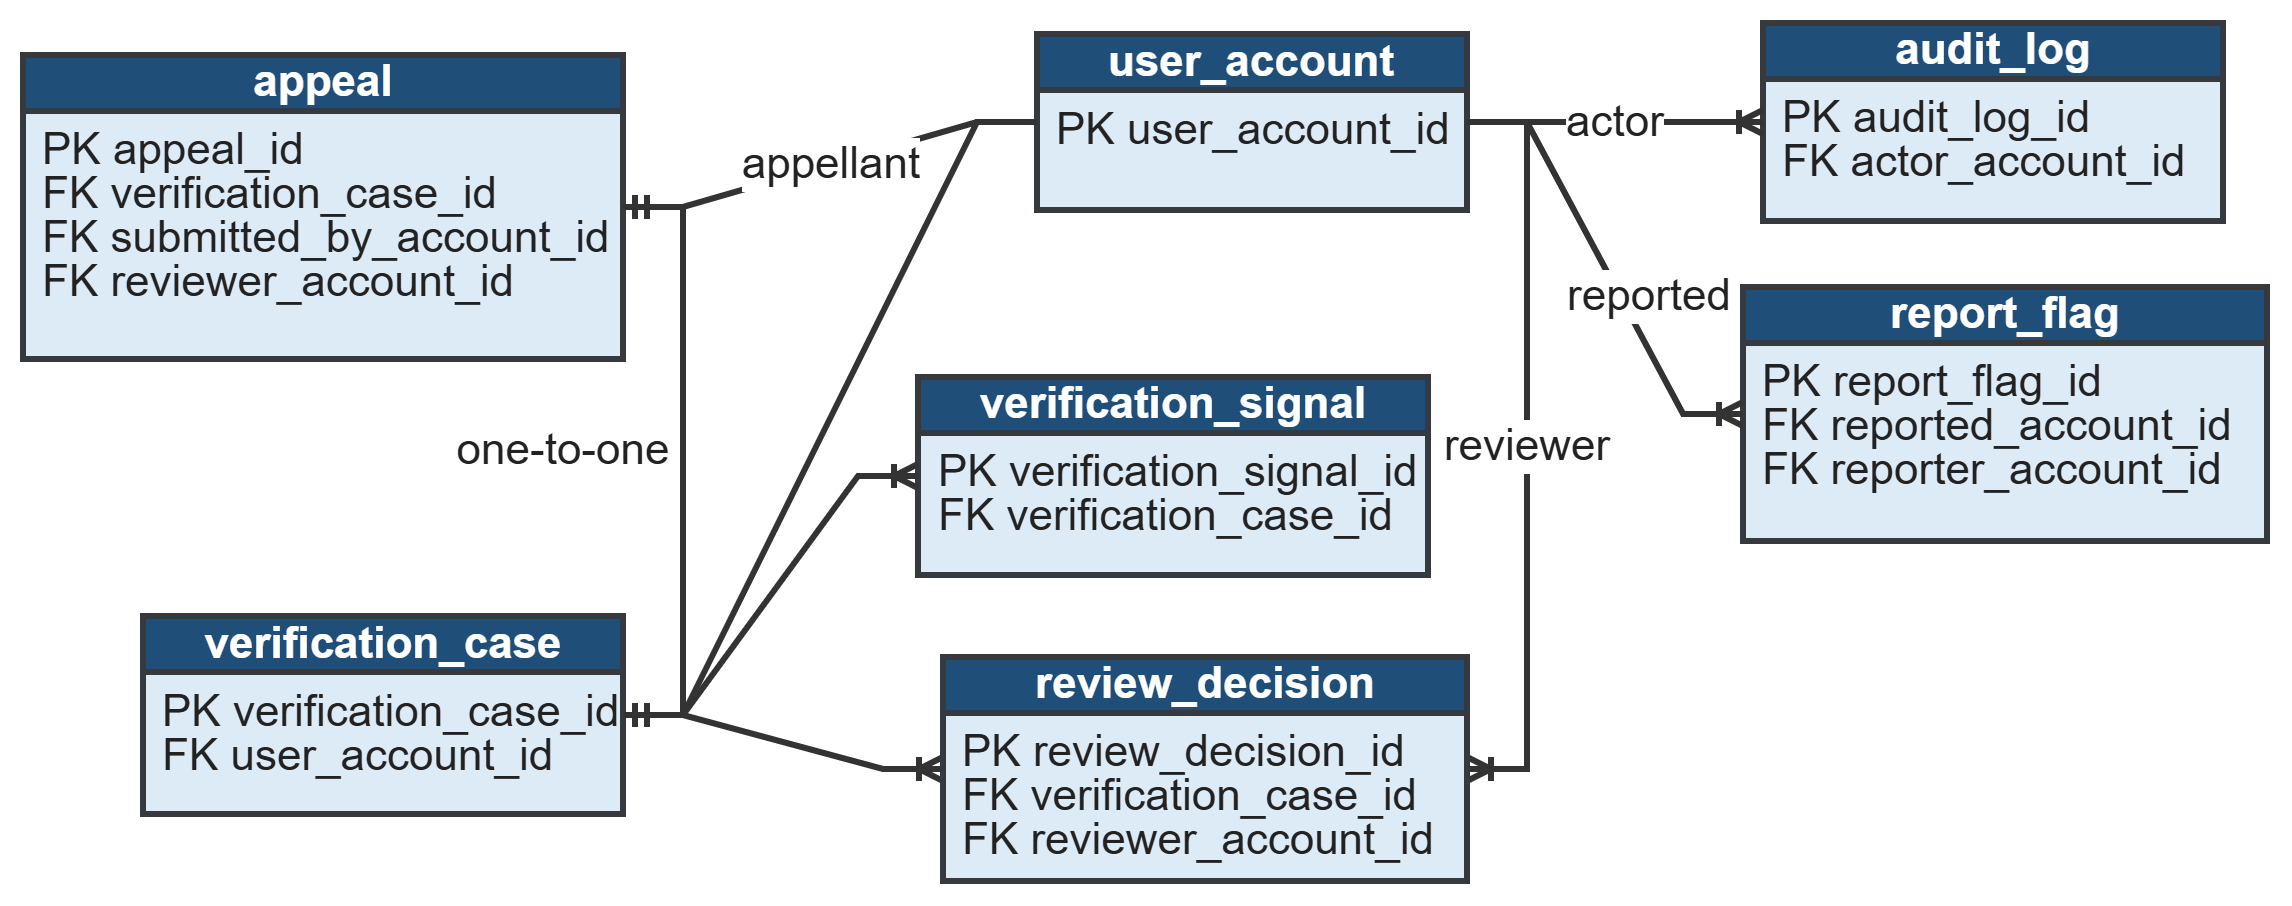
\includegraphics[width=\textwidth,height=0.5\textheight,keepaspectratio]{Figures/fig03_er_verification}
    \caption{Verification, Appeals and Audit Module}
    \label{fig:er-verification}
\end{figure}

The founder services module contains 10 tables as shown in figure~\ref{fig:er-founder}. Each readiness assessment, pitch session and market research output is captured with the prompt version and model version, which allows you to trace each output back to the prompt that produced it. The readiness assessment has 7 dimensions each with a score row, and a pitch session has a transcript and feedback items.

\begin{figure}[H]
    \centering
    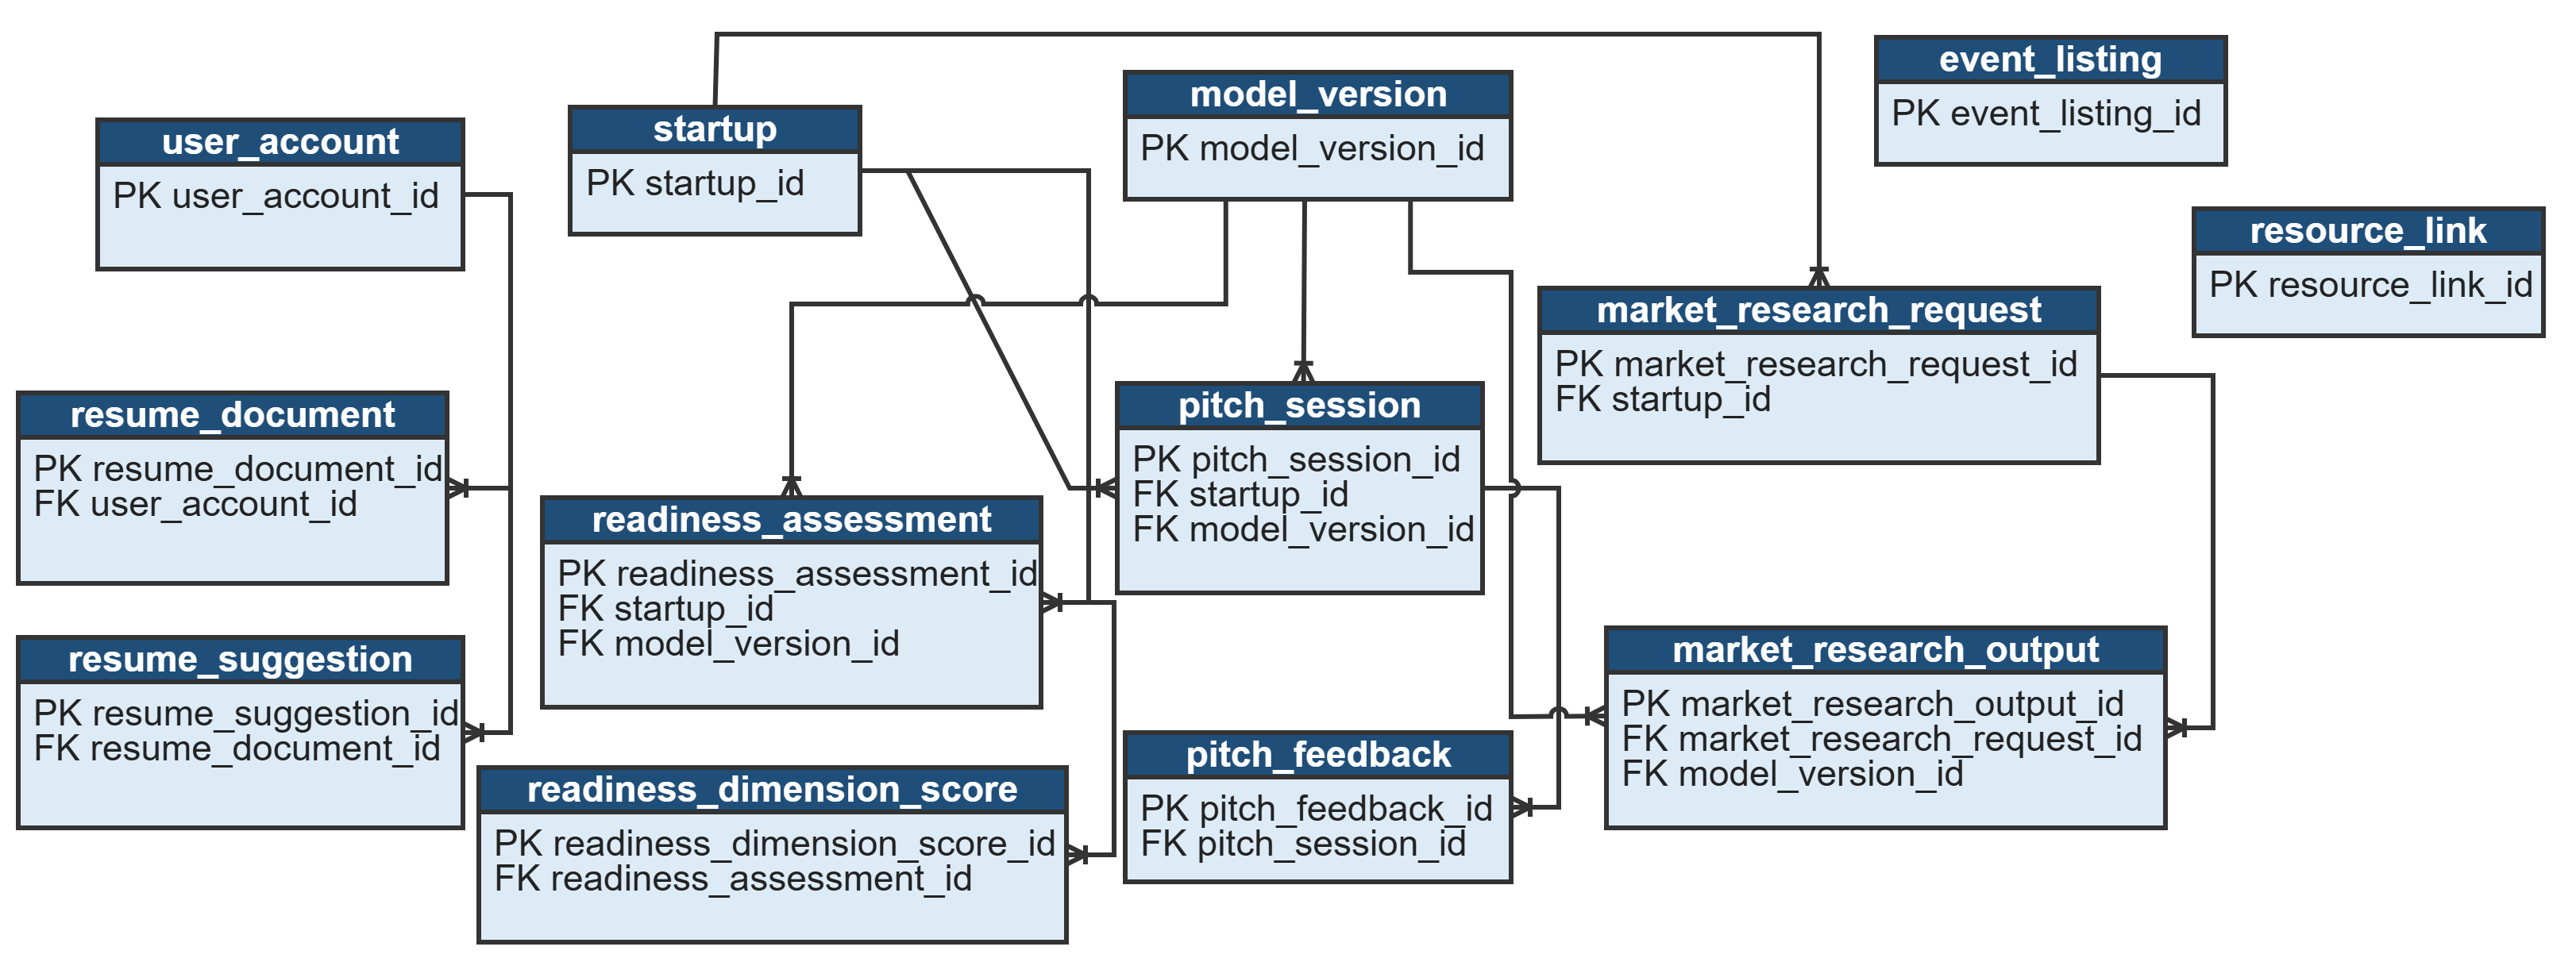
\includegraphics[width=\textwidth,height=0.5\textheight,keepaspectratio]{Figures/fig04_er_founder_services}
    \caption{Founder Services Module}
    \label{fig:er-founder}
\end{figure}

The matching and job board module, with nine tables, is shown in Figure~\ref{fig:er-matching}. A retrieval score, a reranking score and match factors, and the score remains empty until there is a reranker in FYP-2 Match request notifies if contact information is disclosed (which only occurs when both parties accept the exchange of information). There is one embeddings table that is used for profiles and job listings, and the placement fee table is created in FYP-2.

\begin{figure}[H]
    \centering
    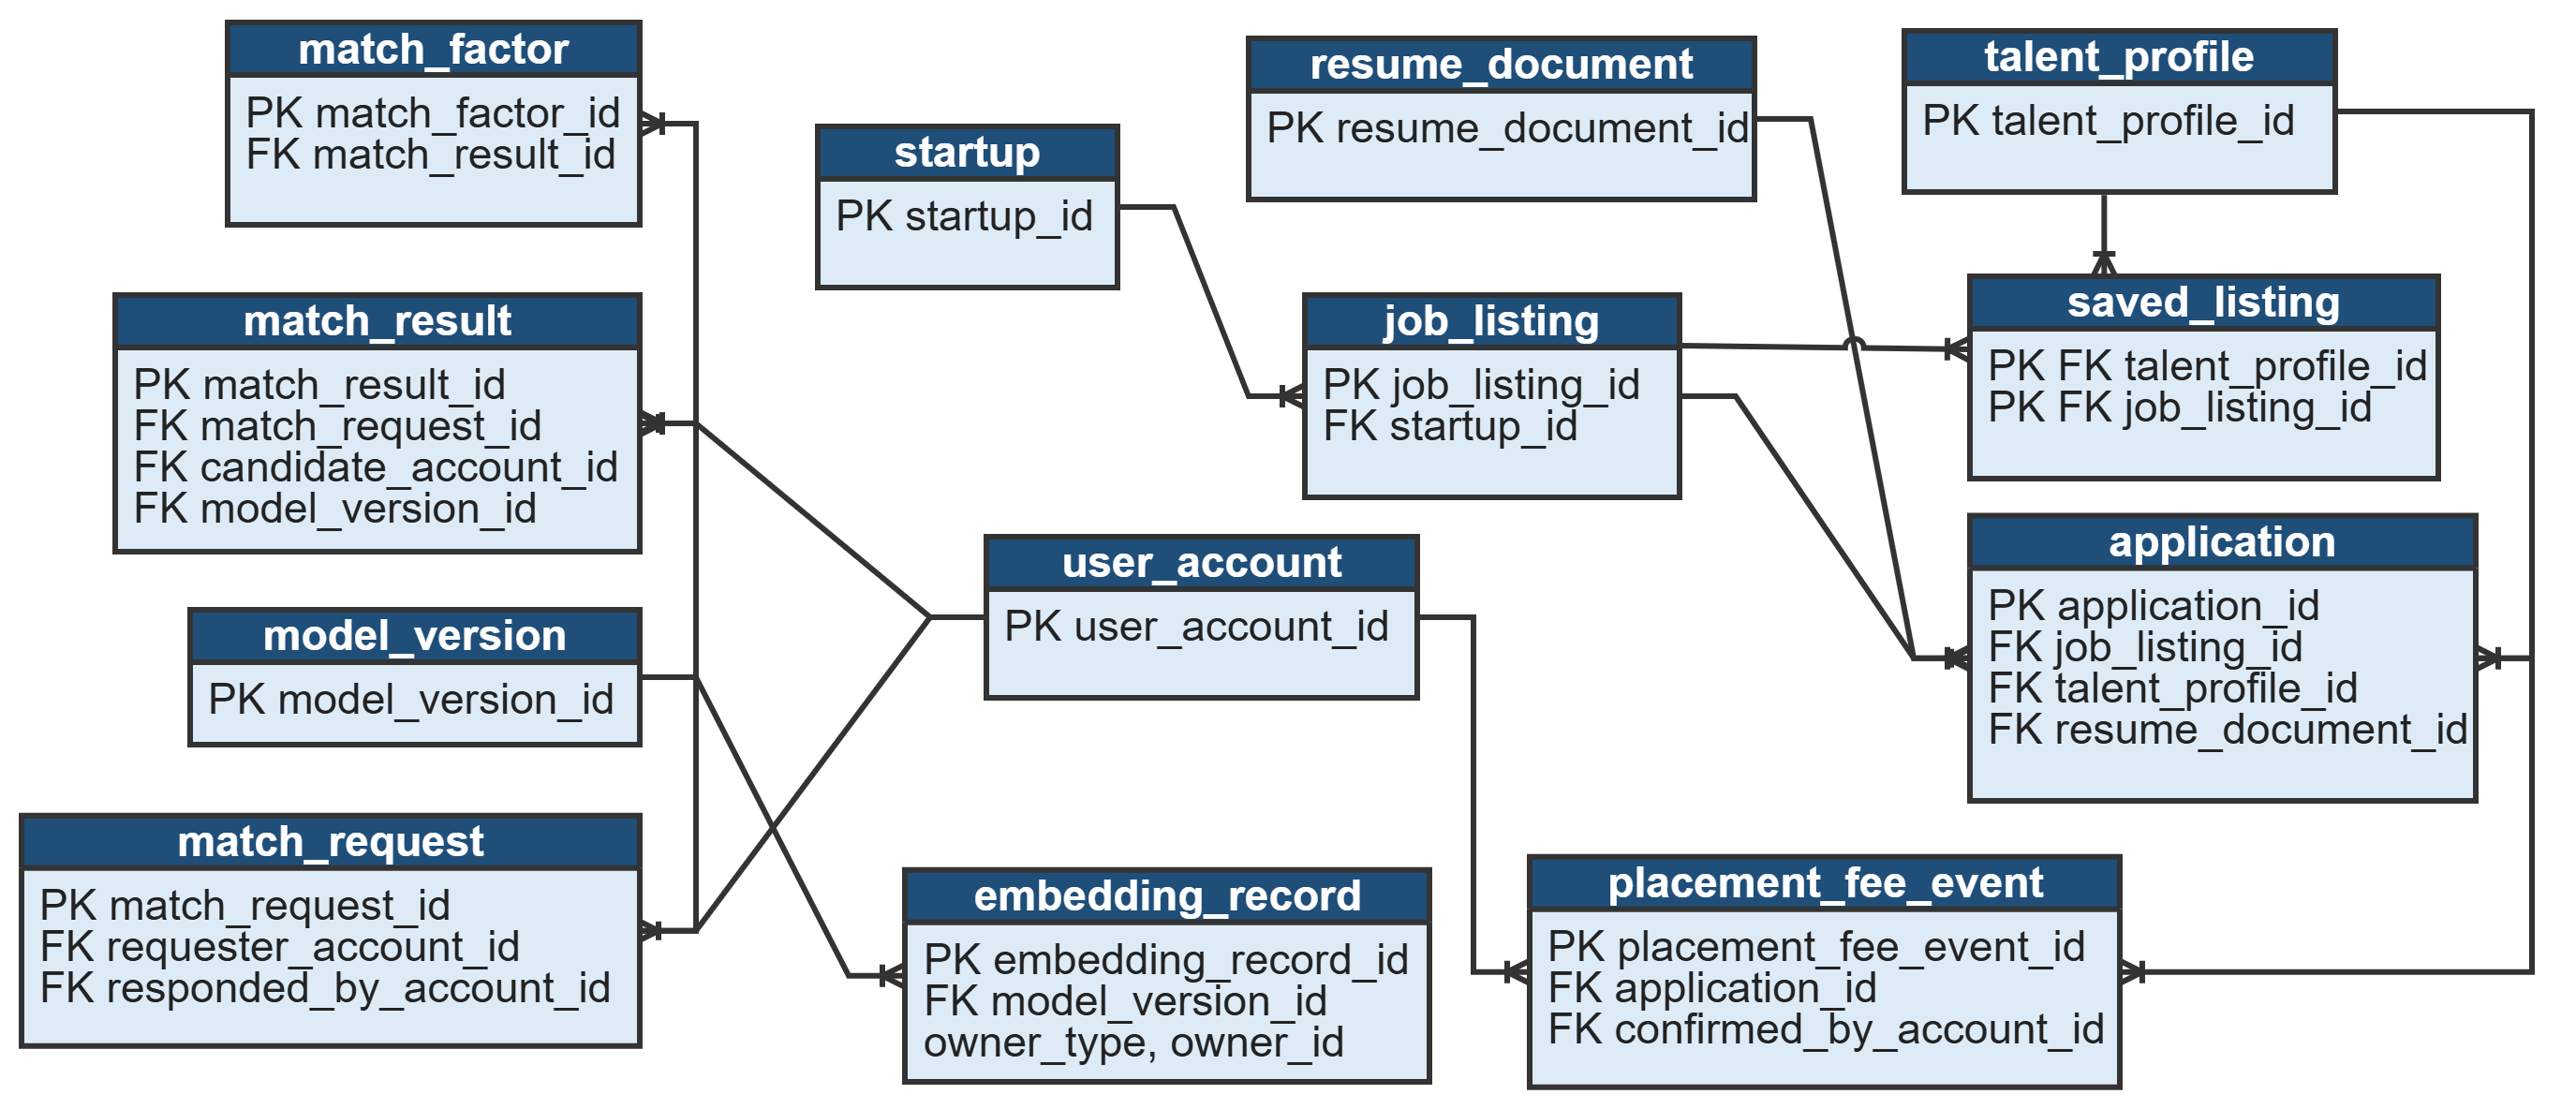
\includegraphics[width=\textwidth,height=0.5\textheight,keepaspectratio]{Figures/fig05_er_matching_jobs}
    \caption{Matching, Job Board and Applications Module}
    \label{fig:er-matching}
\end{figure}

The compliance module in figure~\ref{fig:er-compliance} contains five tables. Each source document is maintained and the effective and consolidation/retrieval dates and a SHA-256 hash of the document is recorded. Documents are divided into parts that preserves the section and page references. Each question is saved along with an answer to it and the outcome of whether it was answered, refused, or failed.

\begin{figure}[H]
    \centering
    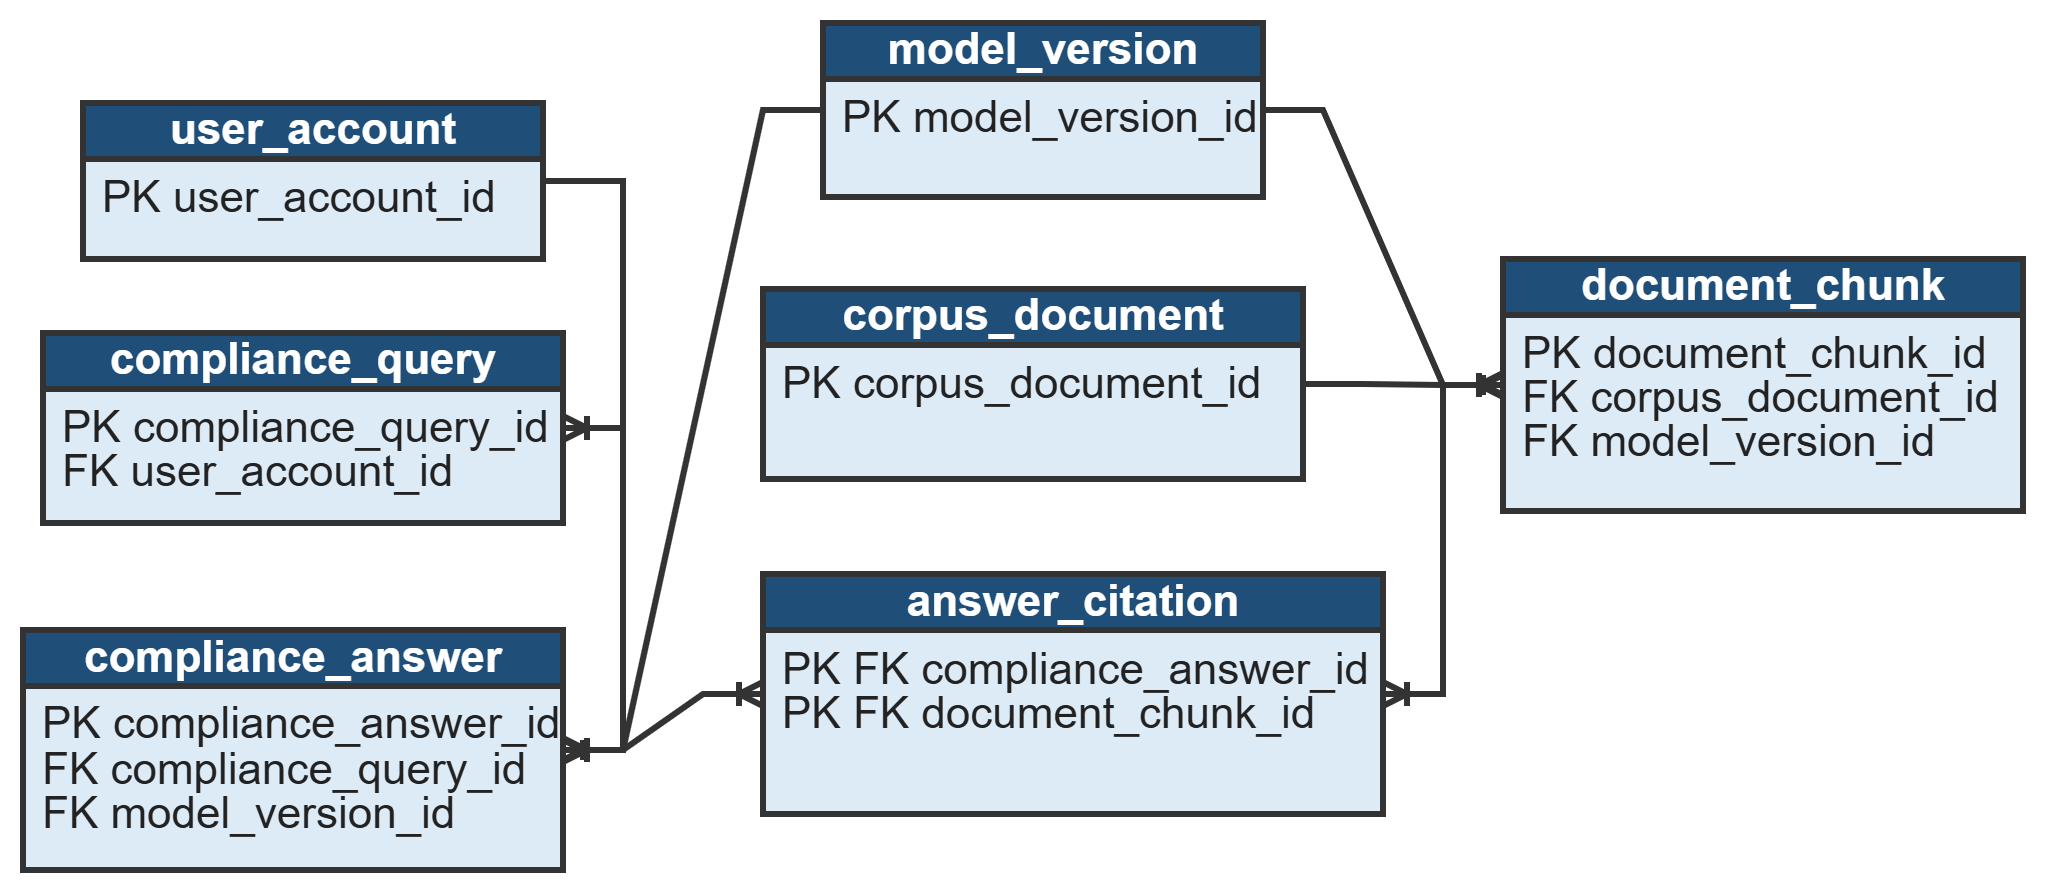
\includegraphics[width=\textwidth,height=0.5\textheight,keepaspectratio]{Figures/fig06_er_compliance}
    \caption{Compliance Corpus and Query Log Module}
    \label{fig:er-compliance}
\end{figure}

\subsection{Data Dictionary}
This data dictionary lists the core tables which features depend on in the planned database, that contains 41 tables and 264 attributes. Each table gets a name in its caption and its key attributes are listed with their PostgreSQL type, whether they can be null and what other table they are related to. The primary and foreign keys are indicated by PK and FK respectively. The status and type fields are text constrained and their allowed values are in the description field.

\begin{table}[!ht]
\centering
\caption{User Account table}
\label{tab:dd-user-account}
\begin{tabular}{|p{3.2cm}|p{2.5cm}|p{1.4cm}|p{2.9cm}|p{4.0cm}|}
\ddhead
user\_account\_id & integer (PK) & No &  & Unique identifier of the account \\ \hline
email & varchar(255) & No &  & Unique login email \\ \hline
full\_name & varchar(255) & No &  & Name of the user \\ \hline
password\_hash & varchar(255) & No &  & Salted password hash \\ \hline
role & varchar(50) & No &  & founder, talent, mentor, investor or admin \\ \hline
is\_active & boolean & No &  & False when the account is disabled \\ \hline
\end{tabular}
\end{table}

\begin{table}[!ht]
\centering
\caption{Readiness Assessment table}
\label{tab:dd-readiness-assessment}
\begin{tabular}{|p{3.2cm}|p{2.5cm}|p{1.4cm}|p{2.9cm}|p{4.0cm}|}
\ddhead
readiness\_assessment\_id & integer (PK) & No &  & Unique identifier of the assessment \\ \hline
startup\_id & integer (FK) & No & startup, One-to-Many & Startup that was assessed \\ \hline
model\_version\_id & integer (FK) & No & model\_version, One-to-Many & Model and prompt used for the scoring \\ \hline
overall\_score & numeric(5,2) & No &  & Combined score over the seven dimensions \\ \hline
\end{tabular}
\end{table}

\begin{table}[!ht]
\centering
\caption{Document Chunk table}
\label{tab:dd-document-chunk}
\begin{tabular}{|p{3.2cm}|p{2.5cm}|p{1.4cm}|p{2.9cm}|p{4.0cm}|}
\ddhead
document\_chunk\_id & integer (PK) & No &  & Unique identifier of the passage \\ \hline
corpus\_document\_id & integer (FK) & No & corpus\_document, One-to-Many & Document that the passage comes from \\ \hline
model\_version\_id & integer (FK) & No & model\_version, One-to-Many & Embedding model used for the passage \\ \hline
page\_number & integer & No &  & Page of the passage \\ \hline
chunk\_text & text & No &  & Text of the passage \\ \hline
embedding & vector & Yes &  & Embedding used for retrieval \\ \hline
\end{tabular}
\end{table}

\begin{table}[!ht]
\centering
\caption{Compliance Answer table}
\label{tab:dd-compliance-answer}
\begin{tabular}{|p{3.2cm}|p{2.5cm}|p{1.4cm}|p{2.9cm}|p{4.0cm}|}
\ddhead
compliance\_answer\_id & integer (PK) & No &  & Unique identifier of ans \\ \hline
compliance\_query\_id & integer (FK) & No & compliance\_query, One-to-Many & Question that was answered \\ \hline
model\_version\_id & integer (FK) & No & model\_version, One-to-Many & Model and prompt used for the answer \\ \hline
answer\_text & text & Yes &  & Text of the answer \\ \hline
outcome & varchar(20) & No &  & answer, refuse, fail \\ \hline
refusal\_reason & varchar(100) & Yes &  & Reason for refusing ans \\ \hline
latency\_ms & integer & No &  & Response time in ms \\ \hline
\end{tabular}
\end{table}

\begin{table}[!ht]
\centering
\caption{Startup Table}
\label{tab:dd-startup}
\begin{tabular}{|p{3.2cm}|p{2.5cm}|p{1.4cm}|p{2.9cm}|p{4.0cm}|}
\ddhead
startup\_id & integer (PK) & No &  & Unique identifier of the startup \\ \hline
founder\_profile\_id & integer (FK) & No & founder\_profile, One-to-Many & Founder who owns the startup \\ \hline
name & varchar(255) & No &  & Startup name \\ \hline
description & text & No &  & What the startup does \\ \hline
sector & varchar(100) & No &  & Industry sector \\ \hline
stage & varchar(30) & No &  & idea, mvp, growth or scaling \\ \hline
location & varchar(255) & No &  & City of operation \\ \hline
business\_model & varchar(255) & No &  & How the startup earns revenue \\ \hline
customer\_count & integer & No &  & Number of customers, zero or more \\ \hline
monthly\_revenue & numeric(14,2) & Yes &  & Monthly revenue, zero or more \\ \hline
required\_skills & json & No &  & Skills the startup needs \\ \hline
funding\_need\_min & numeric(14,2) & Yes &  & Lower end of the funding need \\ \hline
funding\_need\_max & numeric(14,2) & Yes &  & Upper end, not below the lower end \\ \hline
is\_verified & boolean & No &  & True once the profile is verified \\ \hline
\end{tabular}
\end{table}

\begin{table}[!ht]
\centering
\caption{Mentor Profile table}
\label{tab:dd-mentor-profile}
\begin{tabular}{|p{3.2cm}|p{2.5cm}|p{1.4cm}|p{2.9cm}|p{4.0cm}|}
\ddhead
mentor\_profile\_id & integer (PK) & No &  & Unique identifier of the mentor profile \\ \hline
user\_account\_id & integer (FK) & No & user\_account, One-to-One & Account that owns the profile \\ \hline
summary & text & No &  & Short description of the mentor and the experience offered \\ \hline
stage\_focus & json & No &  & Startup stages the mentor supports \\ \hline
location & varchar(255) & No &  & City of the mentor \\ \hline
availability & varchar(30) & No &  & Current availability for new mentees \\ \hline
is\_open & boolean & No &  & False when the mentor has closed the profile to new matches (FR-29) \\ \hline
consent\_version & varchar(50) & No &  & Version of the consent notice that was accepted \\ \hline
consented\_at & timestamp & No &  & Time the consent was given \\ \hline
\end{tabular}
\end{table}

\begin{table}[!ht]
\centering
\caption{Match Result table}
\label{tab:dd-match-result}
\begin{tabular}{|p{3.2cm}|p{2.5cm}|p{1.4cm}|p{2.9cm}|p{4.0cm}|}
\ddhead
match\_result\_id & integer (PK) & No &  & Unique identifier of the match result \\ \hline
match\_request\_id & integer (FK) & No & match\_request, One-to-Many & Request that produced the result \\ \hline
candidate\_account\_id & integer (FK) & No & user\_account, One-to-Many & Mentor or investor account that was matched \\ \hline
model\_version\_id & integer (FK) & No & model\_version, One-to-Many & Model and weights used for the ranking \\ \hline
retrieval\_score & float & No &  & Cosine similarity from the first stage \\ \hline
reranking\_score & float & Yes &  & Score from the re-ranker, empty until the re-ranker exists in FYP-2 \\ \hline
final\_score & float & No &  & Score used to order the results \\ \hline
rank\_position & integer & No &  & Position of the candidate in the result list \\ \hline
\end{tabular}
\end{table}

\begin{table}[!ht]
\centering
\caption{Investor Profile table}
\label{tab:dd-investor-profile}
\begin{tabular}{|p{3.2cm}|p{2.5cm}|p{1.4cm}|p{2.9cm}|p{4.0cm}|}
\ddhead
investor\_profile\_id & integer (PK) & No &  & Unique identifier of the investor profile \\ \hline
user\_account\_id & integer (FK) & No & user\_account, One-to-One & Account that owns the profile \\ \hline
summary & text & No &  & Short description of the investor and the investment approach \\ \hline
stage\_focus & json & No &  & Startup stages the investor funds \\ \hline
ticket\_min & numeric(14,2) & Yes &  & Lower end of the ticket size \\ \hline
ticket\_max & numeric(14,2) & Yes &  & Upper end of the ticket size, not below the lower end \\ \hline
location & varchar(255) & No &  & City of the investor \\ \hline
availability & varchar(30) & No &  & Current availability for new founders \\ \hline
is\_open & boolean & No &  & False when the investor has closed the profile to new matches \\ \hline
consent\_version & varchar(50) & No &  & Version of the consent notice that was accepted \\ \hline
consented\_at & timestamp & No &  & Time the consent was given \\ \hline
\end{tabular}
\end{table}

\FloatBarrier

\section{Risk Analysis}
The main risks to The Founder's Carnet and the planned mitigation for each risk are listed in this section. The risks can be technical risks, related to the AI elements and to the platform, and business risks, related to the platform's adoption. Each mitigation is associated with the requirement or decision which restricts the risk, allowing this requirement or decision to be checked against the specification. The risks are derived from the experience of the team in the project to date.
\begin{itemize}
 \item There may be too few pairs of sentences to train the re-ranker. They are able to catch 150 to 300 pairs, add synthetic pairs if there aren't enough, and then they report the number as a pipeline test.
 \item Unsupported answers may be provided by the compliance assistant or market synthesis. The system refuses (NFR-13) if the answers are not cited from the passages (NFR-12).
 \item The indexed corpus may go out of date. Each answer is accompanied by an indication of its effective date (NFR-14) and the corpus has been re-checked before the demonstration.
 \item Answers to compliance queries are susceptible to being interpreted as legal or tax advice. The assistant provides only information from a source and dated, and Chapter~\ref{chap:vision} does not include legal and tax advice.
 \item Language model access may be subject to limitations or restrictions in free tier. All calls will be routed through one gateway (NFR-19) so as a new provider, you only need a configuration change.
 \item Fake profiles could be verified, as the detectors managed to achieve over 96\% F1 on handmade fakes and 68\% on LLM fakes \cite{ref:gulati2025}. Profiles which cannot be judged go to a reviewer (FR-14, FR-16).
 \item As there is no standard spelling for Roman Urdu, there are possibilities that multilingual claims may not be true. FYP-1 is all English (FR-9 is a transition to FYP-2) and each language is benchmarked prior to claiming support.
\item Fit is important and it can be a disastrous ranking if they are not similar due to stage, ticket size, and thesis. Hard filters are used first, followed by a test on the feature weights with the FYP-2 re-ranker.
 \item CVs, pitch content or contact information can be revealed. The controls include role based access (NFR-5), hidden contacts (NFR-6), file checks (NFR-7), no repository secrets (NFR-8) and deletion on request (NFR-10).
 \item No incubator partnership could be secured since the talk with Centre for Entrepreneurship, LUMS, in September 2026 did not result in an incubator partnership. We will ask again later and have faculty contacts and self-registration in the meantime.
 \item The mentor and investor pool can be vacant at the demonstration. We seed them with University mentors and connections in the team, and pitch to investors through incubators.
\end{itemize}

\section{Conclusion}
In this chapter, 17 features and 31 functional requirements were specified for The Founder's Carnet. There are twenty-five requirements in FYP-1, four in FYP-2 and two that are shared between the two semesters. The 23 non-functional requirements make it measurable, and 10 use cases are included that captures the major behaviors with the assistant refusing to answer when there is no grounded source. The chapter also introduced the screens of each role, the 41-table database design, the hardware and software requirements, and eleven risks and a mitigation for each of them. There are still 2 items that are not settled. The label set for matching is not yet available and if it is never available, we train on synthetic pairs and then we say that. We have not had a qualified person review the placement fee model, therefore we do not state compliance. This specification is then converted to a design in Chapter~\ref{chap:system-design}.

\chapter{High-Level and Low-Level Design}\label{chap:system-design}
The design of The Founder's Carnet is described in this chapter. It begins by providing an overview of the system and the problems that led to this design, then details the architecture, the subsystems requiring more detail, the rationale behind the key design decisions, the domain model, and the policies that are followed by the team. There are two decisions that underlie the design. All of the intelligent features are prompted language model calls, except for the three classifiers, which are offline studies, and the matching reranker, which is the only trained model. Some of the work will be in FYP-2 (Section~\ref{sec:fallback}).

\section{System Overview}
The Founder's Carnet is a webpage for founders, startup talent, mentors and investors in Pakistan and the profiles are verified and moderated by the administration. Any requests pass through a FastAPI gateway which validates the login, role, and request format before passing to a service. There are six services behind the gateway, all using one same PostgreSQL database, startup intelligence, compliance retrieval, matching and ranking, authentication, profiles and administration. Embedded generation, slow jobs, public sources are gathered with Redis, Celery and Firecrawl and Playwright. All models are routed to the LLM gateway, which in turn routes to the models in Gemini. These features are connected in the same manner, as illustrated in Figure~\ref{fig:core-engine}. The input is first structure and normalized into schema, a prompted template reasons over it, and the output is compared with evidence and cited accordingly. If the evidence is not available, the system does not guess it, but says, "I don't know".

\begin{figure}[H]
\centering
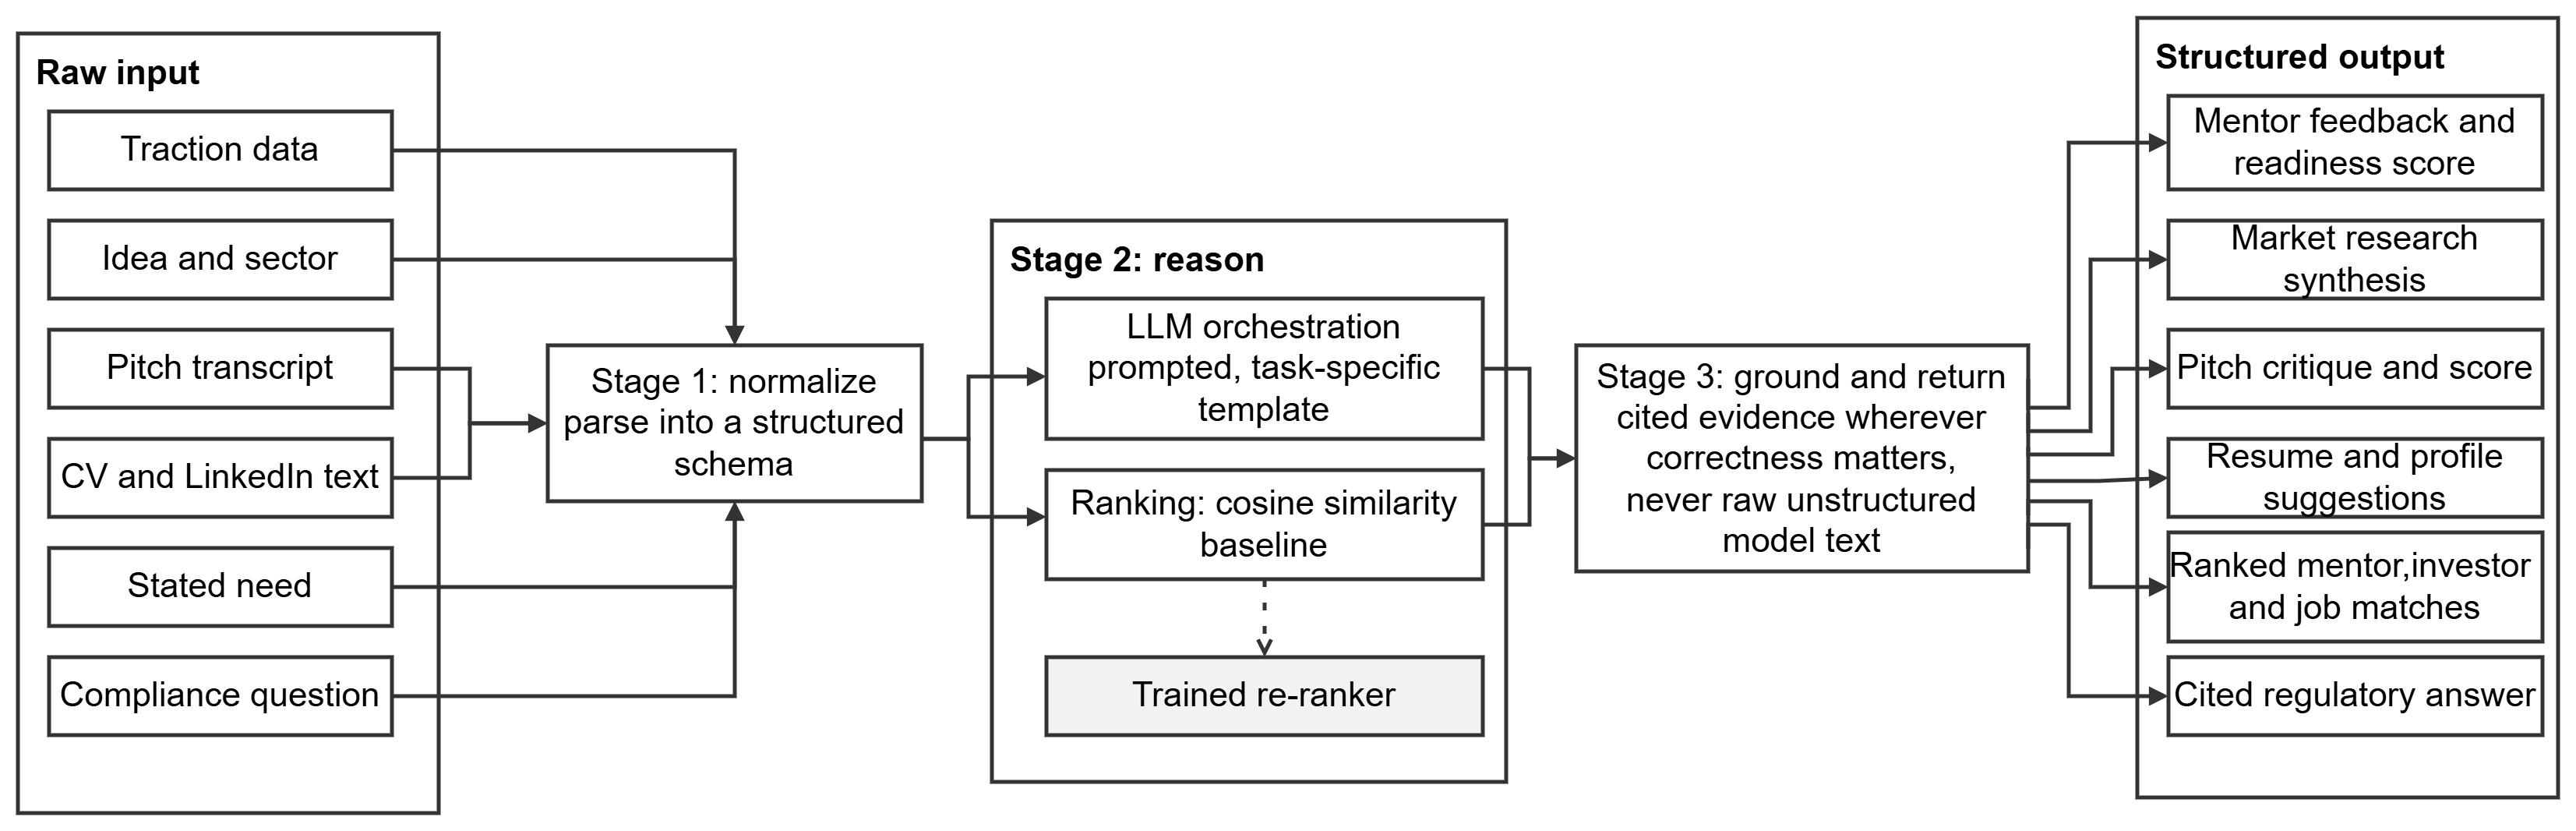
\includegraphics[width=\textwidth,height=1.0\textheight,keepaspectratio]{Figures/fig13_core_ai_engine.png}
\caption{Core AI reasoning engine}
\label{fig:core-engine}
\end{figure}

\section{Design Considerations}
The following section presents the problems that needed to be resolved prior to design. It includes assumptions and dependancies of the design, constraints that restrict it, goals that influenced it and the process it followed to create it. The majority of these problems are related to the “free-tier” setting and the small team outlined in Chapter~\ref{chap:vision}.

\subsection{Assumptions and Dependencies}
This design assumes availability of outside services. It is important to note that higher versions of the Gemini are not reliable under free tier load, so the platform is utilizing lower versions, which are called using one gateway and are around 5 calls at a time (NFR-2, NFR-19). If a student application is unable to obtain the LinkedIn API access, the other signals are used for verification and a greater number of applications are referred to a reviewer (FR-12). The trained reranker, Urdu and Roman Urdu support (FR-9), and a new model provider, are planned to come later and each will take one over an established boundary.

\subsection{General Constraints}
The free tiers on which the system is running determine the size of the system. It can support 50 users at a time (NFR-1) and approximately 5 model requests at a time; the remaining requests are placed in a queue. No local GPU required, since the embeddings are created in background jobs and there is no guarantee in regards to their availability. Only personal data is collected by opting in to register (NFR-9). The platform does not take equity, does not provide legal advice, as stated in Chapter~\ref{chap:vision}.

\subsection{Goals and Guidelines}\label{sec:goals-guidelines}
The design is guided by four goals. The first is that FYP-1 adopts the simplest strategy, as it can be compared with a simple baseline, before training; cosine similarity and feature weights. Second, when correctness is important, the system presents its evidence when it provides the answer, or it does not provide an answer. The third one would be that only the re-ranker is trained, which makes the training effort realistic for three developers. The fourth one is that every replaceable part has its own boundary, providers and models can change without rewriting.

\subsection{Development Methods}
The team operates in sprints where the foundations are delivered first, followed by the compliance assistant, matching and then the other prompted modules. Waterfall was rejected as some answers are not given till build, in the case of the corpus, with Rational Unified Process being too weighty for three developers. Changes in decisions are documented in a log with a date and changes to schema are versioned migrations (NFR-22). All pull requests need to be linted as part of the GitHub Actions workflow (NFR-23) and need to be approved by a different user to push code to the pull request.

\section{System Architecture}
The system is divided as shown in figure \ref{fig:architecture}. Each time the client requests the API gateway sends the request to one of the six services, and that service reads and writes the shared database. A language model is never called when it is matched. The other prompt features are only accessible via the LLM gateway, slow work runs in background via redis and celery. Services are split up by responsibility, so that each has its own owner and can be tested individually, but are deployed together, as described in Section~\ref{sec:strategies}.

\begin{figure}[H]
\centering
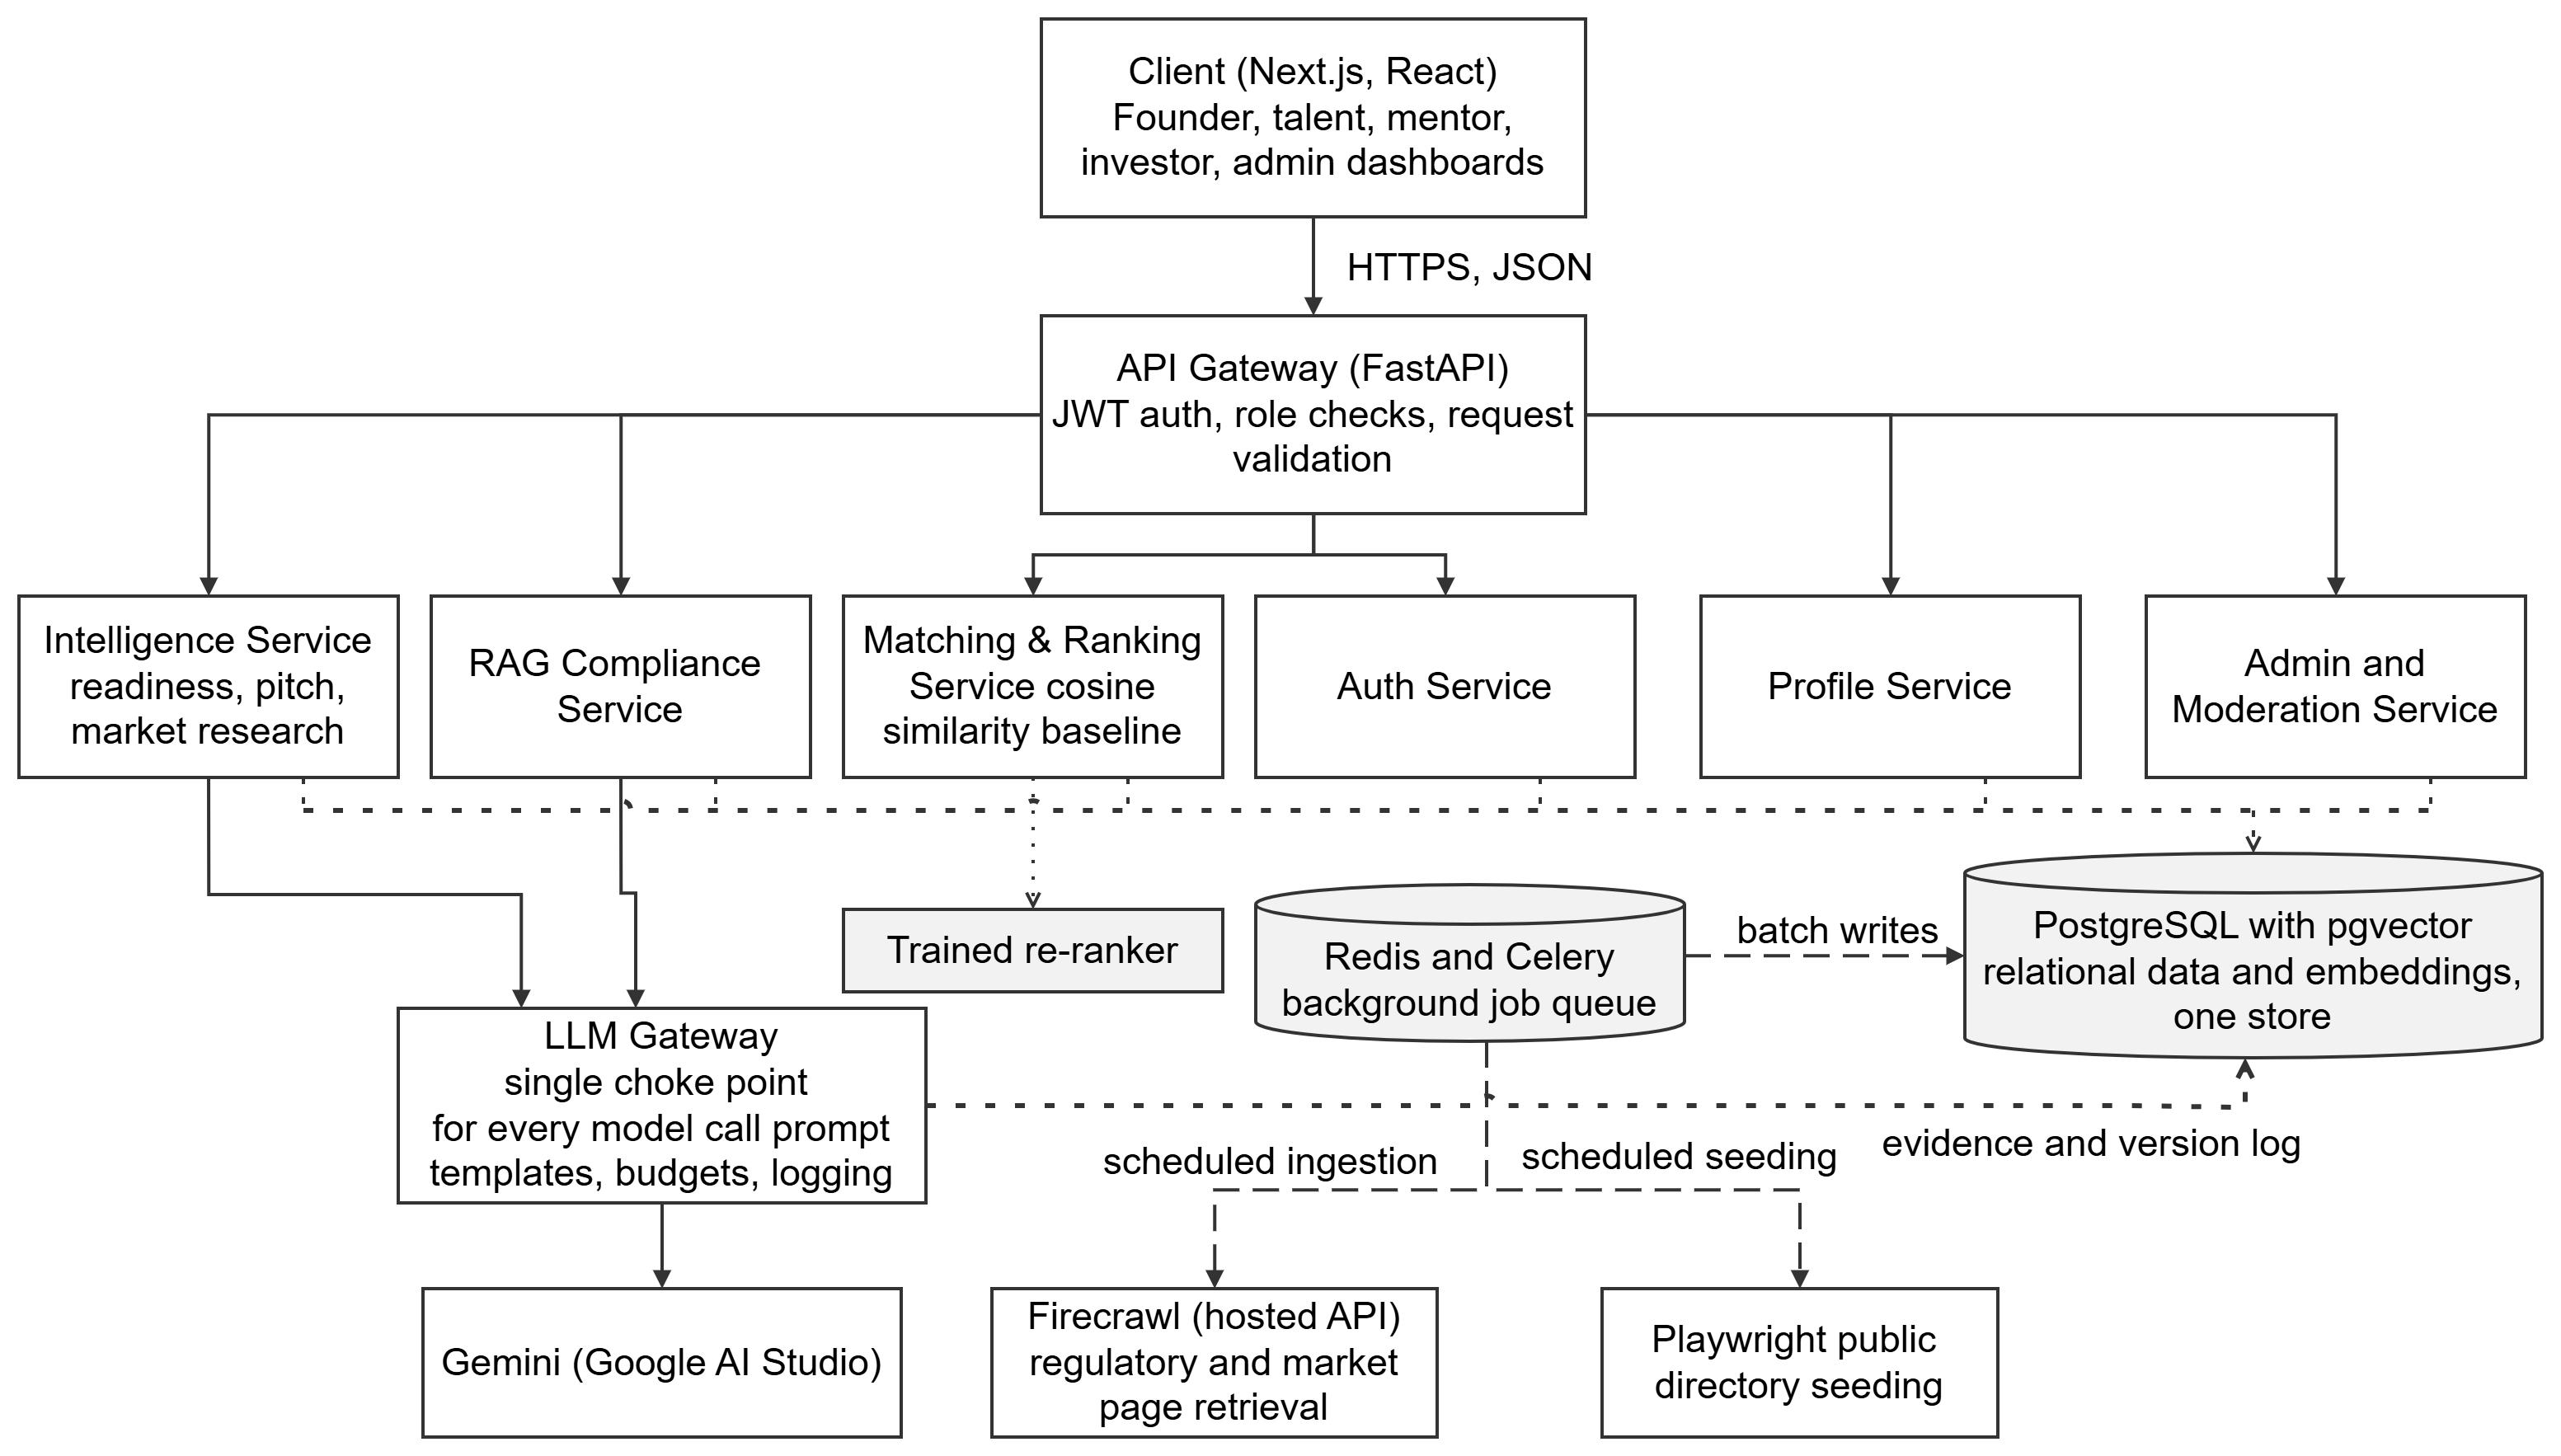
\includegraphics[width=\textwidth,height=0.88\textheight,keepaspectratio]{Figures/fig14_architecture_highlevel.png}
\caption{High-level system architecture}
\label{fig:architecture}
\end{figure}

\subsection{Subsystem Architecture}
The overview doesn't provide enough detail about four parts of the system. These include matching and ranking, retrieval and compliance, profile verification and a background pipeline. Matching and compliance are the most complicated flows, with each having their own diagram, and the other two are described in text. The description for each indicates what is constructed in FYP-1 and added in FYP-2.

\subsubsection{Matching and Ranking}
There are two phases of matching (Figure~\ref{fig:matching}). Stage 1 fetches the candidates by embedding similarity after hard filters which are all stored in Postgres using pgvector. For stage 2, a shortlist is ranked based on five factors (sector, stage, skills, availability and ticket fit) weighted by the cosine score. Once a human relevance set is available, this baseline will be replaced in FYP-2, when it is tested with NDCG@K and MRR and. Contact information will be shown after mutual acceptance.

\begin{figure}[H]
\centering
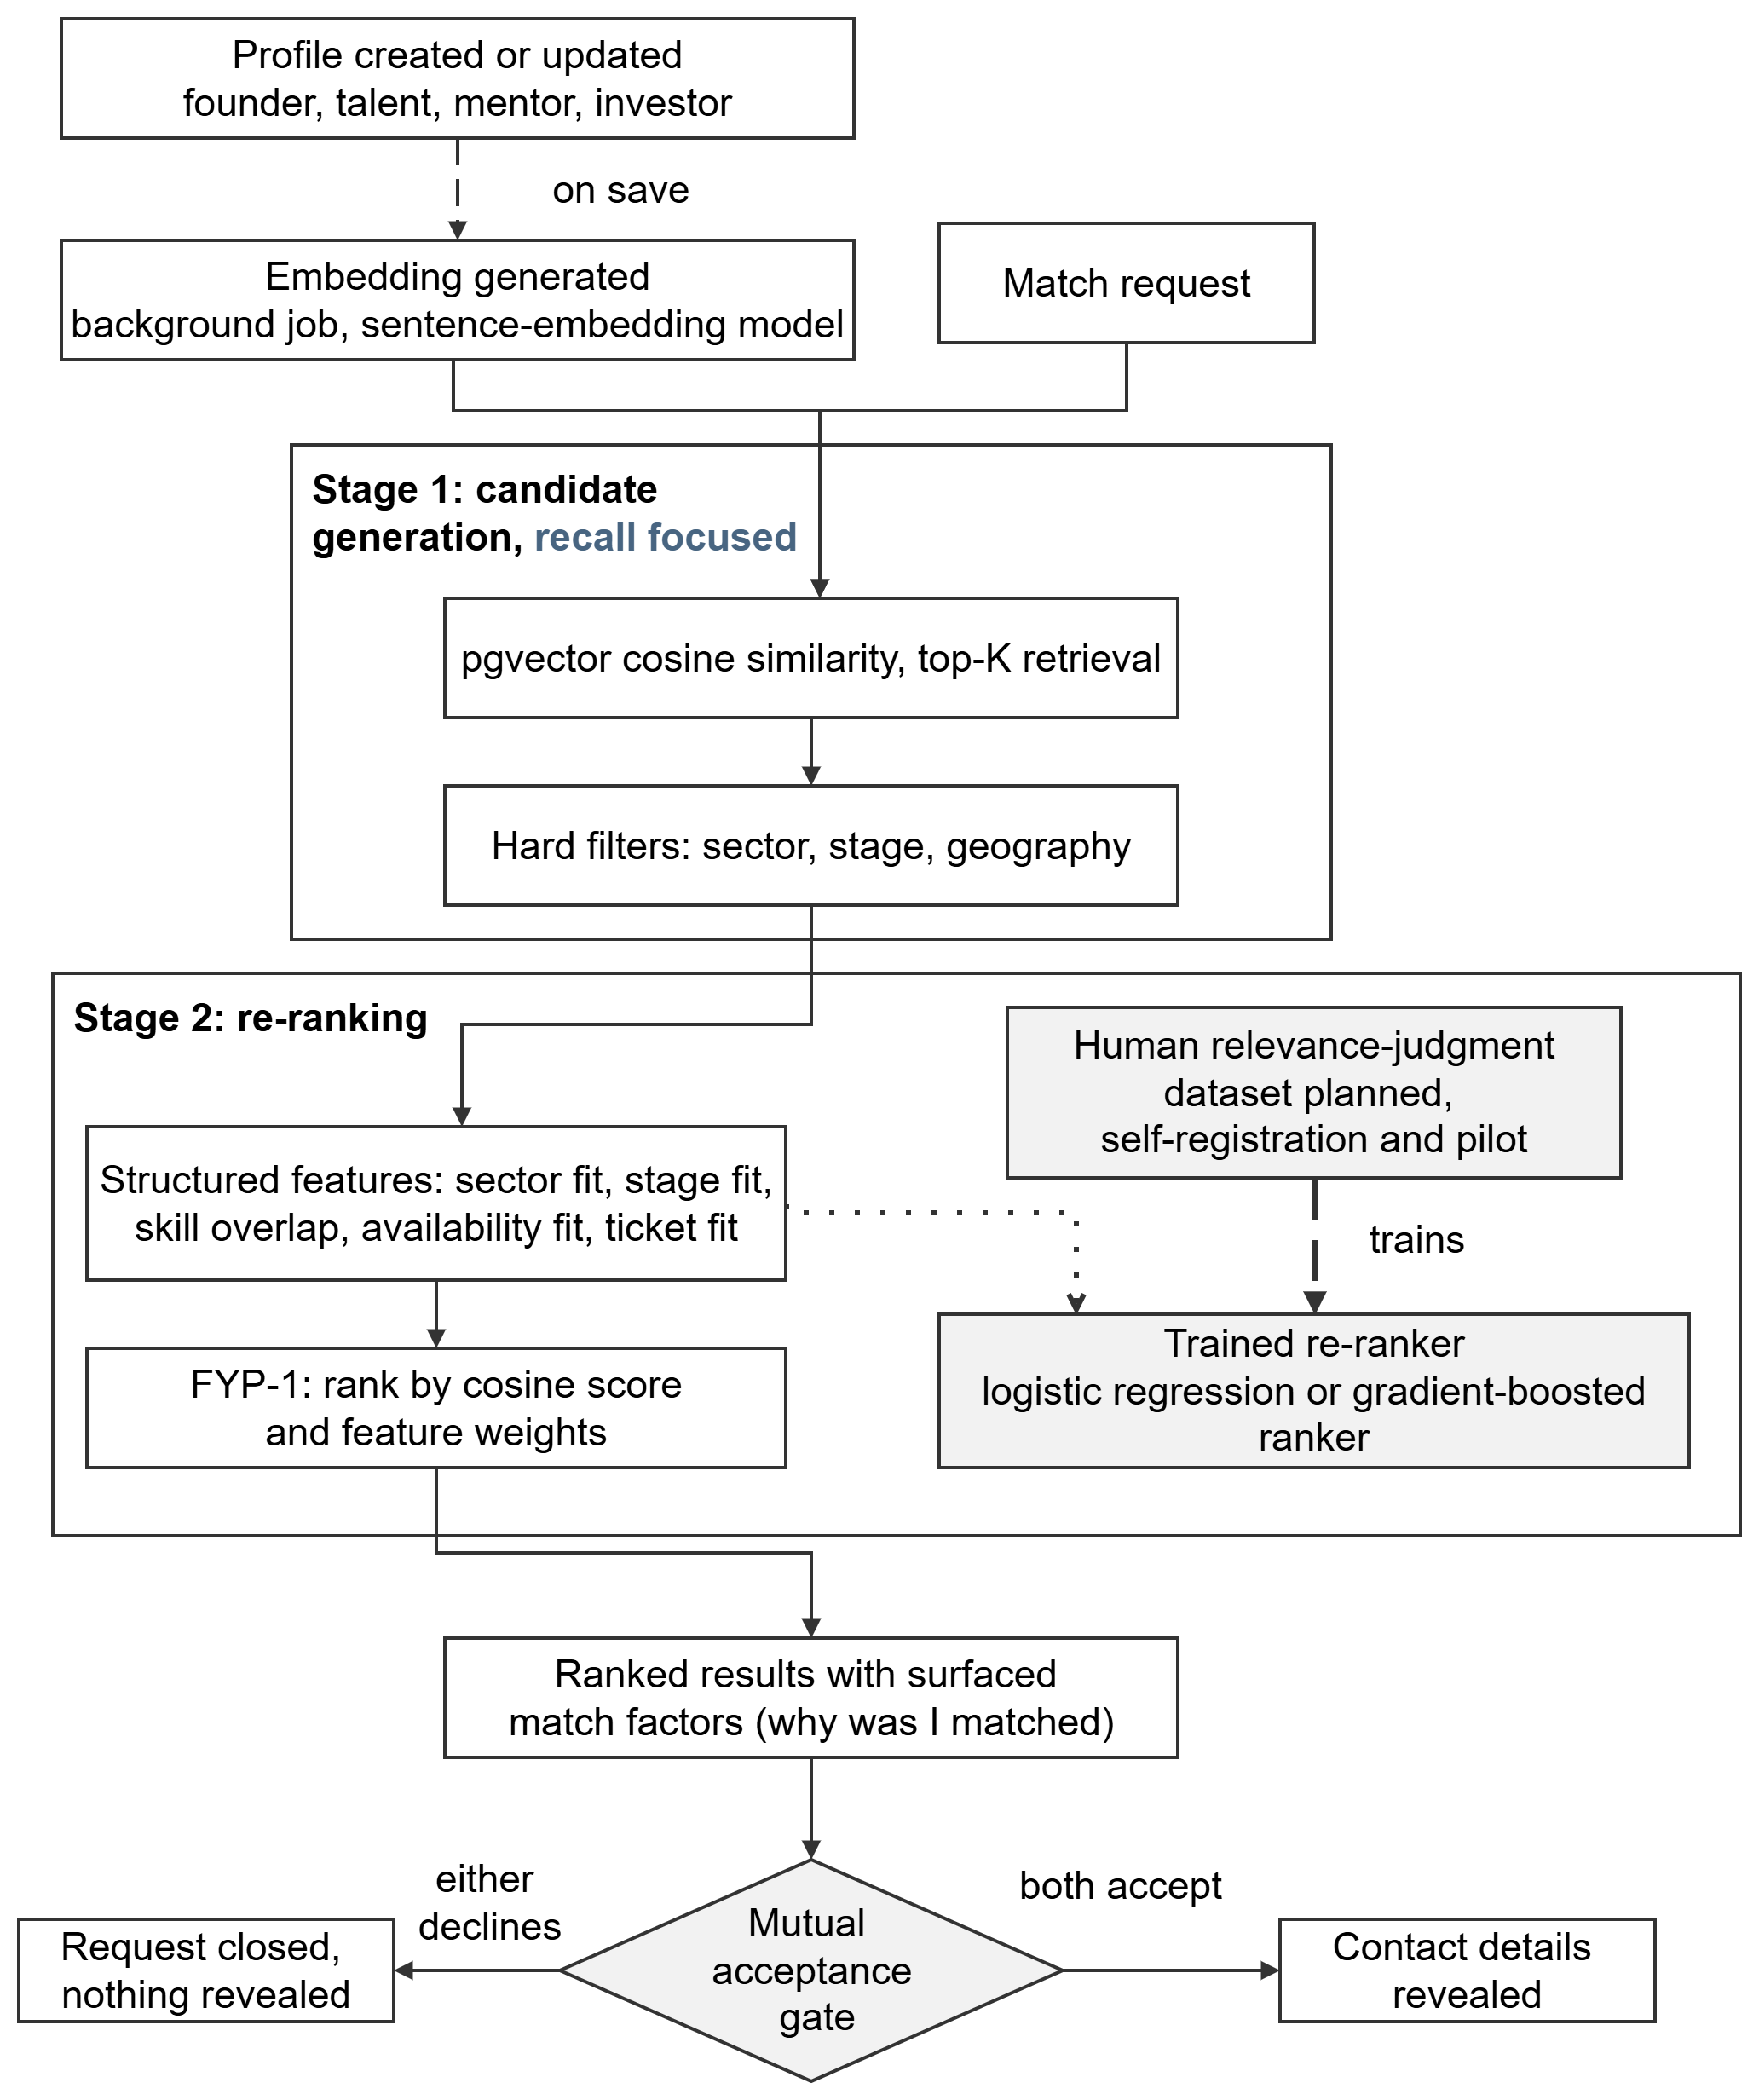
\includegraphics[width=\textwidth,height=0.7\textheight,keepaspectratio]{Figures/fig15_matching_subsystem.png}
\caption{Matching and ranking subsystem}
\label{fig:matching}
\end{figure}

\subsubsection{Retrieval and Compliance}
The assistant uses a hybrid approach to BM25 and dense retrieval, reciprocal rank fusion, and stores the top 5 passages of the corpus in PostgreSQL (Figure~\ref{fig:compliance}). It also rejects if the degree of similarity of the best passage is less than a threshold that was determined on the questions that were developed in advance of the test. If there is no passage that contains a corresponding answer, if validation fails, or if a case specific advice is requested, it will be declined. All queries are recorded with their answer, and refusing. There is no legal or tax advice provided in the answers.

\begin{figure}[H]
\centering
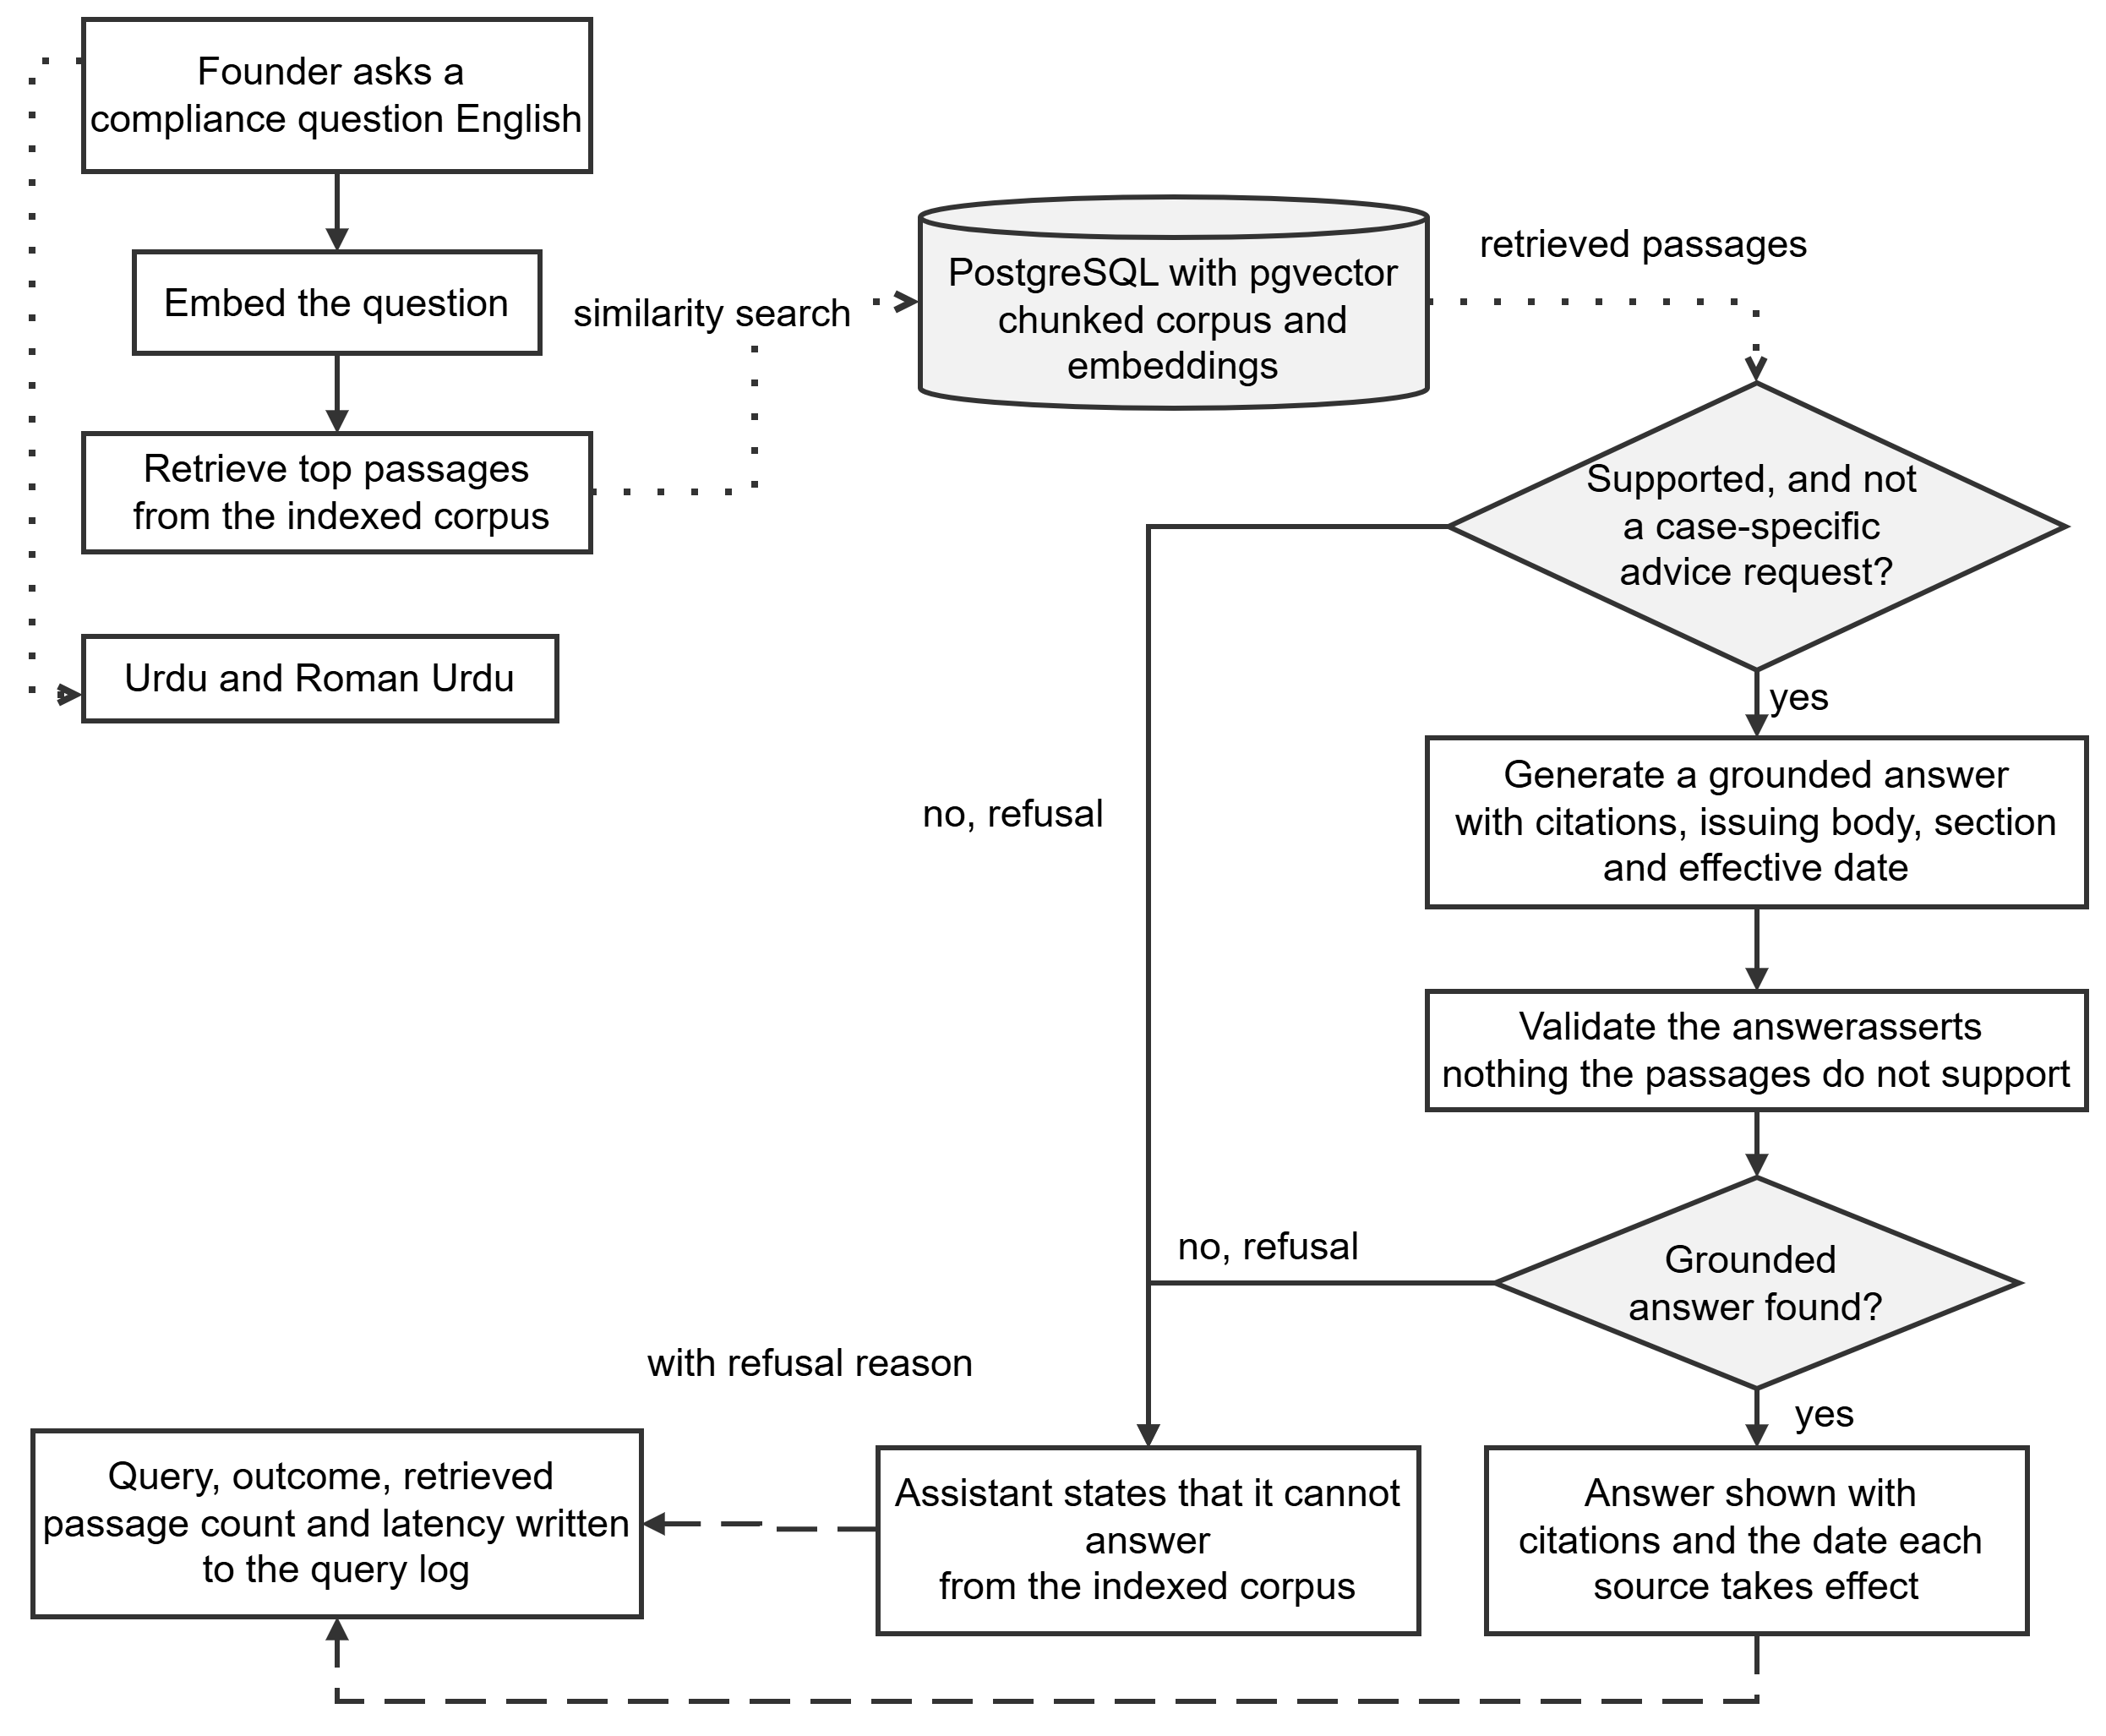
\includegraphics[width=\textwidth,height=0.7\textheight,keepaspectratio]{Figures/fig16_arch_compliance.png}
\caption{Compliance question flow with refusal path}
\label{fig:compliance}
\end{figure}

\subsubsection{Profile Verification}
A profile submission is automatically scored, based on 5 signals. These are the LinkedIn OAuth, SECP check, profile completeness, and GitHub activity for consistency between LinkedIn and a user's profile. The only call that is prompted is the link check; the other four calls are rules set by the team. A high score will be considered as an auto-verified profile while the check for SECP will remain a manual follow-up, a low score will be rejected and a middle score will be sent for human review (FR-14). If a user is rejected, he may appeal after submitting additional proof and the final decision on the appeal will be made by a reviewer.

\subsubsection{Background Pipeline}
The background jobs are run by celery and redis and output to a PostgreSQL. Using Firecrawl, whitelisted pages from SECP, FBR and PSEB are ingested and then chunked, embedded and indexed. Playwright posts his/her play about on public pages in the directory from public accelerator or incubator sites. Embeddings are re-generated when editing a profile and changes in embedding model. For FYP-2, a batch job trains the re-ranker; a new version is put into service only if it does not deviate from the cosine baseline.

\section{Architectural Strategies}\label{sec:strategies}
There are seven strategies for the architecture. A brief description of each follows along with the rationale for selection and rejection of the main alternative. Together they follow the goals in Section~\ref{sec:goals-guidelines} which are simplicity, evidence before answers and replaceable parts. The vast majority of them are formed by the restrictions of free tier and a group of three developers. The strategies are presented in order of those that affect the entire system to those that deal with faults and background work.

\subsection{Single LLM Gateway}
All LLM calls go through one internal gateway. It keeps the prompt templates, enforces the concurrency limit (NFR-2) and logs all calls; every assessment stored indicates the version of the prompt used to generate it. Then all a new provider has to do is a configuration change (NFR-19). The original suggestion was to call the model directly from each service, but this was turned down since the provider code and rate limits were distributed over 6 services, making them difficult to change.

\subsection{One Database with Vector Search}
Profiles, corpus records and embeddings are stored in one place in PostgreSQL with pgvector (NFR-20). A single query is able to filter the rows and also perform the vector search at our scale. A second vector database was rejected due to the necessity of having its own copy of the data, requiring additional synchronisation, and no benefit at the scale of this project. The profile embeddings will be stored in pgvector columns and the ranking will be based on Python function calls, a search is planned to be implemented in the database in FYP-2.

\subsection{Two-Stage Matching}
The candidates are selected by embedding similarity after hard filters, and re-ranked by a short list on structured features. The primary candidate is a LambdaMART ranker trained on the five factor scores, cosine score as well as features of the profile such as GitHub activity (FR-13). We selected it because boosted trees require only a few hundred labeled pairs to learn, train quickly and are able to explain why a pair is ranked high, whereas a cross-encoder could not be reliably trained with the 150-300 pairs we anticipate. The logistic regression, pointwise LightGBM and LambdaMART methods, and the simplest one (the winner) are compared on the same features.

\subsection{Grounded Generation with Refusal}
The compliance assistant gives only from retrieved passages, informs about the source and the date of its effectiveness (or about the date of the source if this is not provided) and denies when there is no answer in the corpus. A refined model was rejected since it is not able to refer to passages and the corpus can evolve over time. Finally, because commercial legal research tools hallucinated in the range of 17-33\% of the time \cite{ref:magesh2025} free answering was also rejected. If students do not answer, it is considered correct.

\subsection{Modular Services Deployed Together}
Services are split by responsibility, but are executed in a few container processes. A full separation of microservices was rejected as it was too much effort for the three developers, and one instance per microservice is not worth running on free microservice-hosting tiers. Matching and retrieval stay separated modules as they are very likely to be picked up later. This makes deployment easy at this point, and allows for scaling of those parts to be done separately.

\subsection{Background Tasks}
Slow operations are executed as a celery task on Redis. These are embedding, ingestion, directory seeding, link checks and in FYP-2 re-ranker training. Running them in the request will cause a failure in the response time and if the link check fails, it will prevent a profile from being submitted, so they weren't going to be running within the request. With background tasks. In case of failure, the failed tasks are retried and logged, and the rest of the queue will continue to run.

\subsection{Error Detection and Recovery}
If the concurrency is reached, requests are waiting in a queue and the interface displays them as being queued. If the model call fails, the results of the previous readiness assessment remain the same and the user can call the model again. If one of the verification signals is missing, the score uses the other signals and the profile is sent to a human verifier. It would not have been possible to fail entire request, as this would make it impossible to access when a free service is not available.

\section{Domain Model/Class Diagram}\label{sec:domain}
The Principal attributes, operations, associations and multiplicities of the ten principal classes of the domain model are displayed in Figure~\ref{fig:class-domain} of The Founder's Carnet. The data dictionary in Chapter~\ref{chap:software-requirements} gives the attributes of the matching database tables. Objects owned by an association are indicated with a filled Diamond, and thus are subject to the lifetime of their owner. The user contains the email, full name, role and active status. A user has startups with name, sector and stage. A startup's readiness assessments each have scores for 7 dimensions, and job listings, and applications are submitted by users for each job listing. A user enters verification cases with a computer-generated score and outcome and enters a decision/appeal status and assigns a reviewer to the cases the user reviews. A user also issues match requests, which are answered with ranked match results and also have explanations.

\begin{figure}[H]
\centering
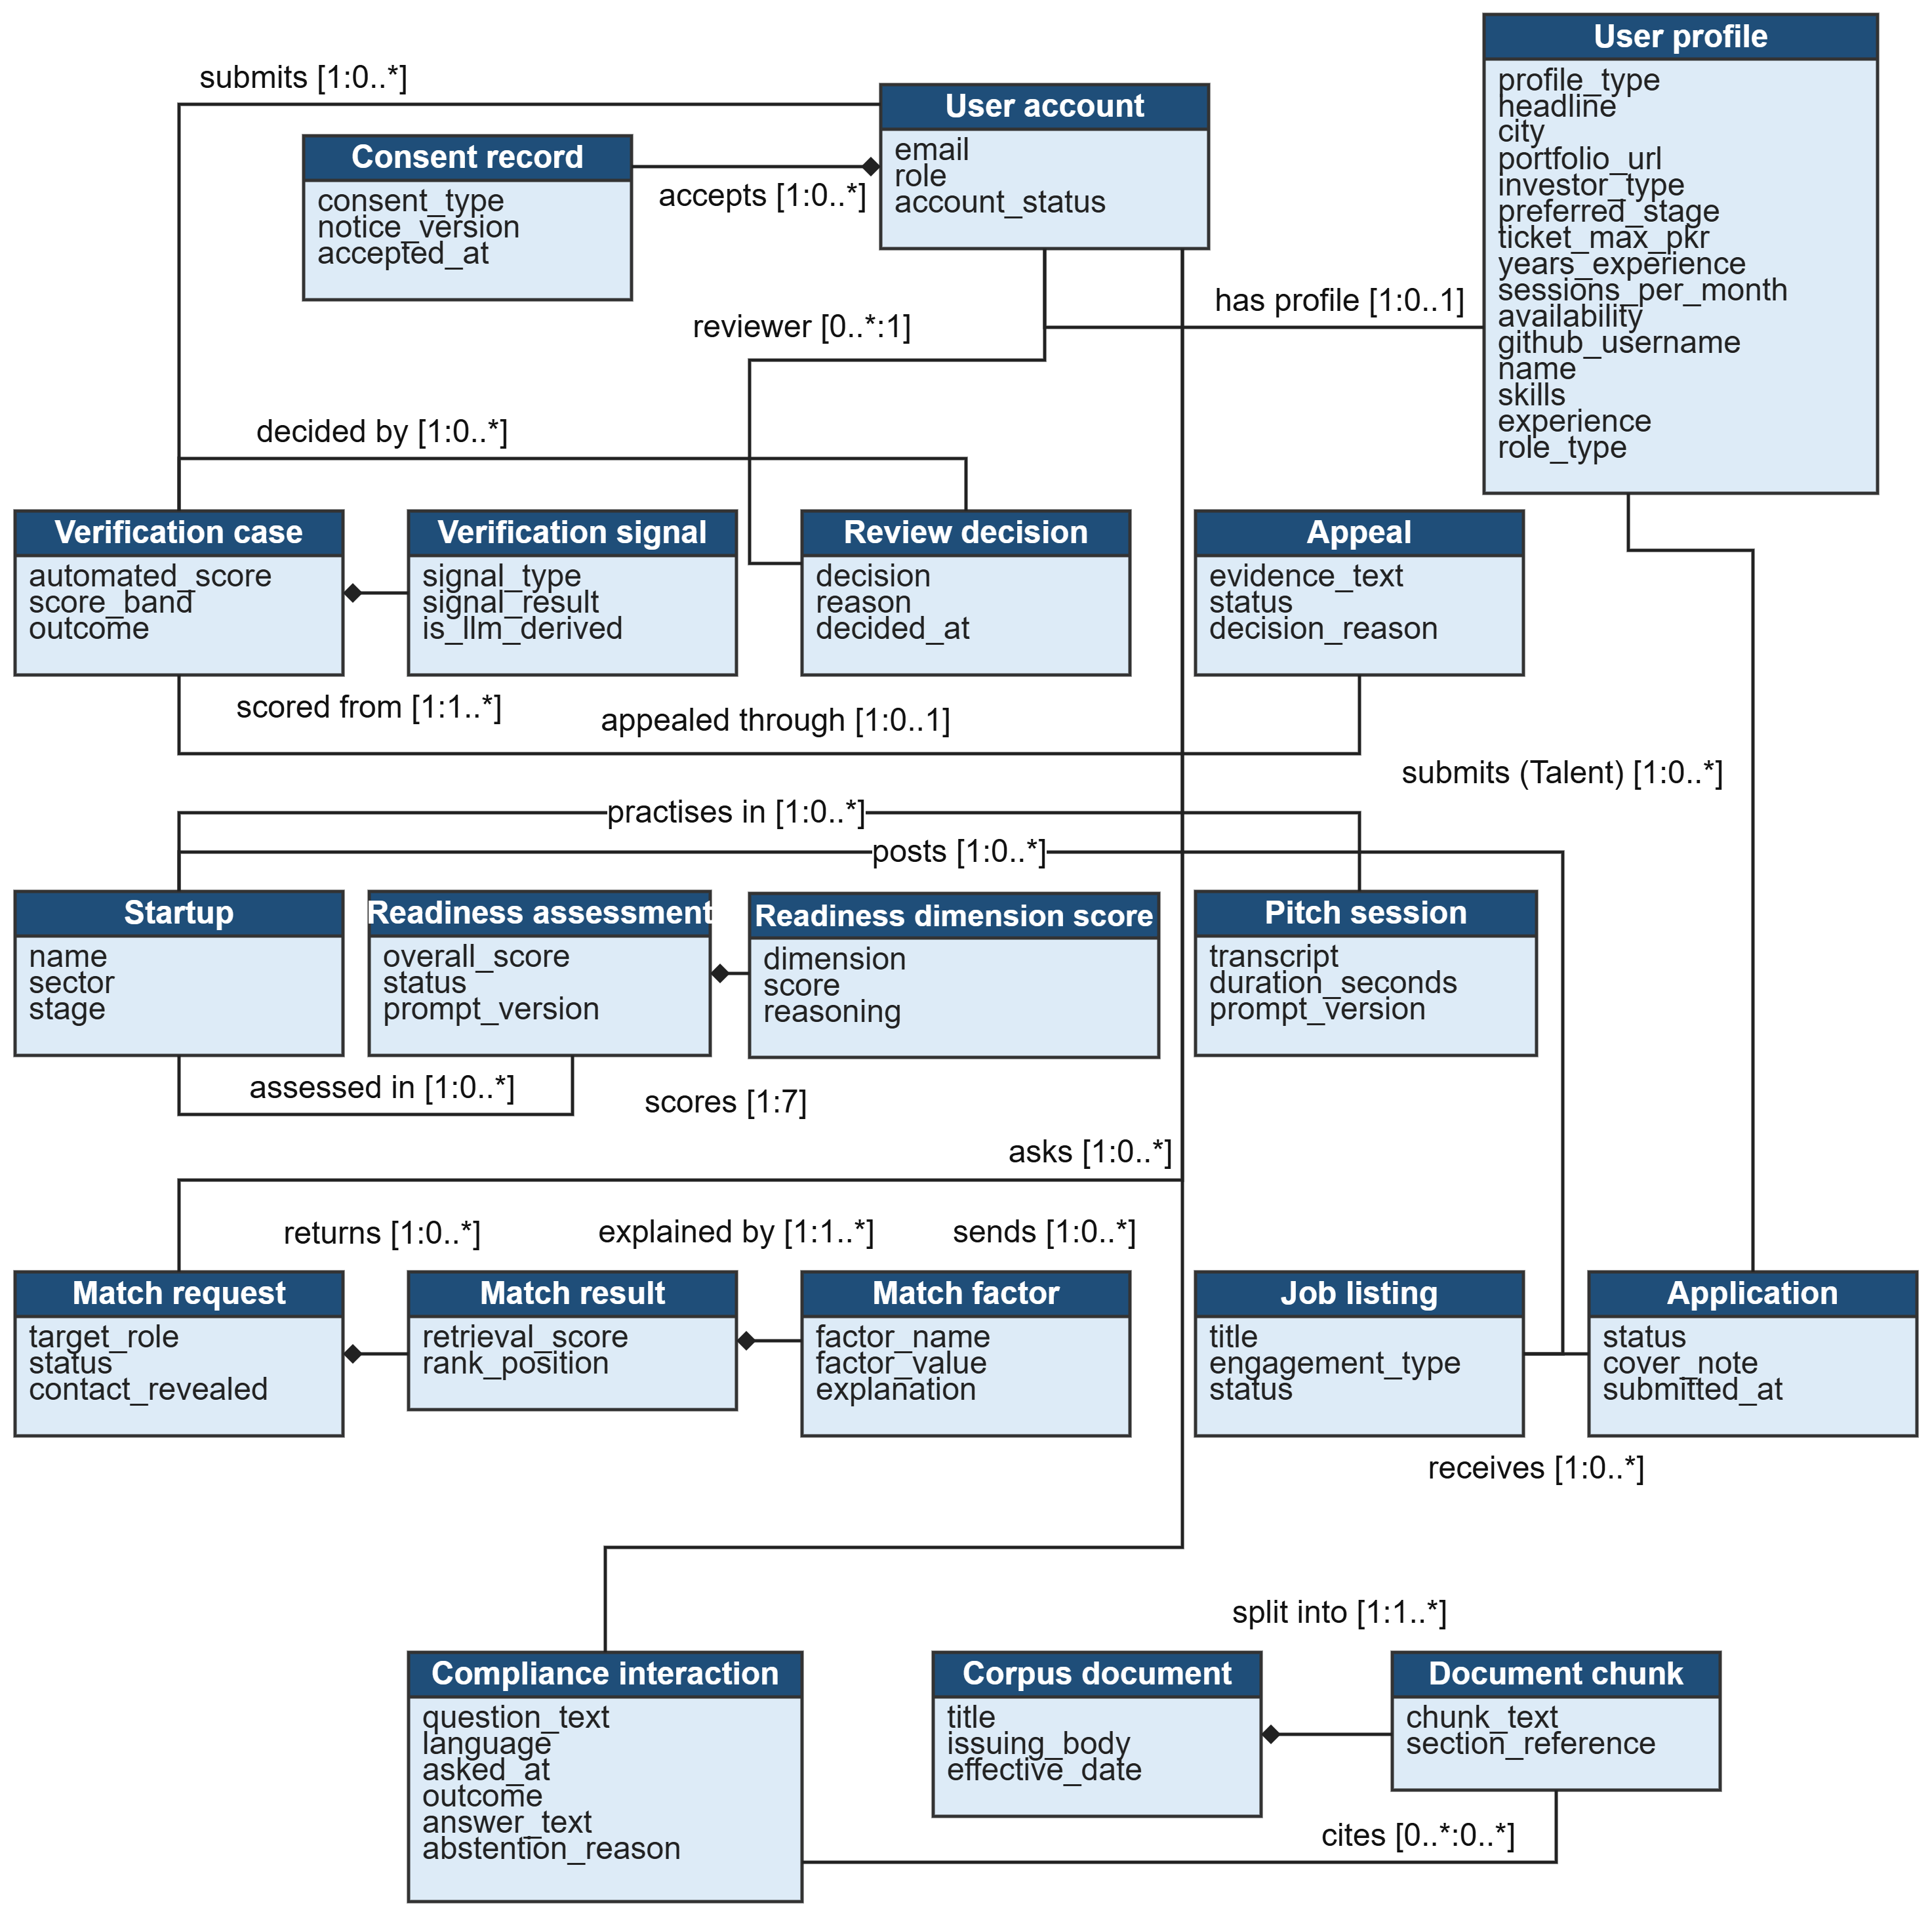
\includegraphics[width=\textwidth,height=0.88\textheight,keepaspectratio]{Figures/fig19_class_domain_model.png}
\caption{Class diagram of the domain model}
\label{fig:class-domain}
\end{figure}

\section{Policies and Tactics}\label{sec:dbchange}
This section discusses policies and tactics which do not alter the overall system structure, but are related to its construction, testing and release. A brief description of each with its reason is given. All 3 developers are included and will be automatically checked in the pipeline as long as possible. The code organization, quality gates, change management, configuration and security, and deployment policies described below are included.

\subsection{Code Organization}
The whole project is in one repository, with separate folders for the frontend, backend, rag and ml code, so a change across an API boundary is a single pull request. The back end is implemented in Python using typed request and response models and the front end is implemented in TypeScript. Multiple repositories were not accepted as multiple branches of the same functionality would end up in separate pull requests. This also means that each developer can test the entire project on a single clone, which tests the frontend, backend and retrieval code together.

\subsection{Quality Gates}
Linting does in fact run in the pull request pipeline and a failure prevents the pull request from being merged (NFR-23). In the unit tests, scoring and ranking is tested on known inputs. Integration tests include those that verify access control with no token, a token for the wrong role and before and after acceptance (NFR-5, NFR-6). Compliance assistant is also tested with a question set (hand-verified) for citations, recall and correct refusal. These checks are performed prior to the change being merged, thus a change to break access control behaviour or citation behaviour is detected before it reaches the main branch.

\subsection{Change Management}
Requirement IDs do not sequentially increase within their groups, since requirement IDs do not change. Versioned migrations are schema changes and the schema can be rebuilt from an empty database (NFR-22). Prompts, rubrics and corpus documents are versioned like code, and answers reference the date that a fee or rate is in effect (NFR-14). When requirement IDs, and the migration history are kept stable, a requirement and a test case can always be linked to a database change.

\subsection{Configuration and Security}
Credentials are provided in the pipeline configuration, and do not exist in the repository, and a pipeline step validates pull requests for API keys (NFR-8). The configurable values are the model provider, the model tier, the concurrency limits and the verification thresholds, so they can be changed without a code change. This also helps to prevent secrets from being added to the repository history, which is difficult to remove after it's committed.

\subsection{Deployment}
Docker Compose all services run locally. Frontend is deployed to Vercel from main branch, and backend is deployed to Railway or Render. The above platforms have been selected due to the availability of free tiers, which aligns with the budget mentioned in Chapter~\ref{chap:vision}. Docker Compose allows all three devs to have the same local environment, thereby eliminating the potential issues that might happen due to variations in machines.

\section{Conclusion}
This chapter gave an overview of the design of The Founder's Carnet. A Next.js client calls a FastAPI gateway that forwards requests to six services sharing one PostgreSQL database (with pgvector) and all model calls are routed through one LLM gateway. The matching and compliance subsystems were presented in this chapter with their diagrams, while the verification and background pipeline was presented in text. It described seven architectural strategies and the alternatives that were discarded, as well as the domain model of the system and its 10 core classes, and the policies used by the team. The matching re-ranker is a trained model (it is planned to be included in the FYP-2).

\chapter{Implementation and Test Cases}\label{ch:impl}
The prototype of the project built in FYP-1 and the tests conducted on them are described in this chapter. Section~\ref{sec:impl} provides a description of the platform as well as the six elements implemented. The eight test cases described in Section~\ref{sec:tcd} are presented in the template format and Section~\ref{sec:tm} provides the test metrics and how the requirements relate to the test cases. The prototype is a working back end with a web client that is not yet linked to the back end, and the screens are based on sample data. A conclusion is given at the end of the chapter about what is covered in the prototype and what remains for FYP-2.

\section{Implementation}\label{sec:impl}
Prototype is a working backend and not yet connected with a web client. The backend applies the components of the design in Section~\ref{sec:strategies} that require no labeled training data, and all requests to the language model go through one internal gateway (NFR-19). The following tools were used.
\begin{itemize}
\item Backend is implemented with Python 3.11, FastAPI, SQLAlchemy and Alembic migrations.
\item PostgreSQL 17 with pgvector extension for data and vector search
\item Setup Celery for background tasks and Redis for background tasks.
\item The language model is Gemini 2.5 Flash and the embedding model is multilingual-e5-base.
\item For the web client, the development tools used are Next.js, React and Tailwind CSS.
\item Using pytest and Playwright for tests, and GitHub Actions to do checks on every pull request.
\end{itemize}

\subsection{Accounts and Access}
A user registers (with an email, password and 1 role) and must accept to the user consent notice before registering (FR-17). You can't create an admin with a public registration, only by a command line script. All passwords are bcrypt–hashed with salted password, not shown in an error message (NFR-4) A login will return a signed token, which will be valid for 24 hours, all other endpoints will check the validity of the token and role (FR-23, NFR-5) and a logout cancels all prior logins. A user can withdraw his consent at any time and his account will be suspended immediately (FR-27) and his model answers will be deleted from the cache.

\subsection{Compliance Assistant}
The assistant must only respond from the official SECP, FBR and PSEB documents (FR-8). The documents are broken into sections and then paragraphs with document, page, section and effective date as citation data. The language model gateway supports 5 requests (NFR-2), retries a failure once, has a bounded timeout and only accepts answers with a schema. At step not failing to run (NFR-13), refused a question is addressed in the following steps.
\begin{enumerate}
\item Question asking whether user personally needs a licence or registration is refused as legal advice.
\item Five passages are found by hybrid search, which combines vector similarity and keyword ranking.
\item Question is refused ifS vector similarity is below 0.8428, a threshold tuned on development split.
\item Model answers with identifiers of passages it cites, and answer is refused if it cites a different one.
\item Answer is refused if a number or date is not in the cited passages, or if document has no date.
\item Second model call checks that the cited passages fully support the answer.
\end{enumerate}
An answer is provided as well as citations and a disclaimer that it is not legal or tax advice, followed by an answer and reason for refusal for each question.

\subsection{Profile Verification}
There are five signals which validate profiles of mentors, investors and talent: LinkedIn link, SECP cross-check, completeness of the profile, GitHub and portfolio link (FR-19, 20) consistency. The signal's weights are 0.03, 0.02, 0.65, 0.10 and 0.20, and are stored in a version controlled configuration file. The score ranges from 0.90+, automatically verified, 0.76, automatically rejected with a log reason, and everything in between is passed on to a human (FR-14). If a user is denied, he can provide more evidence for reconsideration. An admin will review the escalated profiles and appeals in a queue and document all decisions on the profile of the person who reviewed the profile and the reason (FR-21, 26). A profile which has been reported, or blocked, will go back to the review queue.

\subsection{Matching}
Matching is not based on a trained model. Only verified and open profiles within the same city will be stored, an investor will only be visible if the startup is verified and has a readiness assessment (FR-10, FR-29) A factor score is assigned to each profile: Sector fit (0.25), Stage fit (0.20), Skill overlap (0.25), Availability (0.15) and Ticket fit (0.15). This approach assigns a score to each match by averaging this factor score and the cosine similarity between the startup and profile text without needing any additional model call to explain each match (NFR-15). The weights: a first proposal, the contact details are hidden, until both parties agree (NFR-6), a background task refreshes a profile embedding when its text changes.

\subsection{Readiness Score and Pitch Practice}
The readiness score is based on a prompted model without the need for training data (FR-2). The model has to be repeated 7 times (problem clarity, market definition, differentiation, business model, traction, team and scalability; all must be between 1 and 5), the reasoning text has to be repeated 7 times, all the other answers are rejected, and it must have one next action, all other answers are rejected. All assessments are archived with the previous versions of the rubric and previous assessments are stored in the assessment history. In pitch practice, the simulated investor can only ask one follow up question per question pitched by the founders; scores are only awarded at the end of a pitch session (FR-3). In the event of a model call failure, the answer of the founder and the previous assessment is kept.

\subsection{Web Client}\label{sec:impl-frontend}
Based on the concept of Section~\ref{sec:gui}, the web client contains registration and login screens, as well as privacy and terms screens and a dashboard for each of the five types of users. The readiness dialog with the 7 dimensions, the pitch feedback and the match preview are visible on the founder dashboard. Currently, there is no screen connected to the backend and are populated with sample data. They are part of the plan for FYP-2 to connect them.

\section{Test Case Design and Description}\label{sec:tcd}
The behaviors of the prototype are tested and listed in the prototype requirements (Section~\ref{sec:fr}) in eight test cases. Two test backend, two test web client and four test other components. Automated pytest and Playwright tests are used to run the backend and the web client test cases. The following attributes are common to all test cases.
\begin{itemize}
\item PostgreSQL with pgvector is not part of all backend test cases, which are run using Python 3.11, pytest 8.3.4, and an in memory SQL database.
\item Language and embedding model are replaced by fixed test doubles and tests reflect not the quality of language or embedding model, but how the application uses the model answers.
\item The test cases are independent of each other as they produce their own users and data.
\item All test cases were tested on 18 November 2026 and team performed the task as testers and reviewers in turn.
\end{itemize}

\begin{table}[!ht]
\caption{Test case No.1: Registration, Login and Logout}
\label{tab:tc1}
\centering
\small
\setlength{\tabcolsep}{3pt}
\renewcommand{\arraystretch}{1.25}
\begin{tabular}{|>{\raggedright\arraybackslash}p{0.21\textwidth}|>{\raggedright\arraybackslash}p{0.25\textwidth}|>{\raggedright\arraybackslash}p{0.19\textwidth}|>{\raggedright\arraybackslash}p{0.20\textwidth}|}
\hline
\multicolumn{4}{|c|}{\textbf{Accounts and Access Module}} \\ \hline
\multicolumn{4}{|c|}{\textbf{FR-17, FR-22, FR-23, NFR-4, NFR-5}} \\ \hline
\textbf{Test Case ID:} & \textit{1} & \textbf{QA Test Engineer:} & \textit{Ali Ahmad} \\ \hline
\textbf{Test case Version:} & \textit{1} & \textbf{Reviewed By:} & \textit{Shahzeb Imran} \\ \hline
\textbf{Test Date:} & \textit{22-11-2026} & \textbf{Use Case Reference(s):} & \textit{Table~\ref{tab:uc-register}} \\ \hline
\textbf{Revision History:} & \multicolumn{3}{>{\raggedright\arraybackslash}p{\dimexpr .64\textwidth+4\tabcolsep\relax}|}{\textit{None}} \\ \hline
\textbf{Objective:} & \multicolumn{3}{>{\raggedright\arraybackslash}p{\dimexpr .64\textwidth+4\tabcolsep\relax}|}{\textit{Test registration, login and logout.}} \\ \hline
\textbf{Product/Ver/ Module:} & \multicolumn{3}{>{\raggedright\arraybackslash}p{\dimexpr .64\textwidth+4\tabcolsep\relax}|}{\textit{Backend, authentication.}} \\ \hline
\textbf{Environment:} & \multicolumn{3}{>{\raggedright\arraybackslash}p{\dimexpr .64\textwidth+4\tabcolsep\relax}|}{\textit{Python 3.11, pytest, SQLite.}} \\ \hline
\textbf{Assumptions:} & \multicolumn{3}{>{\raggedright\arraybackslash}p{\dimexpr .64\textwidth+4\tabcolsep\relax}|}{\textit{None.}} \\ \hline
\textbf{Pre-Requisite:} & \multicolumn{3}{>{\raggedright\arraybackslash}p{\dimexpr .64\textwidth+4\tabcolsep\relax}|}{\textit{None.}} \\ \hline
\textbf{Step No.} & \textbf{Execution description} & \multicolumn{2}{>{\raggedright\arraybackslash}p{\dimexpr .39\textwidth+2\tabcolsep\relax}|}{\textbf{Procedure result}} \\ \hline
1 & \textit{Register with consent.} & \multicolumn{2}{>{\raggedright\arraybackslash}p{\dimexpr .39\textwidth+2\tabcolsep\relax}|}{\textit{Account created.}} \\ \hline
2 & \textit{Register as admin.} & \multicolumn{2}{>{\raggedright\arraybackslash}p{\dimexpr .39\textwidth+2\tabcolsep\relax}|}{\textit{Rejected.}} \\ \hline
3 & \textit{Submit an invalid password.} & \multicolumn{2}{>{\raggedright\arraybackslash}p{\dimexpr .39\textwidth+2\tabcolsep\relax}|}{\textit{Error, password not shown.}} \\ \hline
4 & \textit{Login with correct details.} & \multicolumn{2}{>{\raggedright\arraybackslash}p{\dimexpr .39\textwidth+2\tabcolsep\relax}|}{\textit{Token returned.}} \\ \hline
5 & \textit{Logout, reuse old token.} & \multicolumn{2}{>{\raggedright\arraybackslash}p{\dimexpr .39\textwidth+2\tabcolsep\relax}|}{\textit{Token rejected.}} \\ \hline
\multicolumn{4}{|l|}{\textbf{Comments:} \textit{All steps passed.}} \\ \hline
\multicolumn{4}{|c|}{\textbf{\underline{Passed}}\qquad \textit{Failed}\qquad \textit{Not Executed}} \\ \hline
\end{tabular}
\end{table}


\begin{table}[!ht]
\caption{Test case No.2: Mobile Layout of the Public Screens}
\label{tab:tc2}
\centering
\small
\setlength{\tabcolsep}{3pt}
\renewcommand{\arraystretch}{1.25}
\begin{tabular}{|>{\raggedright\arraybackslash}p{0.21\textwidth}|>{\raggedright\arraybackslash}p{0.25\textwidth}|>{\raggedright\arraybackslash}p{0.19\textwidth}|>{\raggedright\arraybackslash}p{0.20\textwidth}|}
\hline
\multicolumn{4}{|c|}{\textbf{Web Client Module}} \\ \hline
\multicolumn{4}{|c|}{\textbf{NFR-16}} \\ \hline
\textbf{Test Case ID:} & \textit{4} & \textbf{QA Test Engineer:} & \textit{Ali Ahmad} \\ \hline
\textbf{Test case Version:} & \textit{1} & \textbf{Reviewed By:} & \textit{Taha Nawaz} \\ \hline
\textbf{Test Date:} & \textit{22-11-2026} & \textbf{Use Case Reference(s):} & \textit{None} \\ \hline
\textbf{Revision History:} & \multicolumn{3}{>{\raggedright\arraybackslash}p{\dimexpr .64\textwidth+4\tabcolsep\relax}|}{\textit{None}} \\ \hline
\textbf{Objective:} & \multicolumn{3}{>{\raggedright\arraybackslash}p{\dimexpr .64\textwidth+4\tabcolsep\relax}|}{\textit{Test public screens fit 390px without horizontal scroll.}} \\ \hline
\textbf{Product/Ver/ Module:} & \multicolumn{3}{>{\raggedright\arraybackslash}p{\dimexpr .64\textwidth+4\tabcolsep\relax}|}{\textit{Web client, public pages.}} \\ \hline
\textbf{Environment:} & \multicolumn{3}{>{\raggedright\arraybackslash}p{\dimexpr .64\textwidth+4\tabcolsep\relax}|}{\textit{Playwright test, viewport 390x844 px.}} \\ \hline
\textbf{Assumptions:} & \multicolumn{3}{>{\raggedright\arraybackslash}p{\dimexpr .64\textwidth+4\tabcolsep\relax}|}{\textit{None.}} \\ \hline
\textbf{Pre-Requisite:} & \multicolumn{3}{>{\raggedright\arraybackslash}p{\dimexpr .64\textwidth+4\tabcolsep\relax}|}{\textit{Web client running on localhost:3000.}} \\ \hline
\textbf{Step No.} & \textbf{Execution description} & \multicolumn{2}{>{\raggedright\arraybackslash}p{\dimexpr .39\textwidth+2\tabcolsep\relax}|}{\textbf{Procedure result}} \\ \hline
1 & \textit{Open landing, login, register, privacy, terms screens.} & \multicolumn{2}{>{\raggedright\arraybackslash}p{\dimexpr .39\textwidth+2\tabcolsep\relax}|}{\textit{Every screen loads with status 200.}} \\ \hline
2 & \textit{Compare scroll width.} & \multicolumn{2}{>{\raggedright\arraybackslash}p{\dimexpr .39\textwidth+2\tabcolsep\relax}|}{\textit{No screen wider than 390 px.}} \\ \hline
3 & \textit{Try scrolling sideways.} & \multicolumn{2}{>{\raggedright\arraybackslash}p{\dimexpr .39\textwidth+2\tabcolsep\relax}|}{\textit{Horizontal position unchanged.}} \\ \hline
\multicolumn{4}{|l|}{\textbf{Comments:} \textit{All steps passed.}} \\ \hline
\multicolumn{4}{|c|}{\textbf{\underline{Passed}}\qquad \textit{Failed}\qquad \textit{Not Executed}} \\ \hline
\end{tabular}
\end{table}

\begin{table}[!ht]
\caption{Test case No.3: Appeal Decision by an Admin}
\label{tab:tc3}
\centering
\small
\setlength{\tabcolsep}{3pt}
\renewcommand{\arraystretch}{1.25}
\begin{tabular}{|>{\raggedright\arraybackslash}p{0.21\textwidth}|>{\raggedright\arraybackslash}p{0.25\textwidth}|>{\raggedright\arraybackslash}p{0.19\textwidth}|>{\raggedright\arraybackslash}p{0.20\textwidth}|}
\hline
\multicolumn{4}{|c|}{\textbf{Profile Verification Module}} \\ \hline
\multicolumn{4}{|c|}{\textbf{FR-15, FR-21, FR-26, NFR-5}} \\ \hline
\textbf{Test Case ID:} & \textit{2} & \textbf{QA Test Engineer:} & \textit{Shahzeb Imran} \\ \hline
\textbf{Test case Version:} & \textit{1} & \textbf{Reviewed By:} & \textit{Taha Nawaz} \\ \hline
\textbf{Test Date:} & \textit{22-11-2026} & \textbf{Use Case Reference(s):} & \textit{Table~\ref{tab:uc-appeal}} \\ \hline
\textbf{Revision History:} & \multicolumn{3}{>{\raggedright\arraybackslash}p{\dimexpr .64\textwidth+4\tabcolsep\relax}|}{\textit{None}} \\ \hline
\textbf{Objective:} & \multicolumn{3}{>{\raggedright\arraybackslash}p{\dimexpr .64\textwidth+4\tabcolsep\relax}|}{\textit{Test single appeal and recorded admin decision.}} \\ \hline
\textbf{Product/Ver/ Module:} & \multicolumn{3}{>{\raggedright\arraybackslash}p{\dimexpr .64\textwidth+4\tabcolsep\relax}|}{\textit{Backend prototype, verification and admin review.}} \\ \hline
\textbf{Environment:} & \multicolumn{3}{>{\raggedright\arraybackslash}p{\dimexpr .64\textwidth+4\tabcolsep\relax}|}{\textit{Python 3.11, pytest 8.3.4, in-memory SQLite.}} \\ \hline
\textbf{Assumptions:} & \multicolumn{3}{>{\raggedright\arraybackslash}p{\dimexpr .64\textwidth+4\tabcolsep\relax}|}{\textit{Portfolio check result supplied by test.}} \\ \hline
\textbf{Pre-Requisite:} & \multicolumn{3}{>{\raggedright\arraybackslash}p{\dimexpr .64\textwidth+4\tabcolsep\relax}|}{\textit{Investor profile with inconsistent portfolio check.}} \\ \hline
\textbf{Step No.} & \textbf{Execution description} & \multicolumn{2}{>{\raggedright\arraybackslash}p{\dimexpr .39\textwidth+2\tabcolsep\relax}|}{\textbf{Procedure result}} \\ \hline
1 & \textit{Investor appeals with reason and evidence.} & \multicolumn{2}{>{\raggedright\arraybackslash}p{\dimexpr .39\textwidth+2\tabcolsep\relax}|}{\textit{Appeal saved.}} \\ \hline
2 & \textit{Admin opens review queue.} & \multicolumn{2}{>{\raggedright\arraybackslash}p{\dimexpr .39\textwidth+2\tabcolsep\relax}|}{\textit{Shows appeal pending with evidence.}} \\ \hline
3 & \textit{Admin approves with reason.} & \multicolumn{2}{>{\raggedright\arraybackslash}p{\dimexpr .39\textwidth+2\tabcolsep\relax}|}{\textit{Status changes to verified.}} \\ \hline
4 & \textit{Investor checks own status.} & \multicolumn{2}{>{\raggedright\arraybackslash}p{\dimexpr .39\textwidth+2\tabcolsep\relax}|}{\textit{Status is verified.}} \\ \hline
5 & \textit{Check stored decision.} & \multicolumn{2}{>{\raggedright\arraybackslash}p{\dimexpr .39\textwidth+2\tabcolsep\relax}|}{\textit{Reviewer and reason saved.}} \\ \hline
\multicolumn{4}{|l|}{\textbf{Comments:} \textit{All steps passed.}} \\ \hline
\multicolumn{4}{|c|}{\textbf{\underline{Passed}}\qquad \textit{Failed}\qquad \textit{Not Executed}} \\ \hline
\end{tabular}
\end{table}


\begin{table}[!ht]
\caption{Test case No.4: Consent on the Registration Screen}
\label{tab:tc4}
\centering
\small
\setlength{\tabcolsep}{3pt}
\renewcommand{\arraystretch}{1.25}
\begin{tabular}{|>{\raggedright\arraybackslash}p{0.21\textwidth}|>{\raggedright\arraybackslash}p{0.25\textwidth}|>{\raggedright\arraybackslash}p{0.19\textwidth}|>{\raggedright\arraybackslash}p{0.20\textwidth}|}
\hline
\multicolumn{4}{|c|}{\textbf{Web Client Module}} \\ \hline
\multicolumn{4}{|c|}{\textbf{FR-17}} \\ \hline
\textbf{Test Case ID:} & \textit{3} & \textbf{QA Test Engineer:} & \textit{Taha Nawaz} \\ \hline
\textbf{Test case Version:} & \textit{1} & \textbf{Reviewed By:} & \textit{Ali Ahmad} \\ \hline
\textbf{Test Date:} & \textit{22-11-2026} & \textbf{Use Case Reference(s):} & \textit{Table~\ref{tab:uc-register}} \\ \hline
\textbf{Revision History:} & \multicolumn{3}{>{\raggedright\arraybackslash}p{\dimexpr .64\textwidth+4\tabcolsep\relax}|}{\textit{None}} \\ \hline
\textbf{Objective:} & \multicolumn{3}{>{\raggedright\arraybackslash}p{\dimexpr .64\textwidth+4\tabcolsep\relax}|}{\textit{Test registration blocked until consent ticked.}} \\ \hline
\textbf{Product/Ver/ Module:} & \multicolumn{3}{>{\raggedright\arraybackslash}p{\dimexpr .64\textwidth+4\tabcolsep\relax}|}{\textit{Web client, registration screen.}} \\ \hline
\textbf{Environment:} & \multicolumn{3}{>{\raggedright\arraybackslash}p{\dimexpr .64\textwidth+4\tabcolsep\relax}|}{\textit{Playwright test against Next.js dev server.}} \\ \hline
\textbf{Assumptions:} & \multicolumn{3}{>{\raggedright\arraybackslash}p{\dimexpr .64\textwidth+4\tabcolsep\relax}|}{\textit{Backend not called.}} \\ \hline
\textbf{Pre-Requisite:} & \multicolumn{3}{>{\raggedright\arraybackslash}p{\dimexpr .64\textwidth+4\tabcolsep\relax}|}{\textit{Web client running on localhost:3000.}} \\ \hline
\textbf{Step No.} & \textbf{Execution description} & \multicolumn{2}{>{\raggedright\arraybackslash}p{\dimexpr .39\textwidth+2\tabcolsep\relax}|}{\textbf{Procedure result}} \\ \hline
1 & \textit{Open registration screen.} & \multicolumn{2}{>{\raggedright\arraybackslash}p{\dimexpr .39\textwidth+2\tabcolsep\relax}|}{\textit{Consent unticked, Create account disabled.}} \\ \hline
2 & \textit{Enter email and password only.} & \multicolumn{2}{>{\raggedright\arraybackslash}p{\dimexpr .39\textwidth+2\tabcolsep\relax}|}{\textit{Create account stays disabled.}} \\ \hline
3 & \textit{Tick consent box.} & \multicolumn{2}{>{\raggedright\arraybackslash}p{\dimexpr .39\textwidth+2\tabcolsep\relax}|}{\textit{Create account enabled, notice disappears.}} \\ \hline
4 & \textit{Untick consent box.} & \multicolumn{2}{>{\raggedright\arraybackslash}p{\dimexpr .39\textwidth+2\tabcolsep\relax}|}{\textit{Create account disabled again.}} \\ \hline
\multicolumn{4}{|l|}{\textbf{Comments:} \textit{All steps passed.}} \\ \hline
\multicolumn{4}{|c|}{\textbf{\underline{Passed}}\qquad \textit{Failed}\qquad \textit{Not Executed}} \\ \hline
\end{tabular}
\end{table}


\begin{table}[!ht]
\caption{Test case No.5: Embedding Regeneration Task}
\label{tab:tc5}
\centering
\small
\setlength{\tabcolsep}{3pt}
\renewcommand{\arraystretch}{1.25}
\begin{tabular}{|>{\raggedright\arraybackslash}p{0.21\textwidth}|>{\raggedright\arraybackslash}p{0.25\textwidth}|>{\raggedright\arraybackslash}p{0.19\textwidth}|>{\raggedright\arraybackslash}p{0.20\textwidth}|}
\hline
\multicolumn{4}{|c|}{\textbf{Background Tasks Module}} \\ \hline
\multicolumn{4}{|c|}{\textbf{FR-7, NFR-20}} \\ \hline
\textbf{Test Case ID:} & \textit{8} & \textbf{QA Test Engineer:} & \textit{Shahzeb Imran} \\ \hline
\textbf{Test case Version:} & \textit{1} & \textbf{Reviewed By:} & \textit{Taha Nawaz} \\ \hline
\textbf{Test Date:} & \textit{22-11-2026} & \textbf{Use Case Reference(s):} & \textit{None} \\ \hline
\textbf{Revision History:} & \multicolumn{3}{>{\raggedright\arraybackslash}p{\dimexpr .64\textwidth+4\tabcolsep\relax}|}{\textit{None}} \\ \hline
\textbf{Objective:} & \multicolumn{3}{>{\raggedright\arraybackslash}p{\dimexpr .64\textwidth+4\tabcolsep\relax}|}{\textit{Test task refreshes only out-of-date embeddings.}} \\ \hline
\textbf{Product/Ver/ Module:} & \multicolumn{3}{>{\raggedright\arraybackslash}p{\dimexpr .64\textwidth+4\tabcolsep\relax}|}{\textit{Backend prototype, Celery tasks.}} \\ \hline
\textbf{Environment:} & \multicolumn{3}{>{\raggedright\arraybackslash}p{\dimexpr .64\textwidth+4\tabcolsep\relax}|}{\textit{Python 3.11, pytest 8.3.4, in-memory SQLite.}} \\ \hline
\textbf{Assumptions:} & \multicolumn{3}{>{\raggedright\arraybackslash}p{\dimexpr .64\textwidth+4\tabcolsep\relax}|}{\textit{Tasks run directly, no worker or Redis started.}} \\ \hline
\textbf{Pre-Requisite:} & \multicolumn{3}{>{\raggedright\arraybackslash}p{\dimexpr .64\textwidth+4\tabcolsep\relax}|}{\textit{Profile without embedding exists.}} \\ \hline
\textbf{Step No.} & \textbf{Execution description} & \multicolumn{2}{>{\raggedright\arraybackslash}p{\dimexpr .39\textwidth+2\tabcolsep\relax}|}{\textbf{Procedure result}} \\ \hline
1 & \textit{Run task for new profile.} & \multicolumn{2}{>{\raggedright\arraybackslash}p{\dimexpr .39\textwidth+2\tabcolsep\relax}|}{\textit{Result updated.}} \\ \hline
2 & \textit{Run task again, no change.} & \multicolumn{2}{>{\raggedright\arraybackslash}p{\dimexpr .39\textwidth+2\tabcolsep\relax}|}{\textit{Result skipped.}} \\ \hline
3 & \textit{Change summary, run batch task.} & \multicolumn{2}{>{\raggedright\arraybackslash}p{\dimexpr .39\textwidth+2\tabcolsep\relax}|}{\textit{One profile updated, none skipped.}} \\ \hline
4 & \textit{Count embedding model calls.} & \multicolumn{2}{>{\raggedright\arraybackslash}p{\dimexpr .39\textwidth+2\tabcolsep\relax}|}{\textit{Model called twice in total.}} \\ \hline
\multicolumn{4}{|l|}{\textbf{Comments:} \textit{All steps passed.}} \\ \hline
\multicolumn{4}{|c|}{\textbf{\underline{Passed}}\qquad \textit{Failed}\qquad \textit{Not Executed}} \\ \hline
\end{tabular}
\end{table}


\begin{table}[!ht]
\caption{Test case No.6: Compliance Answer and Refusal}
\label{tab:tc6}
\centering
\small
\setlength{\tabcolsep}{3pt}
\renewcommand{\arraystretch}{1.25}
\begin{tabular}{|>{\raggedright\arraybackslash}p{0.21\textwidth}|>{\raggedright\arraybackslash}p{0.25\textwidth}|>{\raggedright\arraybackslash}p{0.19\textwidth}|>{\raggedright\arraybackslash}p{0.20\textwidth}|}
\hline
\multicolumn{4}{|c|}{\textbf{Compliance Assistant Module}} \\ \hline
\multicolumn{4}{|c|}{\textbf{FR-8, NFR-12, NFR-13}} \\ \hline
\textbf{Test Case ID:} & \textit{5} & \textbf{QA Test Engineer:} & \textit{Shahzeb Imran} \\ \hline
\textbf{Test case Version:} & \textit{1} & \textbf{Reviewed By:} & \textit{Ali Ahmad} \\ \hline
\textbf{Test Date:} & \textit{22-11-2026} & \textbf{Use Case Reference(s):} & \textit{Table~\ref{tab:uc-refuse}} \\ \hline
\textbf{Revision History:} & \multicolumn{3}{>{\raggedright\arraybackslash}p{\dimexpr .64\textwidth+4\tabcolsep\relax}|}{\textit{None}} \\ \hline
\textbf{Objective:} & \multicolumn{3}{>{\raggedright\arraybackslash}p{\dimexpr .64\textwidth+4\tabcolsep\relax}|}{\textit{Test cited answers vs refusal.}} \\ \hline
\textbf{Product/Ver/ Module:} & \multicolumn{3}{>{\raggedright\arraybackslash}p{\dimexpr .64\textwidth+4\tabcolsep\relax}|}{\textit{Backend prototype, compliance assistant.}} \\ \hline
\textbf{Environment:} & \multicolumn{3}{>{\raggedright\arraybackslash}p{\dimexpr .64\textwidth+4\tabcolsep\relax}|}{\textit{Python 3.11, pytest 8.3.4, in-memory SQLite.}} \\ \hline
\textbf{Assumptions:} & \multicolumn{3}{>{\raggedright\arraybackslash}p{\dimexpr .64\textwidth+4\tabcolsep\relax}|}{\textit{LM and embedding model replaced by test doubles.}} \\ \hline
\textbf{Pre-Requisite:} & \multicolumn{3}{>{\raggedright\arraybackslash}p{\dimexpr .64\textwidth+4\tabcolsep\relax}|}{\textit{Test corpus of passages stored.}} \\ \hline
\textbf{Step No.} & \textbf{Execution description} & \multicolumn{2}{>{\raggedright\arraybackslash}p{\dimexpr .39\textwidth+2\tabcolsep\relax}|}{\textbf{Procedure result}} \\ \hline
1 & \textit{Ask a stored passage supports.} & \multicolumn{2}{>{\raggedright\arraybackslash}p{\dimexpr .39\textwidth+2\tabcolsep\relax}|}{\textit{Answer saved with citation.}} \\ \hline
2 & \textit{Ask if needs SECP license.} & \multicolumn{2}{>{\raggedright\arraybackslash}p{\dimexpr .39\textwidth+2\tabcolsep\relax}|}{\textit{Refuses without embedding/model call.}} \\ \hline
3 & \textit{Ask unrelated question.} & \multicolumn{2}{>{\raggedright\arraybackslash}p{\dimexpr .39\textwidth+2\tabcolsep\relax}|}{\textit{Refuses without model call.}} \\ \hline
4 & \textit{Model cites non-retrieved passage.} & \multicolumn{2}{>{\raggedright\arraybackslash}p{\dimexpr .39\textwidth+2\tabcolsep\relax}|}{\textit{Answer refused.}} \\ \hline
\multicolumn{4}{|l|}{\textbf{Comments:} \textit{All steps passed.}} \\ \hline
\multicolumn{4}{|c|}{\textbf{\underline{Passed}}\qquad \textit{Failed}\qquad \textit{Not Executed}} \\ \hline
\end{tabular}
\end{table}


\begin{table}[!ht]
\caption{Test case No.7: Matching and Contact Reveal}
\label{tab:tc7}
\centering
\small
\setlength{\tabcolsep}{3pt}
\renewcommand{\arraystretch}{1.25}
\begin{tabular}{|>{\raggedright\arraybackslash}p{0.21\textwidth}|>{\raggedright\arraybackslash}p{0.25\textwidth}|>{\raggedright\arraybackslash}p{0.19\textwidth}|>{\raggedright\arraybackslash}p{0.20\textwidth}|}
\hline
\multicolumn{4}{|c|}{\textbf{Matching Module}} \\ \hline
\multicolumn{4}{|c|}{\textbf{FR-7, FR-10, FR-29, NFR-6, NFR-15}} \\ \hline
\textbf{Test Case ID:} & \textit{6} & \textbf{QA Test Engineer:} & \textit{Taha Nawaz} \\ \hline
\textbf{Test case Version:} & \textit{1} & \textbf{Reviewed By:} & \textit{Shahzeb Imran} \\ \hline
\textbf{Test Date:} & \textit{22-11-2026} & \textbf{Use Case Reference(s):} & \textit{Table~\ref{tab:uc-match}} \\ \hline
\textbf{Revision History:} & \multicolumn{3}{>{\raggedright\arraybackslash}p{\dimexpr .64\textwidth+4\tabcolsep\relax}|}{\textit{None}} \\ \hline
\textbf{Objective:} & \multicolumn{3}{>{\raggedright\arraybackslash}p{\dimexpr .64\textwidth+4\tabcolsep\relax}|}{\textit{Test hard filters and mutual-consent contact reveal.}} \\ \hline
\textbf{Product/Ver/ Module:} & \multicolumn{3}{>{\raggedright\arraybackslash}p{\dimexpr .64\textwidth+4\tabcolsep\relax}|}{\textit{Backend prototype, matching module.}} \\ \hline
\textbf{Environment:} & \multicolumn{3}{>{\raggedright\arraybackslash}p{\dimexpr .64\textwidth+4\tabcolsep\relax}|}{\textit{Python 3.11, pytest 8.3.4, in-memory SQLite.}} \\ \hline
\textbf{Assumptions:} & \multicolumn{3}{>{\raggedright\arraybackslash}p{\dimexpr .64\textwidth+4\tabcolsep\relax}|}{\textit{Embeddings from fixed test double.}} \\ \hline
\textbf{Pre-Requisite:} & \multicolumn{3}{>{\raggedright\arraybackslash}p{\dimexpr .64\textwidth+4\tabcolsep\relax}|}{\textit{Founder with startup and three verified mentors exist.}} \\ \hline
\textbf{Step No.} & \textbf{Execution description} & \multicolumn{2}{>{\raggedright\arraybackslash}p{\dimexpr .39\textwidth+2\tabcolsep\relax}|}{\textbf{Procedure result}} \\ \hline
1 & \textit{Request matches; one mentor in Karachi.} & \multicolumn{2}{>{\raggedright\arraybackslash}p{\dimexpr .39\textwidth+2\tabcolsep\relax}|}{\textit{Only open Lahore mentor returned.}} \\ \hline
2 & \textit{Read returned match.} & \multicolumn{2}{>{\raggedright\arraybackslash}p{\dimexpr .39\textwidth+2\tabcolsep\relax}|}{\textit{Shows five factors and score, no contact email.}} \\ \hline
3 & \textit{Mentor accepts match.} & \multicolumn{2}{>{\raggedright\arraybackslash}p{\dimexpr .39\textwidth+2\tabcolsep\relax}|}{\textit{Status pending, contact hidden.}} \\ \hline
4 & \textit{Founder accepts match.} & \multicolumn{2}{>{\raggedright\arraybackslash}p{\dimexpr .39\textwidth+2\tabcolsep\relax}|}{\textit{Contact details of both sides shown.}} \\ \hline
\multicolumn{4}{|l|}{\textbf{Comments:} \textit{All steps passed.}} \\ \hline
\multicolumn{4}{|c|}{\textbf{\underline{Passed}}\qquad \textit{Failed}\qquad \textit{Not Executed}} \\ \hline
\end{tabular}
\end{table}


\begin{table}[!ht]
\caption{Test case No.8: Readiness Score Validation}
\label{tab:tc8}
\centering
\small
\setlength{\tabcolsep}{3pt}
\renewcommand{\arraystretch}{1.25}
\begin{tabular}{|>{\raggedright\arraybackslash}p{0.21\textwidth}|>{\raggedright\arraybackslash}p{0.25\textwidth}|>{\raggedright\arraybackslash}p{0.19\textwidth}|>{\raggedright\arraybackslash}p{0.20\textwidth}|}
\hline
\multicolumn{4}{|c|}{\textbf{Readiness Score Module}} \\ \hline
\multicolumn{4}{|c|}{\textbf{FR-2, NFR-15}} \\ \hline
\textbf{Test Case ID:} & \textit{7} & \textbf{QA Test Engineer:} & \textit{Ali Ahmad} \\ \hline
\textbf{Test case Version:} & \textit{1} & \textbf{Reviewed By:} & \textit{Taha Nawaz} \\ \hline
\textbf{Test Date:} & \textit{22-11-2026} & \textbf{Use Case Reference(s):} & \textit{Table~\ref{tab:uc-readiness}} \\ \hline
\textbf{Revision History:} & \multicolumn{3}{>{\raggedright\arraybackslash}p{\dimexpr .64\textwidth+4\tabcolsep\relax}|}{\textit{None}} \\ \hline
\textbf{Objective:} & \multicolumn{3}{>{\raggedright\arraybackslash}p{\dimexpr .64\textwidth+4\tabcolsep\relax}|}{\textit{Test only complete, valid answers stored as assessment.}} \\ \hline
\textbf{Product/Ver/ Module:} & \multicolumn{3}{>{\raggedright\arraybackslash}p{\dimexpr .64\textwidth+4\tabcolsep\relax}|}{\textit{Readiness package and backend endpoint.}} \\ \hline
\textbf{Environment:} & \multicolumn{3}{>{\raggedright\arraybackslash}p{\dimexpr .64\textwidth+4\tabcolsep\relax}|}{\textit{Python 3.11, pytest 8.3.4, in-memory SQLite.}} \\ \hline
\textbf{Assumptions:} & \multicolumn{3}{>{\raggedright\arraybackslash}p{\dimexpr .64\textwidth+4\tabcolsep\relax}|}{\textit{LM replaced by fixed answers.}} \\ \hline
\textbf{Pre-Requisite:} & \multicolumn{3}{>{\raggedright\arraybackslash}p{\dimexpr .64\textwidth+4\tabcolsep\relax}|}{\textit{Founder and startup exist.}} \\ \hline
\textbf{Step No.} & \textbf{Execution description} & \multicolumn{2}{>{\raggedright\arraybackslash}p{\dimexpr .39\textwidth+2\tabcolsep\relax}|}{\textbf{Procedure result}} \\ \hline
1 & \textit{Answer with all seven dimensions.} & \multicolumn{2}{>{\raggedright\arraybackslash}p{\dimexpr .39\textwidth+2\tabcolsep\relax}|}{\textit{Stored with scores, reasoning, rubric version.}} \\ \hline
2 & \textit{Missing or repeated dimension.} & \multicolumn{2}{>{\raggedright\arraybackslash}p{\dimexpr .39\textwidth+2\tabcolsep\relax}|}{\textit{Rejected.}} \\ \hline
3 & \textit{Score outside range 1-5.} & \multicolumn{2}{>{\raggedright\arraybackslash}p{\dimexpr .39\textwidth+2\tabcolsep\relax}|}{\textit{Rejected.}} \\ \hline
4 & \textit{Model call fails.} & \multicolumn{2}{>{\raggedright\arraybackslash}p{\dimexpr .39\textwidth+2\tabcolsep\relax}|}{\textit{Previous assessment kept.}} \\ \hline
\multicolumn{4}{|l|}{\textbf{Comments:} \textit{All steps passed.}} \\ \hline
\multicolumn{4}{|c|}{\textbf{\underline{Passed}}\qquad \textit{Failed}\qquad \textit{Not Executed}} \\ \hline
\end{tabular}
\end{table}

\FloatBarrier

\section{Test Metrics}\label{sec:tm}
The values of the metrics of the eight test cases are presented in Table~\ref{tab:results} and the link between each requirement and test cases is presented as a traceability matrix. Effectiveness is not specified since no defect was found.

\begin{table}[!ht]
\centering
\caption{Test case Metric No.1}
\label{tab:results}
\small
\setlength{\tabcolsep}{3pt}
\renewcommand{\arraystretch}{1.25}
\begin{tabular}{|>{\raggedright\arraybackslash}p{.28\textwidth}|>{\raggedright\arraybackslash}p{.62\textwidth}|}
\hline
\textbf{Metric} & \textbf{Value} \\ \hline
\textbf{Number of Test Cases} & 8 \\ \hline
\textbf{Number of Test Cases Passed} & 8 \\ \hline
\textbf{Number of Test Cases Failed} & 0 \\ \hline
\textbf{Test Case Defect Density} & 0\% \\ \hline
\textbf{Test Case Effectiveness} & Not defined (0 defects detected) \\ \hline
\textbf{Traceability Matrix} & The eight test cases cover FR-2, 7, 8, 10, 15, 17, 21, 22, 23, 26, 29 and NFR-4, 5, 6, 12, 13, 15, 16, 20. Each requirement is listed in the header of its test case. \\ \hline
\end{tabular}
\end{table}

\subsection{Test Case Metric No.2}
The eight test cases are part of the automated suites of the project, whose size and result are given in Table~\ref{tab:suite}.

\begin{table}[!ht]
\centering
\caption{Test case Metric No.2}
\label{tab:suite}
\small
\setlength{\tabcolsep}{3pt}
\renewcommand{\arraystretch}{1.25}
\begin{tabular}{|l|c|c|c|}
\hline
\textbf{Part of the system} & \textbf{Tests} & \textbf{Passed} & \textbf{Failed} \\ \hline
Backend (pytest) & 164 & 164 & 0 \\ \hline
Retrieval package (pytest) & 63 & 63 & 0 \\ \hline
Readiness package (pytest) & 10 & 10 & 0 \\ \hline
Web client (Playwright) & 20 & 20 & 0 \\ \hline
\textbf{Total} & \textbf{257} & \textbf{257} & \textbf{0} \\ \hline
\end{tabular}
\end{table}


\section{Conclusion}
The prototype implements the parts of the platform that do not depend on labeled data, which are accounts and roles, the compliance assistant, profile verification, the matching baseline, the readiness score with the pitch practice, and the screens of the web client. All 8 test cases and all 257 automated tests passed, so the defect density of this run is 0\%. This result has limits. The backend tests use test doubles for the models and an in-memory database instead of PostgreSQL with pgvector, so they show correct handling of model answers and not the quality of real answers. The web client is not yet connected to the backend. These two points, the trained re-ranker and the remaining features are planned for FYP-2.

\chapter{Conclusion and Future Work}\label{chap:conclusion}
This chapter is the last chapter of The Founder's Carnet FYP-1. This is a summary of what we have accomplished this semester, and of the findings of the literature search and the first working prototype, as well as the profiling of the datasets and documents. It then describes how far the scope and the objectives of the project were covered, the challenges that we faced and what was left out. The chapter ends with some suggestions for future research and FYP-2 plan of work.

\section{Summary of the Work}
The Founder's Carnet is an AI platform that shares a single reasoning engine with their talent, Mentors, Investors and Admin. It's a platform that is only for introduction and no investment funds and no equity is taken. In chapter~\ref{chap:vision} the problem is split into five parts related to each of the features and nine objectives are set. Chapter~\ref{chap:lit-review} identified three gaps as a result of the review of 21 studies, nine existing platforms, 11 official documents and seven external datasets: the project fills these gaps. The features, functional requirements, non-functional requirements and use cases were all defined in chapter~\ref{chap:software-requirements} as well as the screen prototypes, the database design and the main risks. The architecture and the architectural strategies were provided in chapter~\ref{chap:system-design} as well as the domain model. Chapter~\ref{ch:impl} had prototypes of accounts and roles, a compliance assistant that produced citations and refused, a profile verification with an admin review and appeals, a matching baseline and readiness score with pitch practice and screens of the web client. The final run executed 8 tests, while there were 257 tests that were automated.

\section{Findings}
So far there is no model trained and the results presented this semester are based on literature, auditing the platforms, profiling the data, and the first working build. Lack of public labelled datasets for matching founders and mentors or founders and investors in Pakistan is the main issue, as we were not able to find any of them public. Hence, the matching baseline is set with hand-set weights, while small and with a synthetic-data fallback, the re-ranker is left for FYP-2. If answers are only retrieved then they are not reliable and the compliance assistant will refer to the source(s) or refuse to provide if it is not possible to do so, and will retain the effective date of each source. The prototype tests have shown that the refusal rules and the contact details not available until both sides agree to work are well designed. We could not find an audited platform that has a Startup Job Path, a referenced Compliance Assistant and readiness feedback all in one.

\section{Scope and Objectives}
The goal of FYP-1 was to identify and specify the platform, create preliminary versions of the most important screens and flows, create a first prototype version of the main services, and to scan the relevant official documents and data to be used in the following work. This scope has been covered. For each of the nine objectives of Section~\ref{sec:goals} a design and an evaluation method has been provided and the first working version is provided for the single engine for the five roles, the cited compliance assistant, the matching baseline, the prompted readiness and pitch modules and the verification of hybrid profile. The web client is created but it's not yet linked to the backend. Urdu and Roman Urdu benchmark classifier and supporting classifiers were not trained, and hence left for FYP-2. The legal evaluation of the fee model is also postponed. The project is not an investment, money making among users or legal or tax assistance.

\section{Challenges and Limitations}
The biggest challenge is in the evaluation of matching, due to the absence of publicly available labeled data sets for Pakistani founder and mentor matching and founder and investor matching. Our first partner conversation was a failure, so we will use self registration labels and a pilot as reranker labels, and synthetic pairs as a backup. There are some differences too on some points, which is followed by the date of source for each of the differences. Requests are limited to five at a time because free versions of the higher versions of Gemini are unreliable. We were new to the team with retrieval, embeddings and multilingual language processing and began with the compliance assistant.

A great deal of stuff is intentionally missing from FYP-1. No training has been performed on any model, no accuracy claim is made and the readiness score has not been compared to the human reviewers. The fee model has not been reviewed by a lawyer or SECP and therefore is not claimed to be in compliance. The tests are implemented with test doubles and using an in-memory database as opposed to PostgreSQL and pgvector to simulate actual answers, so they don't measure the quality of the answers. The prototype is only in English and the web client requests sample data until it is connected to the backend.

\section{Plan for FYP-2}
The following are the planned tasks for the FYP-2 which follow in the build order with Section~\ref{sec:fallback}. And there are some of them that are already started in FYP-1 but not completed yet. So, we move them on to FYP-2 although we tell them in their individual chapters how much they are done as of today.
\begin{enumerate}
\item Connect all screens of web client to the backend API and remove sample data.
\item Complete question set, expand compliance corpus and evaluate citations, recall and refuse on heldout set.
\item Collect 150 labeled pairs (synthetic otherwise), train matching reranker and evaluate against cosine baseline.
\item Add job board, resume optimizer, and synthesize market research and compare readiness score to human.
\item Train three support classifiers and benchmark retrieval in English, Urdu and Roman Urdu.
\item Add event calendar, resource links, and placement fee.
\item Complete load test, user manual and experimental results and other left items.
\end{enumerate}

\section{Recommendations and Future Work}
The next step is partner pilot with an incubator or a couple of mentors or investors, get real labels, real users. The introduction only boundary and the fee model needs to be reviewed by a lawyer before launch and billing should only start after incorporation is done. The compliance corpus needs to be reviewed annually for new fee schedules and tax provisions. Embeddings can be optimized technically if gap exists in the benchmarks and sufficient number of labels. Finally, a study that includes metrics and an ethical review must be performed before using the ranking with actual mentors and investors.

\section{Conclusion}
This chapter summarize the work in FYP-1 and compared it with the scope and objectives of our project. In this semester, a prototype of six components was created and testet, problem definition, literature review, requirements, prototypes of screens, database design, architecture were developed. The trained models and the language benchmark. Connecting the web client with the backend are planned for FYP-2. The key limiting factors are that there is no labeled data for matching, distinctions between the official and free tier constraints, and the need to correct the constraints using a baseline, dated citations, and one model gateway. The FYP-2 plan starts from the web client and compliance assistant and ends with the test, the user manual, and the final report.


\bibliographystyle{ieeetr}
\bibliography{fypbib}

\appendix
\chapter{Data and Web Sources}
This appendix lists the websites, datasets, platform pages and official documents used in the project that are not research papers. Every source is given a short code, e.g. \src{R1} is used in the chapters. The two tables focus on Ecosystem and Market sources, Datasets and Regulatory documents. These entries include the code, name, location and date it was accessed.

% Allow URLs to break anywhere (symbols, letters, digits) and keep cells ragged-right.
% Column widths are unchanged from the template.
\makeatletter
\g@addto@macro\UrlBreaks{%
  \do\0\do\1\do\2\do\3\do\4\do\5\do\6\do\7\do\8\do\9%
  \do\a\do\b\do\c\do\d\do\e\do\f\do\g\do\h\do\i\do\j\do\k\do\l\do\m%
  \do\n\do\o\do\p\do\q\do\r\do\s\do\t\do\u\do\v\do\w\do\x\do\y\do\z%
  \do\A\do\B\do\C\do\D\do\E\do\F\do\G\do\H\do\I\do\J\do\K\do\L\do\M%
  \do\N\do\O\do\P\do\Q\do\R\do\S\do\T\do\U\do\V\do\W\do\X\do\Y\do\Z%
  \do\-\do\_\do\?\do\=\do\&\do\#\do\:\do\%\do\+\do\,\do\;\do\!\do\(\do\)}
\makeatother
\Urlmuskip=0mu plus 2mu
\newcolumntype{L}[1]{>{\raggedright\arraybackslash}p{#1}}
\setlength{\emergencystretch}{3em}

\section{Data and Reference Sources}\label{sec:sources}
The eleven sources are listed below Table~\ref{tab:src-all}. The datasets used for schema design, baselines and supporting classifiers (Chapter~\ref{chap:lit-review}) and also used for the ecosystem and market figures.

\begin{table}[!ht]
\centering
\caption{Datasets, Ecosystem and Market Sources}
\label{tab:src-all}
\small
\setlength{\tabcolsep}{3pt}
\renewcommand{\arraystretch}{1.25}
\begin{tabular}{|p{0.05\textwidth}|p{0.24\textwidth}|p{0.38\textwidth}|p{0.17\textwidth}|}

\hline
\textbf{Code} & \textbf{Source} & \textbf{Location and notes} & \textbf{Access} \\ \hline

S1 & Mavkif, Roman-Urdu-Parl-split & \url{https://huggingface.co/datasets/Mavkif/Roman-Urdu-Parl-split}. Hugging Face & Oct 18, 2026 \\ \hline

S2 & Yan Maksi, Startup Success/Fail Dataset from Crunchbase & \url{https://www.kaggle.com/datasets/yanmaksi/big-startup-secsees-fail-dataset-from-crunchbase}. Kaggle & Oct 18, 2026 \\ \hline

S3 & Arindam Banerji, StartUp Investments (Crunchbase) & \url{https://www.kaggle.com/datasets/arindam235/startup-investments-crunchbase}. Kaggle & Oct 18, 2026 \\ \hline

S4 & Zeeshan Usmani, Pakistan Startup Census (2021) & \url{https://www.kaggle.com/datasets/zusmani/pakistan-startup-census}. Kaggle & Oct 18, 2026 \\ \hline

S5 & Zeeshan Usmani, Pakistan's Job Market (2021) & \url{https://www.kaggle.com/datasets/zusmani/pakistans-job-market}. Kaggle & Oct 18, 2026 \\ \hline

S6 & Snehaan Bhawal, Resume Dataset & \url{https://www.kaggle.com/datasets/snehaanbhawal/resume-dataset}. Kaggle & Oct 18, 2026 \\ \hline

S7 & Haider Maseeh, Resume Dataset & \url{https://www.kaggle.com/datasets/haidermaseeh/resume-dataset}. Kaggle & Oct 18, 2026 \\ \hline

S8 & Plan9, Pakistan's First Technology Incubator & \url{https://plan9.pitb.gov.pk/node/1176}. Lists 14 cycles and reports 195+ graduated startups & Oct 13, 2026 \\ \hline

S9 & PSEB Annual Report, January--December 2025 & \url{https://techdestination.com/wp-content/uploads/2026/01/Annual-Report-2025-v2-compressed.pdf} & Oct 13, 2026 \\ \hline

S10 & StartupBlink, Global Startup Ecosystem Index 2026 & \url{https://www.startupblink.com/startup-ecosystem/pakistan} & Oct 13, 2026 \\ \hline

S11 & I2I, Pakistan Startup Ecosystem Report 2024 & \url{https://invest2innovate.com/reports/}. 4th edition & Oct 13, 2026 \\ \hline

\end{tabular}
\end{table}

\FloatBarrier

\section{Regulatory and Legal Documents}\label{sec:regdocs}
Table~\ref{tab:src-regulatory} lists the regulatory and legal documents. The first ten are the components of the compliance assistant, the last one is the law that restricts the possible collection of personal data for the project.

\begin{table}[!ht]
\centering
\caption{Regulatory and Legal Documents}
\label{tab:src-regulatory}
\small
\setlength{\tabcolsep}{3pt}
\renewcommand{\arraystretch}{1.25}
\begin{tabular}{|p{0.05\textwidth}|p{0.24\textwidth}|p{0.38\textwidth}|p{0.17\textwidth}|}

\hline
\textbf{Code} & \textbf{Source} & \textbf{Location and notes} & \textbf{Access} \\ \hline
R1 & FBR, Income Tax Ordinance, 2001 & \url{https://download1.fbr.gov.pk/Docs/2026724177725705IncomeTaxOrdinanace2001.pdf} & Oct 04, 2026 \\ \hline

R2 & Government of Pakistan, The Finance Act, 2026 & \url{https://download1.fbr.gov.pk/Docs/20266291261044366FinanceAct2026.pdf} & Oct 04, 2026 \\ \hline

R3 & SECP, The Companies Act, 2017 & \url{https://www.secp.gov.pk/document/the-companies-act-2017-updated-18-aug-2022/?wpdmdl=45422} & Oct 04, 2026 \\ \hline

R4 & SECP, Seventh Schedule of the Companies Act, 2017, Table of Fees to be Paid to Registrar and Commission & \url{https://www.secp.gov.pk/document/seventh-schedule-updated-till-20-04-2023-2/?wpdmdl=47657} & Oct 04, 2026 \\ \hline

R5 & SECP Regulatory Sandbox Guidelines 2019 & \url{https://www.secp.gov.pk/document/secp-regulatory-sandbox-guidelines-2019/?wpdmdl=37476} & Oct 04, 2026 \\ \hline

R6 & FBR, Information Technology Wing, VOSS for Company Registration & \url{https://download1.fbr.gov.pk/Docs/20194121643945673VirtualOneStopShop(VOSS)forCompanyRegistration.pdf} & Oct 04, 2026 \\ \hline

R7 & Register for Income Tax & \url{https://www.fbr.gov.pk/categ/register-income-tax/51147/30846/%2071150} & Oct 04, 2026 \\ \hline

R8 & Registration of Individual on Iris & \url{https://download1.fbr.gov.pk/Docs/2019527755039915Registrationofindividualoniris.pdf} & Oct 04, 2026 \\ \hline

R9 & FBR, Iris FAQs & \url{https://e.fbr.gov.pk/SOP/IRIS/Iris_FAQs.pdf} & Oct 04, 2026 \\ \hline

R10 & PSEB, Industry Facilitation and Registration & \url{https://techdestination.com/industry-facilitation/} & Oct 04, 2026 \\ \hline

R11 & National Assembly of Pakistan, PECA, 2016 (Act No. XL of 2016) & \url{https://nacta.gov.pk/wp-content/uploads/2017/08/Prevention-of-Electronic-Crimes-Act-2016.pdf} & Oct 13, 2026 \\ \hline
\end{tabular}
\end{table}
\end{document}